\documentclass[11pt]{article} % use larger type; default would be 10pt

\usepackage[utf8]{inputenc}

\usepackage{graphicx} % support the \includegraphics command and options

\usepackage{parskip} % Activate to begin paragraphs with an empty line rather than an indent

%%% PACKAGES
\usepackage{booktabs} % for much better looking tables
\usepackage{array} % for better arrays (eg matrices) in maths
\ifdefined\BEAMER
\else
\usepackage{paralist} % very flexible & customisable lists (eg. enumerate/itemize, etc.)\prefix\t$.
\fi
\usepackage{verbatim} % adds environment for commenting out blocks of text & for better verbatim
\ifdefined\BEAMER
\else
\ifdefined\THESIS
\usepackage{subcaption}
\else
\usepackage{subfig} % make it possible to include more than one captioned figure/table in a single float
\fi
\fi
\usepackage{mathtools} % for the all important \coloneqq symbol
\usepackage{hyperref} % for hyperreferences
\usepackage{IEEEtrantools} % for \IEEEeqnarray
\usepackage{pbox} % for \pbox
\usepackage{multirow,bigdelim} % for \multirow
\usepackage{lettrine} % For the drop cap
\usepackage{mathpartir} % for \inferrule, \inferrule* and the mathpar environment
\usepackage{listings}

\usepackage{caption}
\captionsetup{singlelinecheck=off}

\ifdefined\NOTARTICLE
\else

%%% ToC (table of contents) APPEARANCE
\usepackage[nottoc,notlof,notlot]{tocbibind} % Put the bibliography in the ToC
\usepackage[titles,subfigure]{tocloft} % Alter the style of the Table of Contents
\renewcommand{\cftsecfont}{\rmfamily\mdseries\upshape}
\renewcommand{\cftsecpagefont}{\rmfamily\mdseries\upshape} % No bold!

\fi

%% Font things %%
\usepackage{amssymb}
\usepackage{cmll} % Linear logic symbols!
\ifdefined\FEWFONTS
\else
\usepackage{bm} % for bold Greek letters
\fi
\usepackage{stmaryrd}
\usepackage{bbm}

%% Get the sqsubsetneqq character from the mathabx package
\DeclareFontFamily{U}{mathb}{\hyphenchar\font45}
\DeclareFontShape{U}{mathb}{m}{n}{
      <5> <6> <7> <8> <9> <10> gen * mathb
      <10.95> mathb10 <12> <14.4> <17.28> <20.74> <24.88> mathb12
      }{}
\DeclareSymbolFont{mathb}{U}{mathb}{m}{n}

\DeclareMathSymbol{\sqsubsetneq}    {3}{mathb}{"88}
\DeclareMathSymbol{\varsqsubsetneq} {3}{mathb}{"8A}
\DeclareMathSymbol{\varsqsubsetneqq}{3}{mathb}{"92}
\DeclareMathSymbol{\sqsubsetneqq}   {3}{mathb}{"90}

%% Get the left and right moons from the wasysym package

\DeclareFontFamily{U}{wasy}{}
\DeclareFontShape{U}{wasy}{m}{n}{ <5> <6> <7> <8> <9> gen * wasy
      <10> <10.95> <12> <14.4> <17.28> <20.74> <24.88>wasy10  }{}
\DeclareFontShape{U}{wasy}{b}{n}{ <-10> sub * wasy/m/n
 <10> <10.95> <12> <14.4> <17.28> <20.74> <24.88>wasyb10 }{}
\DeclareFontShape{U}{wasy}{bx}{n}{ <-> sub * wasy/b/n}{}

\def\wasyfamily{\fontencoding{U}\fontfamily{wasy}\selectfont}
\def\leftmoon   {\mbox{\wasyfamily\char36}}
\def\rightmoon  {\mbox{\wasyfamily\char37}}

%% Lists %%
\usepackage{enumerate}

%% Graphics %%
\usepackage{tikz}
\usetikzlibrary{cd}
\usetikzlibrary{patterns}
\usetikzlibrary{calc}
\usetikzlibrary{decorations.pathmorphing}
\usetikzlibrary{positioning}

\tikzset{inlinearrows/.style={anchor=base,baseline,x=0.6\baselineskip,y=0.6\baselineskip}}

\ifdefined\BEAMER
\else

%% Theorems! %%
\usepackage{amsthm}
\theoremstyle{plain} % Theorems, lemmas, propositions etc.
\newtheorem{theorem}{Theorem}[section]
\newtheorem{lemma}[theorem]{Lemma}
\newtheorem{proposition}[theorem]{Proposition}
\newtheorem{corollary}[theorem]{Corollary}
\newtheorem{fact}[theorem]{Fact}
\newtheorem{construction}[theorem]{Construction}
\theoremstyle{definition} % Definitions etc.  
\newtheorem{definition}[theorem]{Definition}
\newtheorem{notation}[theorem]{Notation}
\theoremstyle{remark} % Remarks
\newtheorem{remark}[theorem]{Remark}
\newtheorem{remarks}[theorem]{Remarks}
\newtheorem{example}[theorem]{Example}
\newtheorem{question}[theorem]{Question}
\newtheorem{slogan}[theorem]{Slogan}

\newtheoremstyle{note} {3pt} {3pt} {\itshape} {} {\itshape} {:} {.5em} {} % For short notes
\theoremstyle{note}
\newtheorem{note}[theorem]{Note}

\fi

%% Exercises and answers %%
\usepackage{answers}

\newtheoremstyle{exercisestyle}% name
  {6pt}   % ABOVESPACE
  {6pt}   % BELOWSPACE
  {\itshape}  % BODYFONT
  {0pt}       % INDENT (empty value is the same as 0pt)
  {\bfseries} % HEADFONT
  {.}         % HEADPUNCT
  {3pt} % HEADSPACE
  {}          % CUSTOM-HEAD-SPEC

\theoremstyle{exercisestyle}
\newtheorem{exercise}{Exercise}
\newtheorem{answerthm}{Exercise}

\Newassociation{answer}{answerthm}{answers}
\newcommand{\answerthmparams}{}

%% Changes to enumerate things so they look better %%\sigma$

\makeatletter
\def\enumfix{%
\if@inlabel
 \noindent \par\nobreak\vskip-\topsep\hrule\@height\z@
\fi}

\let\olditemize\itemize
\def\itemize{\enumfix\olditemize}
\let\oldenumerate\enumerate
\def\enumerate{\enumfix\oldenumerate}

%% Random crap %%
\usepackage{xifthen}

\makeatletter
\def\thm@space@setup{%
  \thm@preskip=\parskip \thm@postskip=0pt
}
\makeatother

\makeatletter
\newcommand*{\relrelbarsep}{.386ex}
\newcommand*{\relrelbar}{%
  \mathrel{%
    \mathpalette\@relrelbar\relrelbarsep
  }%
}
\newcommand*{\@relrelbar}[2]{%
  \raise#2\hbox to 0pt{$\m@th#1\relbar$\hss}%
  \lower#2\hbox{$\m@th#1\relbar$}%
}
\providecommand*{\rightrightarrowsfill@}{%
  \arrowfill@\relrelbar\relrelbar\rightrightarrows
}
\providecommand*{\leftleftarrowsfill@}{%
  \arrowfill@\leftleftarrows\relrelbar\relrelbar
}
\providecommand*{\xrightrightarrows}[2][]{%
  \ext@arrow 0359\rightrightarrowsfill@{#1}{#2}%
}
\providecommand*{\xleftleftarrows}[2][]{%
  \ext@arrow 3095\leftleftarrowsfill@{#1}{#2}%
}
\makeatother

\newcommand{\catname}[1]{{\normalfont\textbf{#1}}}
\newcommand{\Rings}{\catname{CRing}}
\newcommand{\CAT}{\catname{CAT}}
%\newcommand{\Top}{\catname{Top}}
\newcommand{\Set}{\catname{Set}}
\newcommand{\Cat}{\catname{Cat}}
\newcommand{\MonCat}{\catname{MonCat}}
\newcommand{\SymmMonCat}{\catname{SymmMonCat}}
\newcommand{\Cont}{\catname{Cont}}
\newcommand{\Sch}{\catname{Sch}}
\newcommand{\Rel}{\catname{Rel}}
\newcommand{\Mod}[1][]{\ifthenelse{\isempty{#1}}{\catname{Mod}}{#1\catname{mod}}}
\DeclareMathOperator{\sh}{Sh}
\newcommand{\Sh}[1][]{\ifthenelse{\isempty{#1}}{\sh}{\sh(#1)}}
\newcommand{\map}[3]{#2\xrightarrow{#1} #3}
\newcommand*\from{\colon}
\newcommand*\bigto{\Rightarrow}
\newcommand{\cmap}[3]{#1\from{}#2\to{}#3}
\newcommand\oppcat[1]{#1^{\mathrm{op}}}
\newcommand{\object}{\colon}
\DeclareRobustCommand{\vmap}[3] {\begin{tikzcd} #2 \arrow[d, "#1"] \\ #3 \end{tikzcd}}
\newcommand{\partref}[1]{(\ref{#1})}
\newcommand{\intgrpd}[4] {#1 \xrightrightarrows[#3]{#4} #2}
\DeclareRobustCommand{\bigintgrpd}[4] {\begin{tikzcd}[ampersand replacement=\&] #1 \arrow[r, shift left=0.5ex, "#3"] \arrow[r, shift right=0.5ex, "#4"'] \& #2 \end{tikzcd}}

\usepackage{xspace}

\newcommand{\etale}{\'{e}tale\xspace}
\newcommand{\Etale}{\'{E}tale\xspace}

\def \inv {^{-1}}

\DeclareMathOperator{\id}{id}
\DeclareMathOperator{\op}{op}
\DeclareMathOperator{\pr}{pr}
\DeclareMathOperator{\inj}{in}
\DeclareMathOperator{\pre}{{pre}}
\DeclareMathOperator{\et}{{\acute{e}t}}

\DeclareMathOperator{\Hom}{Hom}
\DeclareMathOperator{\Spec}{Spec}

\DeclareMathOperator{\ol}{ol}

\def\presuper#1#2%
  {\mathop{}%
   \mathopen{\vphantom{#2}}^{#1}%
   \kern-\scriptspace%
   #2}
\def\presub#1#2%
  {\mathop{}%
   \mathopen{\vphantom{#2}}_{#1}%
   \kern-\scriptspace%
   #2}

\newsavebox{\overlongequation}
\newenvironment{longdiagram}
 {\begin{displaymath}\begin{lrbox}{\overlongequation}$\displaystyle}
 {$\end{lrbox}\makebox[0pt]{\usebox{\overlongequation}}\end{displaymath}}

%% Our things %%

\newcommand{\neggame}[1]{\presuper{\perp}{#1}}
\newcommand{\tensor}{\otimes}
\newcommand{\Tensor}{\bigotimes}
\newcommand{\sequoid}{\oslash}
\newcommand{\varsequoid}{\vartriangleleft}
\renewcommand{\implies}{\multimap}
\newcommand{\iimpl}{\Longrightarrow}
\newcommand{\comp}[2]{#1 \circ #2}
\newcommand{\icomp}[2]{\comp{#1}{#2}}
\newcommand{\cprd}{\sqcup}
\newcommand{\bigcprd}{\bigsqcup}
\newcommand{\G}{\mathcal G}
\newcommand{\W}{\mathcal W}
\newcommand{\suchthat}{\;\colon\;}
\newcommand{\varsuchthat}{\;\mid\;}
\newcommand{\esuchthat}{\;.\;}
\newcommand{\OP}{\{O,P\}}
\newcommand{\QA}{\{Q,A\}}
\renewcommand{\L}{\mathcal L}
\newcommand{\F}{\mathcal F}
\newcommand{\U}{\mathcal U}
\newcommand{\s}{\mathfrak s}
\renewcommand{\t}{\mathfrak t}
\renewcommand{\u}{\mathfrak u}
\renewcommand{\d}{\mathfrak d}
\newcommand{\e}{\mathfrak e}
\newcommand{\emptyplay}{\epsilon}
\newcommand{\bracketed}[1]{\left({#1}\right)}
\newcommand{\bneggame}[1]{{\bracketed{\neggame{#1}}}}
\newcommand{\prefix}{\sqsubseteq}
\newcommand{\ppprefix}{\sqsubset}
\newcommand{\pprefix}{\sqsubsetneqq}
\renewcommand{\ss}{\mathbf{s}}
\newcommand{\bN}{\mathbb{N}}
\newcommand{\bC}{\mathbb{C}}
\newcommand{\bB}{\mathbb{B}}
\newcommand{\bP}{\mathbb{P}}
\newcommand{\pfun}{\rightharpoonup}
\newcommand{\grel}[1]{\underline{#1}}
\DeclareMathOperator{\length}{length}
\renewcommand{\b}{\mathfrak b}
\renewcommand{\r}{\mathfrak r}
\newcommand{\bbeta}{{\bm{\beta}}}
\newcommand{\st}{{\Sigma^*}}
\let\sec\S
\renewcommand{\S}{{\mathfrak{S}}}
\DeclareMathOperator{\cc}{cc}
\DeclareMathOperator{\subs}{subs}
\DeclareMathOperator{\ret}{ret}
\DeclareMathOperator{\zz}{zz}
\newcommand{\aaa}{\mathbf{a}}
\newcommand{\bbb}{\mathbf{b}}
\newcommand{\ccc}{\mathbf{c}}
\newcommand{\ddd}{\mathbf{d}}
\newcommand{\B}{\mathcal B}
\newcommand{\BB}{\mathbf B}
\renewcommand{\H}{\mathcal H}
\DeclareMathOperator{\assoc}{assoc}
\DeclareMathOperator{\lunit}{lunit}
\DeclareMathOperator{\runit}{runit}
\DeclareMathOperator{\dom}{dom}
\DeclareMathOperator{\sym}{sym}
\newcommand{\braid}{\sym}
\newcommand{\blank}{\,\underline{\hspace{1.5ex}}\,}
\DeclareMathOperator{\cn}{cn}
\newcommand{\impliescn}{\protect\overset{\cn}{\implies}}
\newcommand{\C}{{\mathcal{C}}}
\newcommand{\D}{{\mathcal{D}}}
\newcommand{\E}{{\mathcal{E}}}
\newcommand{\V}{{\mathcal{V}}}
\newcommand{\EE}{{\mathbf{E}}}
\DeclareMathOperator{\ev}{ev}
\newcommand{\der}{{\mathtt{der}}}
\newcommand{\mult}{{\mathtt{mult}}}
\DeclareMathOperator{\wk}{wk}
\newcommand{\toisom}{{\xrightarrow{\cong}}}
\DeclareMathOperator{\passoc}{{\mathsf{passoc}}}
\DeclareMathOperator{\pcomm}{{\mathsf{pcomm}}}
\DeclareMathOperator{\run}{{\mathsf{r}}}
\DeclareMathOperator{\lun}{{\mathsf{l}}}
\newcommand{\fcoal}[1]{{\leftmoon #1 \rightmoon}}
\DeclareMathSymbol{\co}{\mathord}{operators}{"3C}
\DeclareMathSymbol{\nw}{\mathord}{operators}{"3E}
\newcommand{\T}{\mathfrak{T}}
\renewcommand{\subset}{\subseteq}
\newcommand{\Ord}{\catname{Ord}}
\newcommand{\FS}{\mathcal{FS}}
\DeclareMathOperator{\rank}{rank}
\DeclareMathOperator{\dist}{{\mathsf{dist}}}
\DeclareMathOperator{\dec}{{\mathsf{dec}}}
\DeclareMathOperator{\str}{str}
\DeclareMathOperator{\weak}{weak}
\DeclareMathOperator{\Strat}{Strat}
\DeclareMathOperator{\OppStrat}{OppStrat}
\newcommand{\seqs}[1]{{\overline{{#1}^{*}}}}
\def\flushRight{\leftskip0pt plus 1fill\rightskip0pt}
\def\Centering{\relax\ifvmode\centering\fi}
\newcommand{\deno}[1]{\left\llbracket#1\right\rrbracket}
\newcommand{\converges}{\Downarrow}
\newcommand{\diverges}{\Uparrow}
\newcommand{\mustconverge}{\converges^{\text{must}}}
\newcommand{\Iflt}{\mathtt{If{<}\;}}
\newcommand{\Ifgt}{\mathtt{If{>}\;}}
\newcommand{\inr}{{\mathsf{inr}}}
\newcommand{\inl}{{\mathsf{inl}}}
\newcommand{{\Na}}{\bN}
\newcommand{{\cell}}{{\mathsf{cell}}}
\newcommand{\fix}{{\mathsf{fix}}}
\newcommand{\eq}{{\mathsf{eq}}}
\DeclareMathOperator{\CCom}{CCom}
\newcommand{\power}{\mathfrak P}

% Slanty things
\newcommand*{\xslant}[2][76]{%
  \begingroup
    \sbox0{#2}%
    \pgfmathsetlengthmacro\wdslant{\the\wd0 + cos(#1)*\the\wd0}%
    \leavevmode
    \hbox to \wdslant{\hss
      \tikz[
        baseline=(X.base),
        inner sep=0pt,
        transform canvas={xslant=cos(#1)},
      ] \node (X) {\usebox0};%
      \hss
      \vrule width 0pt height\ht0 depth\dp0 %
    }%
  \endgroup
}

\makeatletter
\newcommand*{\xslantmath}{}
\def\xslantmath#1#{%
  \@xslantmath{#1}%
}
\newcommand*{\@xslantmath}[2]{%
  % #1: optional argument for \xslant including brackets
  % #2: math symbol
  \ensuremath{%
    \mathpalette{\@@xslantmath{#1}}{#2}%
  }%
}
\newcommand*{\@@xslantmath}[3]{%
  % #1: optional argument for \xslant including brackets
  % #2: math style
  % #3: math symbol
  \xslant#1{$#2#3\m@th$}%
}
\makeatother

\newcommand{\seqdeno}[1]{\xslantmath{\llbracket}#1\xslantmath{\rrbracket}}

% Empty set etc.

\let\oldemptyset\emptyset
\let\emptyset\varnothing

%% Constant width xrightarrows
\newlength{\arrow}
\settowidth{\arrow}{\scriptsize$1000$}
\newcommand*{\constantwidthxrightarrow}[1]{\xrightarrow{\mathmakebox[\arrow]{#1}}}

%% Landscape pages
\usepackage{everypage}
\usepackage{environ}
\usepackage{pdflscape}
\newcounter{abspage}

\ifdefined\NOTARTICLE

\else

\makeatletter
\newcommand{\newSFPage}[1]% #1 = \theabspage
  {\global\expandafter\let\csname SFPage@#1\endcsname\null}

\NewEnviron{SidewaysFigure}{\begin{figure}[p]
\protected@write\@auxout{\let\theabspage=\relax}% delays expansion until shipout
  {\string\newSFPage{\theabspage}}%
\ifdim\textwidth=\textheight
  \rotatebox{90}{\parbox[c][\textwidth][c]{\linewidth}{\BODY}}%
\else
  \rotatebox{90}{\parbox[c][\textwidth][c]{\textheight}{\BODY}}%
\fi
\end{figure}}

\AddEverypageHook{% check if sideways figure on this page
  \ifdim\textwidth=\textheight
    \stepcounter{abspage}% already in landscape
  \else
    \@ifundefined{SFPage@\theabspage}{}{\global\pdfpageattr{/Rotate 0}}%
    \stepcounter{abspage}%
    \@ifundefined{SFPage@\theabspage}{}{\global\pdfpageattr{/Rotate 90}}%
  \fi}
\makeatother

\fi

%% PCF Things

\newcommand{\nat}{{\mathtt{nat}}}
\newcommand{\bool}{{\mathtt{bool}}}

\newcommand{\Y}{\mathbf{Y}}
\newcommand{\opto}{\longrightarrow}
\newcommand{\oopto}{\dashrightarrow}
\newcommand{\n}{{\mathtt{n}}}
\DeclareMathOperator{\IfO}{{\mathsf{If0}}}
\DeclareMathOperator{\suc}{{\mathsf{succ}}}
\DeclareMathOperator{\pred}{{\mathsf{pred}}}
\newcommand{\0}{{\mathtt{0}}}

\newcommand{\iter}{{\mathtt{iter}}}
\newcommand{\rec}{\iter}
\newcommand{\Var}{{\mathtt{Var}}}
\DeclareMathOperator{\Varr}{Var}
\newcommand{\new}{{\mathtt{new}}}
\newcommand{\case}{{\mathtt{case}}}

\newcommand{\lmam}{\mathrel{\sqsubseteq_{m\&m}}}
\newcommand{\emam}{\mathrel{\equiv_{m\&m}}}
\newcommand{\lst}{\mathrel{\lesssim}}
\newcommand{\smam}{\mathrel{\sim_{m\&m}}}
\newcommand{\amam}{\mathrel{\approx_{m\&m}}}

\newcommand{\oes}{\sim}

%% Idealized Algol things

\newcommand{\com}{{\mathtt{com}}}
\newcommand{\skipp}{{\mathsf{skip}}}
\DeclareMathOperator{\seq}{{\mathsf{seq}}}
\DeclareMathOperator{\neww}{{\mathsf{new}}}
\DeclareMathOperator{\mkvar}{{\mathsf{mkvar}}}
\newcommand{\deref}{\texttt{@}}
\DeclareMathOperator{\dereff}{\mathsf{deref}}
\DeclareMathOperator{\assign}{\mathsf{assign}}
\newcommand{\ia}[2]{\langle #1 , #2 \rangle}
\newcommand{\stup}[3]{\langle #1 \mid #2 \mapsto #3 \rangle}

%% Hyland-Ong games things

\newbox\gnBoxA
\newdimen\gnCornerHgt
\setbox\gnBoxA=\hbox{$\ulcorner$}
\global\gnCornerHgt=\ht\gnBoxA
\newdimen\gnArgHgt
\def\pv #1{%
    \setbox\gnBoxA=\hbox{$#1$}%
    \gnArgHgt=\ht\gnBoxA%
    \ifnum     \gnArgHgt<\gnCornerHgt \gnArgHgt=0pt%
    \else \advance \gnArgHgt by -\gnCornerHgt%
    \fi \raise\gnArgHgt\hbox{$\ulcorner$} \box\gnBoxA %
    \raise\gnArgHgt\hbox{$\urcorner$}}
\def\ov #1{%
    \setbox\gnBoxA=\hbox{$#1$}%
    \gnArgHgt=\ht\gnBoxA%
    \ifnum     \gnArgHgt<\gnCornerHgt \gnArgHgt=0pt%
    \else \advance \gnArgHgt by -\gnCornerHgt%
    \fi \raise\gnArgHgt\hbox{$\llcorner$} \box\gnBoxA %
    \raise\gnArgHgt\hbox{$\lrcorner$}}
\newcommand{\ct}[1]{\lceil#1\rceil}
\DeclareMathOperator{\Int}{int}

%% Nondeterministic Factorization things

\newcommand{\code}{\mathsf{code}}
\newcommand{\Det}{\mathsf{Det}}

%% Flexible strategy things

\newcommand{\stle}{{\;\le_s\;}}
\newcommand{\steq}{{\;=_s\;}}
\newcommand{\exle}{\sqsubseteq}
\newcommand{\exlub}{\bigsqcup}
\newcommand{\dv}{{\text{\lightning}}}
\DeclareMathOperator{\pocl}{pocl}
\newcommand{\plot}{\mathrel{\triangleleft}}
\newcommand{\shad}{\mathfrak{S}}
%\newcommand{\tree}{\mathfrak{T}}
\newcommand{\Tau}{T}
\newcommand{\Epsilon}{E}
\newcommand{\sw}{\triangleleft}

%% Roman numerals

\newcommand{\RN}[1]{%
  \textup{\uppercase\expandafter{\romannumeral#1}}%
}
\newcommand{\RNl}[1]{%
  \mathrel{\raisebox{1pt}{$\overline{\underline{#1}}$}}
}

%% Game language things

\newcommand{\ul}[1]{{\underline{#1}}}
\newcommand{\A}{{\mathcal{A}}}
\renewcommand{\P}{\mathcal P}
\newcommand{\M}{\mathcal M}
\newcommand{\N}{\mathcal N}
\newcommand{\X}{\mathcal X}
\newcommand{\YY}{\mathcal Y}
\newcommand{\hole}{\blank}
\newcommand{\Tct}{\xrightarrow{T}t}
\newcommand{\teamconverge}[2]{\xrightarrow{#1}#2}

%% Inference rule things
\newcommand{\rulename}[1]{\LeftTirNameStyle{#1}}
\newcommand{\ts}{\mathbin{\vdash}}
\newcommand{\nts}{\mathbin{\not\vdash}}

%% Double category things
\newcommand{\hc}[2]{\left({#1}\middle|{#2}\right)}
\newcommand{\vc}[2]{\left(\frac{#1}{#2}\right)}

%% What is going on?
\DeclareMathOperator{\Kl}{Kl}
\DeclareMathOperator{\Mell}{Mell}
\newcommand{\powerset}{\mathcal P}
\DeclareMathOperator{\ask}{{\mathsf{ask}}}
\newcommand{\sleep}{{\mathsf{sleep}}}
\newcommand{\true}{\mathbbm{t}}
\newcommand{\false}{\mathbbm{f}}
\DeclareMathOperator{\If}{\mathsf{If}}
\newcommand{\Then}{\mathrel{\mathsf{then}}}
\newcommand{\Else}{\mathrel{\mathsf{else}}}
\newcommand\cat{\mathbin{+\mkern-10mu+}}

%% Profunctor arrows

\makeatletter
\def\slashedarrowfill@#1#2#3#4#5{%
  $\m@th\thickmuskip0mu\medmuskip\thickmuskip\thinmuskip\thickmuskip
   \relax#5#1\mkern-7mu%
   \cleaders\hbox{$#5\mkern-2mu#2\mkern-2mu$}\hfill
   \mathclap{#3}\mathclap{#2}%
   \cleaders\hbox{$#5\mkern-2mu#2\mkern-2mu$}\hfill
   \mkern-7mu#4$%
}
\def\rightslashedarrowfill@{%
  \slashedarrowfill@\relbar\relbar\mapstochar\rightarrow}
\newcommand\xslashedrightarrow[2][]{%
  \ext@arrow 0055{\rightslashedarrowfill@}{#1}{#2}}
\makeatother
\newcommand{\pto}{{\xslashedrightarrow{} }}

%% Profunctors 
\DeclareMathOperator{\Prof}{Prof}
\DeclareMathOperator{\End}{End}
\DeclareMathOperator{\Endoprof}{Endoprof}

%% Our

\def\searchmacro#1{
  \AtBeginOfFiles{%
    \ifdefined#1
      \expandafter\def\csname \currfilename:found\endcsname{}%
    \fi}
  \AtEndOfFiles{%
    \ifdefined#1
      \unless\ifcsname \currfilename:found\endcsname
        \immediate\write\finder{found in '\currfilename'}%
    \fi\fi}}

%% Isomorphism arrows on commutative diagrams %%
\tikzset{Isom/.style={every to/.append style={edge node={node [sloped, above, allow upside down, auto=false]{$\cong$}}}},
         Isom'/.style={every to/.append style={edge node={node [sloped, above, allow upside down, auto=false, rotate=180]{$\cong$}}}},
         Sim/.style={every to/.append style={edge node={node [sloped, above, allow upside down, auto=false]{$\sim$}}}},
         Sim'/.style={every to/.append style={edge node={node [sloped, above, allow upside down, auto=false, rotate=180]{$\sim$}}}}}

%% Adjunctions
\newcommand{\adjunction}[4]{%
  {#1} \underset{\underset{#3}{\longleftarrow}}{\overset{\overset{#2}{\longrightarrow}}{\bot}} {#4}}        

%% Important!
\newcommand\Mellies{Melli\`{e}s\xspace}

\makeatletter
\newcommand{\colim@}[2]{%
  \vtop{\m@th\ialign{##\cr
    \hfil$#1\operator@font colim$\hfil\cr
    \noalign{\nointerlineskip\kern1.5\ex@}#2\cr
    \noalign{\nointerlineskip\kern-\ex@}\cr}}%
}
\newcommand{\colim}{%
  \mathop{\mathpalette\colim@{\rightarrowfill@\textstyle}}\nmlimits@
}
\makeatother

\makeatletter
\newcommand{\laxcolim@}[2]{%
  \vtop{\m@th\ialign{##\cr
    \hfil$#1\operator@font colim_l$\hfil\cr
    \noalign{\nointerlineskip\kern1.5\ex@}#2\cr
    \noalign{\nointerlineskip\kern-\ex@}\cr}}%
}
\newcommand{\laxcolim}{%
  \mathop{\mathpalette\laxcolim@{\rightarrowfill@\textstyle}}\nmlimits@
}
\makeatother

\DeclareMathOperator{\Colim}{colim}

\DeclareMathOperator{\DG}{DG}
\DeclareMathOperator{\RV}{RV}
\newcommand{\Rv}{\catname{Rv}}

\let\choose\undefined
\DeclareMathOperator{\choose}{\mathsf{choose}}
\DeclareMathOperator{\tr}{tr}
\DeclareMathOperator{\test}{test}

%% Slot game things %%
\newcommand{\circled}[1]{\raisebox{.5pt}{\textcircled{\raisebox{-.9pt} {#1}}}}
\newcommand{\slot}{{\circled{\$}}}

\DeclareMathOperator{\may}{may}
\DeclareMathOperator{\must}{must}

\newcommand{\encode}[1]{\lceil#1\rceil}
\DeclareMathOperator{\app}{\mathsf{app}}
\DeclareMathOperator{\lett}{\mathsf{let}}
\newcommand{\inn}{\mathrel{\mathsf{in}}}
\DeclareMathOperator{\byval}{\mathsf{byval}}

\DeclareMathOperator{\rread}{read}
\DeclareMathOperator{\wwrite}{write}

\DeclareSymbolFont{bbsymbol}{U}{bbold}{m}{n}
\DeclareMathSymbol{\bbsemicolon}{\mathbin}{bbsymbol}{"3B}
\newcommand{\semicom}{\bbsemicolon}

\newcommand{\ms}{\makebox[-1pt]{}}

%%% END Article customizations



\title{Games with ordinal sequences of moves}
\author{John Gowers}
\date{}

\begin{document}

\begin{titlepage} % Shamelessly stolen from the online LaTeX book.
	\centering
	{\scshape\LARGE University of Bath \par}
	\vspace{1cm}
	{\scshape\Large PhD Confirmation Report \par}
	\vspace{1.5cm}
	{\huge\bfseries Games with ordinal sequences of moves \par}
	\vspace{2cm}
	{\Large\itshape John Gowers \par}
	\vfill
	supervised by\par
	Dr.~James \textsc{Laird}

	\vfill

% Bottom of the page
	{\large \today\par}
\end{titlepage}

\addtocontents{toc}{\protect\enlargethispage{35mm}}
\tableofcontents
\thispagestyle{empty}

\setcounter{tocdepth}{2}

\section{Introduction}

\lettrine[image=true, lines=6, findent=3pt, nindent=0pt]{cleos-g.png}{ame Semantics}, or the use of games and strategies to model logical systems and programming languages, has its origins in a model of intuitionistic logic by Lorenzen \cite{lorenzengames} using games.  Towards the end of the twentieth century, several authors, starting with Blass \cite{blassgames}, realized that certain natural operations on games could be used to model the connectives in Girard's linear logic.  Major results from this enterprise include:
\begin{itemize}
  \item A fully complete categorical semantics for the multiplicative fragment of linear logic, together with the MIX rule, by Abramsky and Jagadeesan \cite{abramskyjagadeesangames}
  \item A fully complete categorical semantics for the multiplicative fragment of linear logic without the MIX rule, by Hyland and Ong \cite{HylandOngGames}
  \item A modification of Abramsky and Jagadeesan's construction, giving a fully complete model of the multiplicative-exponential fragment of linear logic, by Baillot, Danos, Ehrhard and Regnier \cite{bion}
  \item Fully complete models of the negative fragment of linear logic by others, starting with independent work by Curien \cite{curiengames} and Lamarche \cite{lamarchegames}.  
\end{itemize}

Another major early result was the use of game semantics to give a fully abstract model of the programming language PCF (This result was obtained independently, using different techniques, by Abramsky, Jagadeesan and Malacaria \cite{ajmPcf}, by Hyland and Ong \cite{hoPcf}, and by Nickau \cite{nickauPcf}).

Central to much of the current work on game semantics for linear logic is the treatment of the exponential connective $\oc$.  Several approaches have been made to model this connective in a game-theoretic way (see Section 3 of \cite{martinsthesis} for a brief survey).  We shall use the construction from \cite{ajmPcf} and \cite{hyland1997games}: if $A$ is a game, then $\oc A$ is the game formed by playing a countably infinite number of copies of $A$ --- $A_0,A_1,A_2,\dots$ --- in parallel, where only the opponent $O$ may switch games and where neither player may play in game $A_{n+1}$ until a move has been made in game $A_n$.  

This definition, and in particular the restriction on the order in which games may be started, allows us to give the game $\oc A$ the structure of the \emph{cofree commutative comonoid} over $A$ \cite{LairdCofCommCom} and gives rise to a \emph{linear exponential comonad} on our category of games.  The linear exponential comonad \cite{SchalkWhatIs} and the cofree commutative comonoid functor \cite{LafontCofCommCom,MelliesCofCommCom} are both sufficient to model the exponential connective from linear logic.  

The restriction that says that the copies of $A$ in $\oc A$ must be opened in order, motivates the following definition \cite{laird02}: if $A,B$ are games, then the \emph{sequoid} $A\sequoid B$ of $A$ and $B$ is the game in which $A$ and $B$ are played in parallel, only the opponent $O$ may switch games, and play must start in $A$.  It turns out that if $A$ is a game, then the operation $A\sequoid\blank$ gives rise to an endofunctor on the category $\G$ of games, and that the exponential $\oc A$ is the final coalgebra for this endofunctor.  That is to say, we have a morphism $\cmap{\alpha}{\oc A}{A\sequoid\oc A}$ such that whenever $\cmap{\sigma}{B}{A\sequoid B}$ is a morphism, there is a unique morphism $\cmap{\fcoal{\sigma}}{B}{\oc A}$ such that the following diagram commutes:
\[
  \begin{tikzcd}
    B \arrow[r, "\sigma"] \arrow[d, "\fcoal\sigma"']
      & A\sequoid B \arrow[d, "A\sequoid\fcoal\sigma"] \\
    \oc A \arrow[r, "\alpha"']
      & A\sequoid\oc A
  \end{tikzcd}
  \]
Existing proofs of this fact in a finitary games setting (e.g., in \cite{martinsthesis}) make implicit use of the fact that $\oc A$ is the limit of the sequence
\[
  I \leftarrow A \leftarrow A\sequoid A \leftarrow A\sequoid(A\sequoid A) \leftarrow \dots
  \]
Indeed, any finite-length play in $\oc A$ must involve only finitely many copies of $A$, so exists as a play in $(A\sequoid\blank)^n I$ for some $n$.  

On the other hand, when we start imposing winning conditions upon infinite plays, $\oc A$ is no longer the limit of the sequence above.  Indeed, define a game $\co A$ which is exactly like $\oc A$ except that all infinite plays that contain moves from infinitely many copies of $A$ are wins for the player $P$, regardless of who has won the individual games.  This game still admits a cone over the sequence above, since any play occurring in $(A\sequoid\blank)^nI$ for some $n$ must involve only finitely many copies of $A$.  Moreover, it does not admit a morphism of cones to $\oc A$.  In fact, in the infinitary setting, $\co A$, and not $\oc A$, is the limit of the above sequence.  

\[
  \begin{tikzcd}
    \co A \arrow[d] \arrow[dr] \arrow[drr] \arrow[drrr] \arrow[drrrr, phantom, yshift=0.5em, "\cdots"]
      &
        &
          &
            & \\
    I
      & A \arrow[l]
        & A\sequoid A \arrow[l]
          & A\sequoid(A\sequoid A) \arrow[l]
            & \cdots \arrow[l]
  \end{tikzcd}
  \]
Applying the functor $A\sequoid\blank$ to the cone from $\co A$ gives rise to another cone over the sequence:
\[
  \begin{tikzcd}
    %
    & A\sequoid\co A \arrow[dl] \arrow[d] \arrow[dr] \arrow[drr] \arrow[drrr, phantom, yshift=0.5em, "\cdots"]
        &
          &
            & \\
    I
      & A \arrow[l]
        & A\sequoid A \arrow[l]
          & A\sequoid(A\sequoid A) \arrow[l]
            & \cdots \arrow[l]
  \end{tikzcd}
  \]
and therefore a morphism $A\sequoid\co A\to \co A$.  We can then continue to apply the functor $A\sequoid\blank$ to build up a second layer of the sequence:
\[
  \begin{tikzcd}
    \co A \arrow[d] \arrow[dr] \arrow[drr] \arrow[drrr] \arrow[drrrr, phantom, xshift=1em, "\cdots"]
      & A\sequoid\co A \arrow[l]
        & A\sequoid(A\sequoid \co A) \arrow[l]
          & A \sequoid(A\sequoid(A\sequoid\co A)) \arrow[l]
            & \cdots \arrow[l] \\
    I
      & A \arrow[l]
        & A\sequoid A \arrow[l]
          & A\sequoid(A\sequoid A) \arrow[l]
            & \cdots \arrow[l]
  \end{tikzcd}
  \]
What is the limit of this entire diagram?  An $O$-winning infinite play $s$ in $(A\sequoid\blank)^n \co A$ may be identified with an $O$-winning play in $\oc A$ such that either the opponent $O$ wins in one of the games $A_1,\dots,A_n$ or that only finitely many copies of $A$ are opened.  It follows that the limit of the diagram \emph{is} the final coalgebra $\oc A$.  

The diagrams we have drawn above are special cases of the \emph{final sequence} \cite{finalseq}: given a category $\C$ with a terminal object $1$ and enough limits (in a sense which will become clear) and an endofunctor $\cmap{\F}{\C}{\C}$, we may construct an ordinal-indexed sequence
\[
  1, \F(1), \F^2(1),\dots \F^\omega(1), \F^{\omega+1}(1),\dots,\F^\delta(1),\dots
  \]
together with commuting morphisms $\F^\gamma(1)\to\F^\delta(1)$ for $\delta\le\gamma$, by setting $\F^{\delta+1}(1) = \F(\F^\delta(1))$ and letting $\F^\mu(1)$ be the limit of the diagram formed by the $\F^\gamma(1)$ for $\gamma<\mu$ if $\mu$ is a limit-ordinal.  It is well known that if $\delta$ is an ordinal and the map
\[
  \F^{\delta+1}(1)\to\F^{\delta}(1)
  \]
is an isomorphism, then the inverse of this isomorphism exhibits $\F^{\delta}(1)$ as the final coalgebra of $\F$.  In this case, we say that the final sequence \emph{stabilizes at $\delta$}.  

In the case of finitary games, then, we have
\[
  \oc A\cong(A\sequoid\blank)^\omega(I)
  \]
and in the infinitary case, we have
\[
  \oc A\cong(A\sequoid\blank)^{\omega2}(I)
  \]
The eventual goal of this research is to study the behaviour of the final sequence of the functor $A\sequoid\blank$ in categories of games.  Since the sequence stabilizes so early on for existing categories of games, this question is not very interesting in that setting.  We want to modify our definitions of games in such a way that this final sequence will take much longer to stabilize, and it turns out that one way to do that is to allow plays of transfinite length.  

Games with ordinal sequences of moves are not a new idea.  They have, for example, been studied in \cite{longgamesbook} from the point of view of determinacy.  Even in game semantics, as we shall see, we may identify games in which we impose a winning condition on the infinite plays with games in which the players are allowed to make plays of length $\omega$ -- we shall call these $(\omega+1)$-games, in contrast to the finitary games, which we shall call $\omega$-games.  Allowing plays whose lengths are longer transfinite ordinals will give rise to a richer variety of plays, which will be reflected in the final sequence.  

One important aspect of the shift from finite to transfinite plays is that the idea of a \emph{play} or \emph{position} takes on a new importance, in contrast to the finitary case, where we can define everything in terms of \emph{moves}.  Normally, a move is designated as either a $P$-move or an $O$-move; we will extend this so that every position is either a $P$-position or an $O$-position.  A position $s$ will be an ordinal-indexed sequence of moves; if there is a last move $a$, then $s$ is a $P$-position or an $O$-position according as $a$ is a $P$-move or an $O$-move.  If the length of $s$ is a limit ordinal, however, then its sign cannot be determined from the signs of its constituent moves.  This is useful if we want to model games with a winning condition as $(\omega+1)$-games: a play of length $\omega$ in a game corresponds to an infinite play in that game, and its designation as a $P$-position or $O$-position is essentially the same thing as saying whether it is a $P$-winning or $O$-winning play.  

This approach is similar to that of Blass \cite{blassgames}, and indeed our treatment of $P$-positions and $O$-positions under the connectives will follow his approach.  For example, a position $s$ in a tensor product $A\tensor B$ is a $P$-position if and only if its restrictions to $A$ and $B$ are both $P$-positions.  

To avoid certain mathematical difficulties, we shall follow Curien, Lamarche and others by requiring that our games be \emph{negative} -- that is, they must always begin with an $O$-move.  In fact, we shall go further than that: under the usual alternating condition, saying that $O$ always starts is the same thing as requiring that the empty position $\emptyplay$ is a $P$-position.  In order to avoid problems constructing our category, we shall need to require that \emph{all} positions whose lengths are limit ordinals be $P$-positions.  We shall call games satisfying this property \emph{completely negative}.

This condition on the sign of games allows us to construct a well-behaved category of games, but it has one serious problem that occurs as soon as we consider games with transfinite-length plays: if $A,B$ are completely negative games, then the linear implication $A\implies B$ is not necessarily completely negative.  

We want $A\implies B$ to be the internal hom in our closed monoidal category, so we need to find a way around this.  Our solution is to construct, for every game $A$, a `minimal extension' $A^{\cn}$ of $A$ that is completely negative.  We prove various results about the relationship $A^{\cn}$ and $A$ that make this precise and then use them to show that the game $A\impliescn B\coloneqq (A\implies B)^{\cn}$ does give rise to a closed monoidal structure in our category.  We also give a tentative way of constructing a category whose objects are \emph{all} games, not just the completely negative ones, and use our results to show that this category is in fact equivalent to our existing category of completely negative games.  

Having constructed a symmetric monoidal closed category of games, we introduce the sequoid operator and the exponential, and study the final sequence.  We shall characterize the exponential $\oc A$ as a final coalgebra for the functor $A\sequoid\blank$ and use this characterization to prove that $\oc A$ admits the structure of a cofree commutative comonoid on $A$.  Then we turn to the final sequence.  This section will involve some material that is more ordinal-theoretic than game-theoretic; we assign an ordinal \emph{rank} to a (transfinite) sequence of natural numbers and then show that this idea of rank can be used to characterize each term of the final sequence for a functor of the form $A\sequoid\blank$.  We will show that the reason that the final sequences converge so quickly for finitary games and win-games is that a sequence of length $\omega$ necessarily has low rank: once we allow longer plays, we can get sequences with higher ranks and the final sequence will carry on for longer.  

\subsection{Original contribution}

Games with ordinal sequences of enablings have been studied by Laird from a Game Semantics point of view \cite{LairdOrdinalGames}, but to my knowledge this is the first transfinite games category built in the tradition of Abramsky and Jagadeesan.  Passing to transfinite games causes problems when we try to show that our category is monoidal closed, and we have to come up with new techniques in order to get a monoidal closed category (see Sections \ref{TransSMCCSex} to \ref{ImpliesCnSex}).  

The characterization of the final coalgebra for the functor $A\sequoid\blank$ in a transfinite games category is new, though the behaviour in finitary game categories and win-game categories is well known.  Our definition of the rank of a sequence of natural numbers is heavily motivated by the game semantics, so it is likely that this is new too (though similar constructions of ordinal ranks of objects are common in mathematics).  

Otherwise, most of the material in this report is a straightforward translation of the existing game semantics of Abramsky, Jagadeesan, Hyland, Ong, Curien, Lamarche and so on into the transfinite setting.  

\subsection{Conventions}

I shall denote the composition of morphisms $A\xrightarrow{\sigma}B\xrightarrow{\tau}C$ by $\comp\tau\sigma$, the disjoint union of two sets $X,Y$ by $X\cprd Y$ and the corresponding copairing of two functions $\map{f}{X}{Z},\map{g}{Y}{Z}$ by $\cmap{f\cprd g}{X\cprd Y}{Z}$.  

Following the $\forall$belard/$\exists$loise convention that is sometimes used for Opponent/Player, I shall refer to the opponent $O$ as `he' and the player $P$ as `she' throughout.  

\subsection{Acknowledgements}

It goes without saying that I owe my biggest debt of gratitude for the material in this report to my supervisor, Jim Laird.  Dr Laird introduced me to Game Semantics a year ago and suggested my initial direction of research in the subject, and his insights and instinct for the subject have been invaluable in the development of the material contained in this report, and in the preparation of the report itself -- particularly when things were going wrong.  Dr Laird gave me some extremely useful feedback on an earlier draft of this report and supplied some of the details for the material in section \ref{SeqExpIsCofCommCom}.

I am indebted to all the authors listed in the Bibliography, but I single out the seminal papers of Blass \cite{blassgames} and Abramsky-Jagadeesan \cite{abramskyjagadeesangames} for their development of the subject and their clear presentation of their full completeness results, the set of notes on Game Semantics by Martin Hyland \cite{hyland1997games} and the excellent online notes by Andrea Schalk \cite{Schalk2001GsNotes,SchalkWhatIs}.  I also single out the PhD thesis of Martin Churchill \cite{martinsthesis}, prepared under Dr Laird's supervision.  The work in this report can be seen as a partial sequel to some of Dr Churchill's work, and the clear presentation in his thesis has greatly helped in this task.  

I would also like to extend my thanks to Paul Blain Levy for his work organizing the GaLoP 2016 conference and the Midlands Graduate School 2016, both of which I attended this year.  I presented some of this material at GaLoP and the questions and comment I received there have shaped the course of this work.  Thanks also to Alexander Kurz for his lectures on coalgebra at the Midlands Graduate School.  

Thanks go to all my friends and family members who have patiently supported me while I embarked on this research.  Thank you to CN for designing the splendid letter `G' (complete with $\sequoid$ symbols!) that features at the beginning of this introduction.  

\section{Our starting category of games}

Before studying games with transfinite sequences of moves, we shall illustrate some of the choices we have made by defining a category of games with finite sequences of moves.  We have chosen these definitions because they extend particularly well to the transfinite case.  

\subsection{Games and strategies}

We shall use the notation introduced in \cite{abramskyjagadeesangames} to describe games.  All our games $A$ will have, at their heart, the following three pieces of information:
\begin{itemize}
  \item A set $M_A$ of possible moves
  \item A function $\cmap{\lambda_A}{M_A}{\OP}$ assigning to each move the player who is allowed to make that move
  \item A prefix-closed set $P_A\subset M_A^*$ of finite sequences of moves.
\end{itemize}
We shall normally insist on an \emph{alternating condition} on $P_A$:
\begin{description}
  \item[Alternating condition] If $a,b\in M_A$ are moves and $s\in M_A^*$ is a sequence of moves such that $sa, sab\in P_A$, then $\lambda_A(a)=\neg\lambda_A(b)$.
\end{description}

As in \cite{abramskyjagadeesangames}, we identify a \emph{strategy} for a game $A$ with the set of sequences of moves that can occur when player $P$ is playing according to that strategy so that a typical definition of a (partial) strategy might be a set $\sigma\subset P_A$ such that (for all $s\in M_A^*, a,b\in M_A$):
\begin{itemize}
  \item $\emptyplay\in\sigma$ (ensures that $\sigma$ is non-empty)
  \item If $sa\in\sigma$, $\lambda_A(a)=P$ and $sab\in P_A$ then $sab\in\sigma$ ($\sigma$ contains all legal replies by player $O$)
  \item If $s,sa,sb\in\sigma$ and $\lambda_A(a)=P$ then $a=b$ ($\sigma$ contains at most one legal reply by player $P$)
\end{itemize}

We can impose additional constraints on $\sigma$ that will ensure that $\sigma$ is total, strict, history free and so on.  The definition given immediately above is not the only definition of a strategy found in the literature, however.  For example, the games described in \cite{abramskyjagadeesangames} have the curious property that the set $P_A$ may contain plays that cannot actually occur when $A$ is being played; in particular, all plays must start with a move by player $O$, but the set $P_A$ may contain positions that start with a $P$-move.  These plays do not affect the strategies for $A$, but they might come into play if we perform operations on $A$ such as forming the negation $\neg A$ or the implication $A\implies B$.  

This behaviour is made implicit in Abramsky and Jagadeesan's definitions, which do not impose any conditions upon the set $P_A$ beyond the basic alternation condition given above, but which mandate that any play occurring \emph{in a strategy} must begin with an $O$-move.  For the sake of clarity, we adopt a different, but completely equivalent, approach.  For a game $A$, we define a set $L_A$, regarded as the set of \emph{legal plays} occurring in $P_A$.  In some games models, such as that found in \cite{blassgames}, $L_A$ may be defined to be the whole of $P_A$, while in \cite{abramskyjagadeesangames} it is defined to be that subset of $P_A$ consisting of plays that begin with an $O$-move.

The point of specifying $L_A$ separately is that it allows us to unify the definition of a \emph{strategy}, while making clearer the behaviour observed above, whereby certain plays in $P_A$ may not occur `in normal play'; this behaviour was previously only implicit in the definition of a strategy.  Our unified definition then becomes:

\begin{definition}
  If $A=(M_A,\lambda_A,P_A)$ is a game and $L_A$ is its associated set of legal plays (in a particular games model) then a (partial) \emph{strategy} for $A$ is a subset $\sigma\subset L_A$ such that for all $s\in L_A$ and all $a, b\in M_A$:
  \begin{itemize}
    \item $\emptyplay\in\sigma$
    \item If $s\in\sigma$ and $a$ is an $O$-move, and if $sa\in L_A$, then $sa\in\sigma$
    \item If $s\in\sigma$ and $a,b$ are $P$-moves, and if $sa,sb\in\sigma$, then $a=b$
  \end{itemize}
\end{definition}

\subsection{Positive and negative games, ownership of plays and connectives}

Abramsky-Jagadeesan games, as described in \cite{abramskyjagadeesangames}, may admit both plays that start with a $P$-move and plays that start with an $O$-move.  Other games models, such as those found in \cite{blassgames} and \cite{curiengames}, are more restrictive.  The games in \cite{curiengames} only contain plays starting with an $O$-move.  The plays in \cite{blassgames} may start with either a $P$-move or an $O$-move, but a play starting with a $P$-move and a play starting with an $O$-move may not occur in the same game.

\begin{definition}
  We say that a game $A=(M_A,\lambda_A,P_A)$ is \emph{positive} if every play in $P_A$ begins with a $P$-move.
  We say that $A$ is \emph{negative} if every play in $P_A$ begins with an $O$-move.
\end{definition}

So the Curien model found in \cite{curiengames} admits only negative games, the Blass model in \cite{blassgames} admits positive and negative games, while the Abramsky-Jagadeesan model found in \cite{abramskyjagadeesangames} admits not only positive and negative games, but also games that are neither negative nor positive.  We shall now examine the reasons for and drawbacks of each of these choices.

The earliest games model, found in \cite{conwaygames}, did not include a definition of which player is to move at a given position; rather, games are defined recursively as pairs of games $\{L|R\}$, where $L$ represents the positions that the left player may move into, while $R$ represents the positions that the right player may move into.  Blass's definition departs completely from this tradition; now, at every position $s$ only one of the two players is allowed to move; extending this logic on to the empty position $\emptyplay$, it follows that all games are either positive or negative.  This property means that we may freely define $L_A=P_A$, since there is never any question about whose turn it is to play.  By contrast, if we were to define $L_A=P_A$ for Abramsky-Jagadeesan games, then a strategy might end up containing two branches, one of plays beginning with an $O$-move and one of plays beginning with a $P$-move, which is undesirable.  The alternative definition of $L_A$ avoids this problem.

In the case of a Blass game $A$, we may define a function $\zeta_A\colon P_A\to\OP$ that says which player owns each play; the idea is that if we are in position $s$, then the next player to move is given by $\neg\zeta_A(s)$; i.e., the opposing player to the player who has just made the move.  One might want to define $\zeta_A$ by setting $\zeta_A(sa)=\lambda_A(a)$, so that ownership of a play is decided by who has made the last move in the play, but this definition does not extend in an obvious way to the empty position $\emptyplay$ (and, as we shall see in the next chapter, it does not extend to plays over limit ordinals).  In this case, $\zeta_A(\emptyplay)$ is part of the game's data, and it determines whether the game is positive or negative: if $\zeta_A(\emptyplay) = P$ then all plays must start with an $O$-move, and the game is negative -- and vice versa.

An important question then arises: how should we extend the function $\zeta_A$ to games formed from connectives?  The solution adopted by Blass is to use binary conjunctions to deduce the ownership of a play from the ownership of the restrictions of that play to the two component games.  In the case of the tensor product $A\tensor B$ of two games $A$ and $B$, we define $\cmap{\zeta_{A\tensor B}}{P_{A\tensor B}}{\OP}$ by setting
\[
  \zeta_{A\tensor B}(s) = (\zeta_A(s\vert_A) \wedge \zeta_B(s\vert_B))
  \]
where $\cmap{\wedge}{\OP\times \OP}{\OP}$ is as in Figure \ref{truthtables}.

\begin{figure}[h]
  \begin{center}
    $\begin{array}{cc|c}
      a & b & a \wedge b \\
      \hline
      O & O & O \\
      O & P & O \\
      P & O & O \\
      P & P & P
    \end{array}$
    \quad
    $\begin{array}{cc|c}
      a & b & a \vee b \\
      \hline
      O & O & O \\
      O & P & P \\
      P & O & P \\
      P & P & P
    \end{array}$
    \quad
    $\begin{array}{cc|c}
      a & b & a \Rightarrow b \\
      \hline
      O & O & P \\
      O & P & P \\
      P & O & O \\
      P & P & P
    \end{array}$
    \caption{Truth tables for binary conjunctions on $\OP$}
    \label{truthtables}
  \end{center}
\end{figure}

Similarly, we may extend $\zeta$ to the implication $A\implies B$ and the par $A\parr B$ by setting
\begin{align*}
  \zeta_{A\implies B}(s)=(\zeta_A(s\vert_A)\Rightarrow \zeta_B(s\vert_B))\\
  \zeta_{A\parr B}(s) = (\zeta_A(s\vert_A) \vee \zeta_B(s\vert_B))
\end{align*}

Note that if we use these definitions then the owner $\zeta_C(sa)$ of a play $sa$ might not correspond to the player $\lambda_C(a)$ who played the last move $a$.  For example, let $A,B$ be two positive games and form their tensor product $A\tensor B$.  Then we have
\[
  \zeta_{A\tensor B}(\emptyplay) = (\zeta_A(\emptyplay) \wedge \zeta_B(\emptyplay)) = O \wedge O = O
  \]
and so $A\tensor B$ is a positive game.  Player $P$ plays an opening move in one of the two games - let us say she plays the move $a$ in the game $A$.  But then we have
\[
  \zeta_{A\tensor B}(a) = (\zeta_A(a) \wedge \zeta_B(\emptyplay)) = P \wedge O = O
  \]
In other words, it is still player $P$'s turn to play!  Blass embrace this possibility and allows player $P$ to make these two moves.  In his paper, he introduces the notions of \emph{strict} and \emph{relaxed} games, where the strict games are the objects of study but the relaxed games are often used since they allow more manipulations.  In this case, the game $A\tensor B$ is defined as a relaxed game that might not satisfy the alternating condition; in the process of converting it into a strict game, these two opening moves by player $P$ are combined into a single move.

This `double move' can only occur at the start of the game, and Blass treats it as a special case in his proofs.  Perhaps unsurprisingly, this inconsistency causes major problems if we try to compose strategies.  We do not get an associative composition of strategies for $A\implies B$ with strategies for $B\implies C$ and so we do not get a categorical semantics.  An example of the failure of associativity in Blass's games model is given towards the end of \cite{abramskyjagadeesangames}.

By contrast, Abramsky-Jagadeesan games may admit moves by both players at the same position (specifically, at the beginning of the game, before any moves have been played), but this does not cause problems since we insist that our legal plays start with an $O$-move and be strictly alternating.  The authors of \cite{abramskyjagadeesangames} note that their model can be considered as an intermediate between Conway's games, where the position tells you nothing about which player is to move, and Blass games, where the position completely determines which player is to move.  In Abramsky-Jagadeesan games, one can deduce which player is to move (by looking at which player made the last move) in every position except the empty starting position.

In the Abramsky-Jagadeesan model, a positive game is an immediate win to player $P$, since player $O$ has no legal move to start the game off.  As we noted before, this does not mean that the content of a positive game is meaningless, since we can use connectives to `unlock' these illegal plays.  For example, if $Q$ is a positive game and $N$ is a negative game then $Q\parr N$ is a negative game, and the possible positions in $Q$ are now all achievable.  

Curien's game model (\cite{curiengames}) is similar to Abramsky's and Jagadeesan's, but involves only negative games.  The only slight problem is that negative Abramsky-Jagadeesan games are not closed under implication: if $N,L$ are negative games then $N\implies L$ may be neither negative nor positive.  We may fix this by modifying the definition of $N\implies L$ so that we delete from $P_{N\implies L}$ all plays that start with a $P$-move - or, equivalently, by requiring that all plays start in $L$.  This is the approach taken in \cite{martinsthesis}, where it fits well with the paper's treatment of the \emph{sequoid} operator $\sequoid$, which is a version of the tensor product that has been modified so that play is required to start in the left-hand game.

Our approach will be similar to that of Curien's in that we will admit only negative games as objects of our category, but we will also incorporate elements of Blass's model: each position $s$ in our game will be designated either an $O$-position or a $P$-position via a function $\zeta$ and we will extend $\zeta$ to the connectives using the truth tables in Figure \ref{truthtables}.  We shall start by developing the theory of finitary games in order to illustrate our approach, but it will not be until we start considering transfinite games that we see the value of this aspect of Blass's semantics: transfinite games may contain many non-empty plays that have no last move and we will want to designate them as $P$-positions or $O$-positions so that we know which player moves next.  

\subsection{Our definition of games and strategies}

\begin{definition}
  A \emph{game} is a triple $(M_A,\lambda_A,\zeta_A,P_A)$ where
  \begin{itemize}
    \item $M_A$ is a set of moves,
    \item $\cmap{\lambda_A}{M_A}{\OP}$ is a function that assigns a player to each move,
    \item $P_A\subset M_A^*$ is a non-empty prefix-closed set of plays that can occur in the game and
    \item $\cmap{\zeta_A}{P_A}{\OP}$ is a function that assigns a player to each position
  \end{itemize}
  such that
  \begin{itemize}
    \item If $a\in M_A$ and $sa\in P_A$ then $\zeta_A(sa)=\lambda_A(a)$.
    \item If $a\in M_A$ and $sa\in P_A$ then $\zeta_A(s)=\neg\zeta_A(sa)$.
  \end{itemize}
\end{definition}

\begin{remark}[Notes on the definition]
  Given a game $A=(M_A,\lambda_A,\zeta_A,P_A)$, define $b_A=\neg\zeta_A(\emptyplay)$.  Then every play in $P_A$ must start with a $b_A$-move, so $A$ is either positive or negative.

  Note that $\zeta_A$ is now completely specified by $\lambda_A$ and $b_A$, so we could have specified our games more efficiently by replacing $\zeta_A$ with $b_A$ in our definition, as done in \cite{martinsthesis}.  The slightly more unwieldy $\zeta_A$ will be useful when we come to extend our games over the ordinals, though, so we retain it.

  If $a\in M_A$ then we may recover $\lambda_A(a)$ from $\zeta_A$ so long as $a$ occurs in some play in $P_A$.  Since moves that can never be played do not affect the game at all, we do not really need $\lambda_A$ in our definition, but we keep it to make the connection to earlier work clearer.

  If $a\in M_A$ and $\lambda_A(a)=O$, we call $a$ an \emph{$O$-move}.  If $\lambda_A(a)=P$, we call $a$ a \emph{$P$-move}.  If $s\in P_A$ and $\zeta_A(s)=O$, we call $s$ an \emph{$O$-play} or \emph{$O$-position}.  If $\zeta_A(s)=P$, we call $s$ a \emph{$P$-play} or \emph{$P$-position}.
\end{remark}

We give the usual definition of a strategy as an appropriate subset of $P_A$, where we have identified the strategy with the set of all plays that can arise when player $P$ plays according to that strategy:

\begin{definition}
  Let $A=(M_A,\lambda_A,\zeta_A,P_A)$ be a game.  A \emph{strategy} for $A$ is a non-empty prefix-closed subset $\sigma\subset P_A$ such that:
  \begin{itemize}
    \item If $a\in P_A$ is an $O$-move and $s\in\sigma$ is a $P$-position such that $sa\in P_A$, then $sa\in\sigma$.
    \item If $s\in\sigma$ is an $O$-position and $a,b\in M_A$ are $P$-moves such that $sa,sb\in\sigma$, then $a=b$.
  \end{itemize}
\end{definition}

The definition above will be the most technically useful, but it is also convenient to give a strategy by a partial function that tells player $P$ which move to make in each $O$-position.  If we write $P_A^-=\zeta_A\inv(\{O\})$ for the set of all $O$-positions and $M_A^+=\lambda_A\inv(\{P\})$ for the set of all $P$-moves, then the strategy $\sigma$ above gives rise to a partial function $\hat\sigma\from P_A^-\pfun M_A^+$ given by:
\[
  \hat\sigma(s)=
  \begin{cases}
    a & \textrm{if $a\in M_A^+$ and $sa\in P_A$}\\
    \textrm{undefined} & \textrm{if $sb\not\in P_A$ for all $b\in M_A^+$}
  \end{cases}
  \]
The second condition on strategies tells us that this is well defined.  Going in the other direction, if we are given a partial function $f\from P_A^-\pfun M_A^+$  then we can define a strategy $\overline{f}$ by
\[
  \overline f = \{s\in M_A^*\suchthat \textrm{for all $ta\prefix s$ with $\zeta_A(t)=O$, $f(t)$ is defined and equal to $a$}\}
  \]

\subsection{Connectives}

Our definitions of connectives on games are as in \cite{blassgames}.

\begin{definition}
  Let $A=(M_A,\lambda_A,\zeta_A,P_A)$ be a game.  The negation of $A$, $\neggame{A}$, is the game formed by interchanging the roles of the two players.
  \begin{itemize}
    \item $M_{\bneggame A}=M_A$
    \item $\lambda_{\bneggame A} = \comp\neg{\lambda_A}$
    \item $\zeta_{\bneggame A} = \comp\neg{\zeta_A}$
    \item $P_{\bneggame A} = P_A$
  \end{itemize}
\end{definition}

It follows immediately from the definitions that $\neggame A$ is a well formed game.

We now define the tensor product $A\tensor B$, the par $A\parr B$ and the linear implication $A\implies B$ of two games.  All these games are obtained by playing $A$ and $B$ in parallel, so they all have the same set of moves:
\[
  M_{A\tensor B} = M_{A\parr B} = M_{A\implies B} = M_A \cprd M_B
  \]

Ownership of moves is decided via the obvious co-pairing functions:
\begin{IEEEeqnarray*}{c}
  \lambda_{A\tensor B} = \lambda_{A\parr B} = \lambda_A \cprd \lambda_B\\
  \lambda_{A\implies B} = (\neg\circ\lambda_A) \cprd \lambda_B
\end{IEEEeqnarray*}

We define the set $P_A\|P_B$ to be the set of all plays in $(M_A \cprd M_B)^*$ whose $M_A$-component is a play from $P_A$ and whose $M_B$-component is a play from $P_B$:
\[
  P_A\|P_B = \{s\in (M_A\cprd M_B)^*\suchthat s\vert_A\in P_A,\; s\vert_B\in P_B\}
  \]

We are now in a position to define $\zeta_{A\tensor B},\zeta_{A\parr B},\zeta_{A\implies B}$ as functions $P_A\|P_B\to\OP$:
\begin{IEEEeqnarray*}{rCl}
  \zeta_{A\tensor B}(s) & = & \zeta_A(s\vert_A) \wedge \zeta_B(s\vert_B) \\
  \zeta_{A\parr B}(s) & = & \zeta_A(s\vert_A) \vee \zeta_B(s\vert_B) \\
  \zeta_{A\implies B}(s) & = & \zeta_A(s\vert_A) \Rightarrow \zeta_B(s\vert_B)
\end{IEEEeqnarray*}

(Here, $\wedge$, $\vee$ and $\Rightarrow$ are as in Figure \ref{truthtables}.)

As things stand, $P_A\|P_B$ is not a valid set of plays for our $\lambda$ and $\zeta$ functions.  The first problem is that $P_A\|P_B$ contains plays which are not alternating with respect to $\zeta_{A\tensor B},\zeta_{A\parr B},\zeta_{A\implies B}$.  The second problem is that the $\zeta$ and $\lambda$ functions do not always agree with one another.  For example, suppose that $Q,R$ are two positive games.  So we have $\zeta_Q(\emptyplay) = \zeta_R(\emptyplay) = O$.  Then $\zeta_{Q\tensor R}(\emptyplay) = O\wedge O = O$.  But now suppose that player $P$ can make an opening move $q$ in $Q$.  Then we have
\[
  \zeta_{Q\tensor R}(q) = \zeta_Q(q) \wedge \zeta_R(\emptyplay) = P \wedge O = O
  \]
but $\lambda_{Q\tensor R}(q) = P$.  

Our solution is to throw away some plays from $P_A\| P_B$ so that what remains satisfies the alternating condition and the condition on the $\lambda$ and $\zeta$ functions.

\begin{definition}
  Let $M$ be a set, let $P\subset M^*$ be prefix closed and let $\cmap{\lambda}{M}{\OP},\cmap{\zeta}{P}{\OP}$ be functions.  If $s\in P$, we say that $s$ is \emph{alternating with respect to $\zeta$} if the set of prefixes of $s$ satisfies the alternating condition: if $t,ta\prefix s$, then $\zeta(t) = \neg\zeta(ta)$.

  We say that $s$ is \emph{well formed with respect to $\lambda,\zeta$} if whenever $ta\prefix s$, for some $a\in M$, we have $\zeta(ta)=\lambda(a)$.

  Now let $A,B$ be games.  We define:
  \begin{IEEEeqnarray*}{rCl}
    P_{A\tensor B} & = & \left\{s\in P_A\|P_B \;\middle|\; \mbox{\pbox{\textwidth}{$s$ is alternating with respect to $\zeta_{A\tensor B}$ \\ $s$ is well formed with respect to $\zeta_{A\tensor B},\lambda_{A\tensor B}$}}\right\} \\
    P_{A\parr B} & = & \left\{s\in P_A\|P_B \;\middle|\; \mbox{\pbox{\textwidth}{$s$ is alternating with respect to $\zeta_{A\parr B}$ \\ $s$ is well formed with respect to $\zeta_{A\parr B},\lambda_{A\parr B}$}}\right\} \\
    P_{A\implies B} & = & \left\{s\in P_A\|P_B \;\middle|\; \mbox{\pbox{\textwidth}{$s$ is alternating with respect to $\zeta_{A\implies B}$ \\ $s$ is well formed with respect to $\zeta_{A\implies B},\lambda_{A\implies B}$}}\right\}
  \end{IEEEeqnarray*}
\end{definition}

\begin{definition}
  We define:
  \begin{IEEEeqnarray*}{cCc}
    A\tensor B & = & (M_{A\tensor B}, \lambda_{A\tensor B}, \zeta_{A\tensor B}, P_{A\tensor B}) \\
    A\parr B & = & (M_{A\parr B}, \lambda_{A\parr B}, \zeta_{A\parr B}, P_{A\parr B}) \\
    A\implies B & = & (M_{A\implies B}, \lambda_{A\implies B}, \zeta_{A\implies B}, P_{A\implies B})
  \end{IEEEeqnarray*}
\end{definition}

\begin{proposition}
  $A\tensor B$,$A\parr B$,$A\implies B$ are well formed games.  Moreover, $P_{A\tensor B}$ is the largest subset $X\subset P_A\|P_B$ such that $(M_{A\tensor B}, \lambda_{A\tensor B}, \zeta_{A\tensor B}, X)$ is a well formed game and similarly for the connectives $\parr$ and $\implies$.  
  \begin{proof}
    We will prove the proposition for $A\tensor B$; the other two cases are entirely similar.  Alternatively, observe that $A\parr B=\neggame{(\neggame A \tensor \neggame B)}$ and $A\implies B = \neggame A \parr B$.

    For $A\tensor B$, it suffices to show that $P_{A\tensor B}$ is alternating with respect to $\zeta_{A\tensor B}$, since every $s\in P_{A\tensor B}$ is well-formed by definition.  Suppose $s,sa\in P_{A\tensor B}$; then $s,sa\prefix sa$; since $sa$ is alternating with respect to $\zeta_{A\tensor B}$, it follows that $\zeta_{A\tensor B}(s) = \neg\zeta_{A\tensor B}(sa)$.

    For the second part of the proposition, suppose that $V\subset P_A\|P_B$ is prefix-closed and satisfies the alternating condition with respect to $\zeta_{A\tensor B}$ and that every $s\in V$ is well-formed with respect to $\lambda_{A\tensor B},\zeta_{A\tensor B}$.  We need to show that $V\subset P_{A\tensor B}$, for which it will suffice to show that every $s\in V$ is alternating.  This is easy to see: since $V$ is prefix closed, the set of all prefixes of $s$ is a subset of $V$, and so it satisfies the alternating condition with respect to $\zeta_{A\tensor B}$.  
  \end{proof}
\end{proposition}

A design feature of the connectives $\tensor,\parr,\implies$ is that only player $O$ may switch games in $A\tensor B$, while only player $P$ may switch games in $A\parr B$ and $A\implies B$.  The $\implies$ case follows immediately from the $\parr$ case by noting that $A\implies B = \neggame A\parr B$, and the $\parr$ case then follows from the $\tensor$ case by observing that $A\parr B=\neggame{(\neggame A \tensor \neggame B)}$.  Thus, it will suffice to prove the following proposition for the tensor product:

\begin{proposition}
  \label{WhoSwitchesGames}
  Let $A,B$ be games.  Suppose $s\in P_{A\implies B}$, $a\in M_A$ and $b\in M_B$.  Then:

  i) If $sab\in P_{A\tensor B}$ then $\lambda_{A\tensor B}(b)=O$

  ii) If $sba\in P_{A\tensor B}$ then $\lambda_{\tensor B}(a)=O$.  

  \begin{proof}

    (i): $\begin{aligned}[t]
      \lambda_{A\tensor B}(b) & = \zeta_{A\tensor B}(sab) \\
       & = \zeta_{A\tensor B}(s\vert_A a) \wedge \zeta_{A\tensor B}(s\vert_B b) \\
       & = \lambda_{A\tensor B}(a) \wedge \lambda_{A\tensor B}(b)
    \end{aligned}$

    By alternation, either $\lambda_{A\tensor B}(a)=O$ or $\lambda_{A\tensor B}(b)=O$, so this last expression must be equal to $O$.
    
    (ii): \noindent$\begin{aligned}[t]
      \lambda_{A\tensor B}(a) & = \zeta_{A\tensor B}(sba) \\
       & = \zeta_{A\tensor B}(s\vert_A a) \wedge \zeta_{A\tensor B}(s\vert_B b) \\
       & = \lambda_{A\tensor B}(a) \wedge \lambda_{A\tensor B}(b) = O\textrm{ (by the same argument)} && \quad\;\qedhere
    \end{aligned}$
  \end{proof}
\end{proposition}

\subsection{A category of games and partial strategies}
\label{CategoricalSemantics}

Following \cite{joyalgames} and \cite{abramskyjagadeesangames}, we define a category $\G$ whose objects are games where the morphisms from a game $A$ to a game $B$ are strategies for $A\implies B$.  For the sake of simplicity, and to avoid various technical issues, we shall require that the games in our category be \emph{negative} - namely, they should start with an opponent move.  In our language, we call a game $A$ \emph{negative} if $\zeta_A(\emptyplay)=P$ (and we call it positive if $\zeta_A(\emptyplay)=O$).  The equations
\begin{gather*}
  P \wedge P = P \\
  P \Rightarrow P = P
\end{gather*}
tell us that the class of negative games is closed under $\tensor$ and $\implies$ (since $P\vee P=P$, it is also closed under $\parr$, but the par of two negative games has no legal moves in our presentation, so it does not give a good model of the $\parr$ connective in linear logic and we will not consider it).

In order to get a category, we need a way to compose a strategy for $A\implies B$ with a strategy for $B\implies C$.  Our treatment of composition is heavily influenced by work done by Hyland and Schalk (see \cite{hyland1997games}, \cite{hylandschalkgames} and the excellent set of notes \cite{Schalk2001GsNotes}).  

We shall use the usual definition of composition.  If $\sigma$ is a strategy for $A\implies B$ and $\tau$ is a strategy for $B\implies C$, we define a set
\[
  \sigma\|\tau = \{\s\in (M_A \cprd M_B \cprd M_C)^*\suchthat \s\vert_{A,B}\in\sigma,\;\s\vert_{B,C}\in\tau\}
  \]
Then we define the composite strategy on $A\implies C$ to be
\[
  \comp\tau\sigma = \{\s\vert_{A,C}\suchthat\s\in\sigma\|\tau\}
  \]
The process of showing that this is indeed a strategy for $A\implies C$, and that composition is associative, will be quite involved.  We shall start by recording some nice properties of negative games that will tell us that $\comp\tau\sigma$ is alternating:

\begin{proposition}
  Let $A,B$ be negative games and suppose that $s\in P_A\|P_B$ is alternating with respect to $\zeta_{A\tensor B}$.  Then:
  \begin{enumerate}[i)]
    \item Either $\zeta_{A}(s\vert_A)=P$ or $\zeta_{B}(s\vert_B)=P$.  
    \item $s$ is well formed with respect to $\zeta_{A\tensor B},\lambda_{A\tensor B}$.  
  \end{enumerate}
  Furthermore, (i) and (ii) hold if we replace $\tensor$ with $\implies$ throughout and if we replace (i) by the statement that either $\zeta_A(s\vert_A)=P$ or $\zeta_B(s\vert_B)=O$.
  \begin{proof}
    See Appendix \ref{nice-negative-games-proof}.
  \end{proof}
  \label{nice-negative-games}
\end{proposition}

We gave an example earlier in which a play $sa$ in $P_A\|P_B$ was not well formed with respect to $\zeta_{A\tensor B},\lambda_{A\tensor B}$.  The crucial thing that made that example work was that we had $\zeta_A(s\vert_A)=\zeta_B(s\vert_B)=O$.  This then meant that $\zeta_{A\tensor B}(sa)=O$ even when $\lambda_{A\tensor B}=P$.  Part (i) of the proposition above tells us that this situation never occurs, and part (ii) tells us that this is enough to ensure that we never get any alternating sequences that are not well formed.

A corollary of our result is that we have:
\begin{align*}
  P_{A\tensor B} & = \{s\in P_A\|P_B\suchthat \textrm{$s$ is alternating with respect to $\zeta_{A\tensor B}$}\} \\
  P_{A\implies B} & = \{s\in P_A\|P_B\suchthat \textrm{$s$ is alternating with respect to $\zeta_{A\implies B}$}\}
\end{align*}
if $A,B$ are negative games.  In other words, we can ignore the well-formedness condition on plays if we are dealing with only negative games.

This proposition allows us to prove the following useful fact:

\begin{lemma}
  \label{alternatingsequenceslemma}
  Let $A,B,C$ be negative games, and let $\s\in (M_A\cprd M_B\cprd M_C)^*$.  If any two of the following statements are true, then so is the third:
  \begin{gather*}
    \s\vert_{A,B}\in P_{A\implies B}\\
    \s\vert_{A,C}\in P_{A\implies C}\\
    \s\vert_{B,C}\in P_{B\implies C}
  \end{gather*}
  \begin{proof}
    See Appendix \ref{alternatingsequenceslemmaproof}.
  \end{proof}
\end{lemma}

Now we can move on to the main work.  We start with a surprising lemma about strategies on the implication $A\implies B$.  

\begin{lemma}
  \label{PlayInStrategyDeterminedByComponents}
  Let $A,B$ be games and let $\sigma$ be a strategy for $A\implies B$.  Suppose that $s,t\in\sigma$ are such that $s\vert_A=t\vert_A$ and $s\vert_B=t\vert_B$.  Then $s=t$.
  \begin{proof}
    Suppose that $s\ne t$.  Let $r\prefix s,t$ be the longest common subsequence of $s$ and $t$ - so we have $rx\prefix s, ry\prefix t$ for some moves $x,y\in M_{A\implies B}$ with $x\ne y$.  Since $rx,ry$ are both substrings of the strategy $\sigma$, $r$ must be a $P$-position and therefore the moves $x,y$ must take place in the same game.  Without loss of generality, suppose that $x,y\in M_A$.  Then we have $r\vert_A x\prefix s\vert_A,r\vert_Ay\prefix t\vert_A$ and so $s\vert_A\ne t\vert_A$.
  \end{proof}
\end{lemma}

Thus we see that the plays according to some given strategy $\sigma$ for $A\implies B$ are characterized by their $A$- and $B$-components.  More is true, however: given games $A$ and $B$, the strategies on $A\implies B$ are characterized by the $A$- and $B$-components of their constituent plays:
\begin{lemma}
  \label{HylandSchalkFaithful}
  Let $A,B$ be games and let $\sigma,\sigma'$ be strategies for $A\implies B$ such that
  \[
    \{(s\vert_A,s\vert_B)\suchthat \textrm{$s\in\sigma$ is a $P$-position}\}=\{(s'\vert_A,s'\vert_B)\suchthat\textrm{$s'\in\sigma'$ is a $P$-position}\}
    \]
  Then $\sigma=\sigma'$.
  \begin{proof}
    See Appendix \ref{HylandSchalkFaithfulProof}.
  \end{proof}
\end{lemma}

Given games $A,B$ and a strategy $\sigma$ for $A\implies B$, the set
\[
  \{(s\vert_A,s\vert_B)\suchthat \textrm{$s\in\sigma$ is a $P$-position}\}\subset P_A\times P_B
  \]
is a \emph{relation} between $P_A$ and $P_B$.  Writing $\grel\sigma\subset P_A\times P_B$, we will show that if $A,B,C$ are games and $A\xrightarrow{\sigma}\map{\tau}{B}{C}$ are morphisms, then:
\[
  \grel{\comp\tau\sigma}=\comp{\grel\tau}{\grel\sigma}
  \]
under the usual composition of relations:
\[
  \comp{\grel\tau}{\grel\sigma} = \{(s,t)\in P_A\times P_C\suchthat \exists u\in P_B\esuchthat (s,u)\in\grel\sigma,\;(u,t)\in\grel\tau\}
  \]
Thus we will get a functor $\cmap{\F}{\G}{\Rel}$, where $\G$ is our category of negative games and $\Rel$ is the category of sets and relations.  Proposition \ref{HylandSchalkFaithful} then tells us that this functor is faithful.  

It is clear from the definition of $\comp\tau\sigma$ that $\grel{\comp\tau\sigma}\subset\comp{\grel\tau}{\grel\sigma}$; indeed if $\s\in\sigma\|\tau$, then $(\s\vert_A,\s\vert_B)\in\grel\sigma$ and $(\s\vert_B,\s\vert_C)\in\grel\tau$, so $(\s\vert_A,\s\vert_C)\in\comp{\grel\tau}{\grel\sigma}$.  To show the reverse inclusion, we need to show the following: if $s\in\sigma$ and $t\in\tau$ are such that $s\vert_B=t\vert_B$, then there is some $\s\in (M_A\cprd M_B\cprd M_C)^*$ such that $\s\vert_{A,B}=s$ and $\s\vert_{B,C}=t$.  

This can be shown in an easy way.  Roughly speaking, we write out the sequence $s$, and then insert immediately after each $B$-move the $C$-moves from $t$ that occur after that $B$-move.  This technique works for arbitrary sequences and is sufficient to prove that $\grel{\comp\tau\sigma}=\comp{\grel\tau}{\grel\sigma}$.  However, it turns out that if $s$ and $t$ are alternating plays in $A\implies B$ and $B\implies C$ then this interleaving is unique - and even more is true:

\begin{lemma}
  \label{LiftingLemma}
  Let $A,B,C$ be negative games, let $\sigma$ be a strategy for $A\implies B$ and let $\tau$ be a strategy for $B\implies C$.  Suppose that $s\in\sigma$ and $t\in\tau$ are such that $s\vert_B=t\vert_B$.  Let $n=\length(s)+\length(t\vert_C)$; i.e., the total number of unique terms of $s$ and $t$ after we have identified their common $B$-component.  Then for all $k$ with $0\le k\le n$, there is a unique sequence $\s^k\in\sigma\|\tau$ of length $k$ such that $\s^k\vert_A\prefix s\vert_A$ and $\s^k\vert_C\prefix t\vert_C$.  Moreover, for this $\s^k$ we have $\s^k\vert_{A,B}\prefix s$ and $\s^k\vert_{B,C}\prefix t$, and if $j\le k$ then $\s^j\prefix \s^k$.  
  \begin{proof}
    See Appendix \ref{LiftingLemmaProof}.
  \end{proof}
\end{lemma}

Note that Lemma \ref{LiftingLemma} is stronger than saying that there is a unique sequence $\s^k$ of length $k$ such that $\s^k\vert_{A,B}\prefix s$ and $\s^k\vert_{B,C}\prefix t$.  Instead, we are saying that there exists a sequence $\s^k$ with those properties, but that it is uniquely determined even when we make no requirement on its $B$-component other than that the whole sequence is contained in $\sigma\|\tau$.

As a corollary, we see that the sequences $s$ and $t$ may be interleaved: set $\s=\s^n$; then we have $\s\vert_{A,B}\prefix s$ and $\s\vert_{B,C}\prefix t$.  In fact, we have $\s\vert_{A,B}=s$ and $\s\vert_{B,C}=t$ by a length argument:
\[
  \length(\s\vert_{A,B})\le\length(s)=n-\length(t\vert_C)\le n-\length(\s\vert_C)=\length(\s\vert_{A,B})
  \]
so we must have equality everywhere, and similarly for $\s\vert_{B,C}$ and $t$.

We now have all the ingredients ready to prove that $\comp\tau\sigma$ is a well-defined strategy.

\begin{proposition}
  Let $A,B,C$ be games, let $\sigma$ be a strategy for $A\implies B$ and let $\tau$ be a strategy for $B\implies C$.  Then $\comp\tau\sigma$ (as defined above) is a strategy for $A\implies C$.  

  \begin{proof}
    By Lemma \ref{alternatingsequenceslemma}, $\comp\tau\sigma\in P_{A\implies C}$.  Moreover, it is non-empty, since it contains $\emptyplay$.  We need to show that the two strategy conditions hold for $\comp\tau\sigma$.  

    Firstly, suppose that $\s\in\sigma\|\tau$ and $\s\vert_{A,C}$ is a $P$-play in $A\implies C$.  Suppose that $\s\vert_{A,C} a\in P_{A\implies C}$ for some $a\in M_A$.  We claim that $\s a\in\sigma\|\tau$.  

    Indeed, certainly $\s a\vert_{B,C}=\s\vert_{B,C}\in\tau$.  Moreover, we have $\s a\vert_{A,C}\in P_{A\implies C}$, so Lemma \ref{alternatingsequenceslemma} tells us that $\s a\vert_{A,B}\in P_{A\implies B}$.  

    Since $a$ is an $O$-move in $A\implies B$, it is an $O$-move in $A\implies C$.  Since $\s\vert_{A,B}\in\sigma$, we must have $\s a\vert_{A,B}\in\sigma$, by the definition of a strategy.  So $\s a\in\sigma\|\tau$.  

    By a symmetrical argument, if $\s\vert_{A,C} c\in P_{A\implies C}$ for some $c\in M_C$, then $\s c\in\sigma\|\tau$.  

    For the second strategy property, suppose that $s\in\comp\tau\sigma$ is n $O$-play and that $sx, sy\in\comp\tau\sigma$.  We claim that $x=y$.  By the definition of $\comp\tau\sigma$, there must be sequences $\s,\t\in\sigma\|\tau$ with $\s\vert_{A,C}=sx$ and $\t\vert_{A,C}=sy$.  Moreover, by removing any $B$-moves form the end of $\s,\t$, we may assume that the last move in $\s$ is $x$ and the last move in $\t$ is $y$.  We may write $\s=\s'\b x$ and $\t=\t'\bbeta y$, where $\b$ and $\bbeta$ are sequences composed entirely out of $B$-moves and neither $\s'$ nor $\t'$ ends with a $B$-move.  In particular, $\s'\vert_{A,C}=\t'\vert_{A,C}=s$.

    Without loss of generality, $\length(\s')\le\length(\t')$.  Let $\t''$ be the prefix of $\t'$ that has the same length as $\s'$, writing $\t'=\t''\r$.

    Now $\s'$ and $\t''$ have the same length, and we have
    \[
      \begin{matrix}
        \s'\vert_A\prefix\s\vert_A & \t''\vert_A\prefix\s\vert_A \\
        \s'\vert_C\prefix\s\vert_C & \t''\vert_C\prefix\s\vert_C
      \end{matrix}
      \]
    so we must have $\s'=\t''$, by uniqueness in Lemma \ref{LiftingLemma}.  Now observe that we have
    \[
      \s'\vert_{A,C}=\t'\vert_{A,C}=\t''\vert_{A,C}\r\vert_{A,C}=\s'\vert_{A,C}\r\vert_{A,C}
      \]
    Since $\t'=\t''\r$ does not end with a $B$-move, $\r\vert_{A,C}$ must be non-empty if $\r$ is non-empty.  Therefore $\r=\emptyplay$, and so $\t'=\t''=\s'$.

    We now claim that $\length(\b)=\length(\bbeta)$.  Indeed, suppose instead that $\length(\b)<\length(\bbeta)$.  Then there would be a prefix $\bbeta'\prefix\bbeta$ of length $\length(\b)+1$.  Then we would have
    \[
      \begin{matrix}
        \s'\b x\vert_A=\s\vert_A & \s'\bbeta'\vert_A=\s'\vert_A\prefix\s\vert_A \\
        \s'\b x\vert_C=\s\vert_C & \s'\bbeta'\vert_C=\s'\vert_C\prefix\s\vert_C
      \end{matrix}
      \]
    and so $\s'\b x=\s'\bbeta'$ by Lemma \ref{LiftingLemma}, which is clearly impossible.  Therefore, $\length(\b)=\length(\bbeta)$.  Now we can apply Lemma \ref{LiftingLemma} in the same way to tell us that $\b=\bbeta$.

    Suppose that $\zeta_B(\s'\b\vert_B)=P$.  Since $\s'\b\in\sigma\|\tau$, this means that $\zeta_A(\s'\b\vert_A)=P$, by Proposition \ref{nice-negative-games}(i).  Therefore, $\zeta_{A\implies B}(\s'\b)=P$, so $x$ and $y$ must both be moves in $C$.  Then we have $\s'\b\vert_{B,C}x,\s'\b\vert_{B,C}y\in\tau$, and so $x=y$ by the definition of a strategy.

    By a symmetrical argument, if $\zeta_B(\s'\b\vert_B)=O$, then $x$ and $y$ must both be moves in $A$.  We then have $\s'\b\vert_{A,B}x,\s'\b\vert_{A,B}y\in\sigma$, so $x=y$.
  \end{proof}
\end{proposition}

Now we are ready to define our category $\G$ of games.  We have defined composition of strategies, so we need to define identity morphisms.  Identity morphisms are given by the copycat strategy, as usual:
\[
  \id_A=\left\{s\in P_{A\implies A}\suchthat\textrm{for all even length $t\prefix s$, $t\vert_\bneggame{A}=t\vert_A$}\right\}
  \]
We can now state our first main result.

\begin{theorem}
  \label{IsCategory}
  The collection of negative games, with morphisms from $A$ to $B$ given by strategies on $A\implies B$ with the notions of composition and identity given above, forms a category $\G$.  Moreover, there is a faithful functor $\F\from\G\to\Rel$, where $\Rel$ is the category of sets and relations, given by sending a game $A$ to the set of plays $P_A$ and sending a strategy $\sigma\from A\implies B$ to the set
  \[
    \grel{\sigma}=\{(s\vert_A,s\vert_B)\suchthat \textrm{$s\in\sigma$ is a $P$-position}\}\subset P_A\times P_B
    \]
  \begin{proof}
    We shall make much use of the relational content of a strategy.  We first need to show that the identity is indeed an identity and that composition is associative.  For the identity, note that $\grel{\id_A}=\Delta_{P_A}\subset P_A\times P_A$, the identity relation in $\Rel$.  If $B,C$ are negative games and $\sigma\colon B\implies A,\tau\colon A\implies C$ are strategies, then from our earlier discussion we have
    \[
      \grel{\comp{\id_A}{\sigma}}=\comp{\grel{\id_A}}{\grel\sigma}=\comp{\Delta_{P_A}}{\grel\sigma}=\grel\sigma
      \]
    and therefore $\comp{\id_A}{\sigma}=\sigma$, by Lemma \ref{HylandSchalkFaithful}.  Similarly, $\comp{\tau}{\id_A}=\tau$.  

    For associativity of composition, we hijack the associativity in $\Rel$: if $A,B,C,D$ are negative games, and $\map{\sigma}AB\xrightarrow{\tau}\map{\upsilon}CD$ are morphisms, then we have:
    \begin{align*}
      \grel{\comp{(\comp\upsilon\tau)}{\sigma}} & = \comp{\grel{\comp\upsilon\tau}}{\sigma} \\
        & = \comp{(\comp{\grel\upsilon}{\grel\tau})}{\grel\sigma} \\
        & = \comp{\grel\upsilon}{(\comp{\grel\tau}{\grel\sigma})} \quad\textrm{by associativity in $\Rel$} \\
        & = \comp{\grel\upsilon}{\grel{\comp\tau\sigma}} \\
        & = \grel{\comp{\upsilon}{(\comp\tau\sigma)}}
    \end{align*}
    and so $\comp{(\comp\upsilon\tau)}{\sigma}=\comp{\upsilon}{(\comp\tau\sigma)}$, by Lemma \ref{HylandSchalkFaithful}.  

    We have already shown that the map $\F$ respects composition, so it is a functor.  It is faithful by Lemma \ref{HylandSchalkFaithful}.
  \end{proof}
\end{theorem}

\subsection{Total strategies and winning conditions}

Let $A$ be a game.  We call a strategy $\sigma$ for $A$ \emph{total} if it satisfies the additional requirement that whenever $s\in\sigma$ is an $O$-play, there exists some $a\in M_A$ such that $sa\in\sigma$ (before we only required that such a play be unique if it existed).  

We might want to talk about a category of negative games and total strategies.  However, we cannot do this immediately, since the composition of two total strategies need not be total.  

\begin{example}
  \label{TotalCompositionExample}
  Let $\st$ be the negative game where each player has a unique move at every position:
  \begin{gather*}
    M_{\st} = \{q,a\} \\
    \lambda_{\st}(q) = O,\;\lambda_{\st}(a)=P \\
    P_{\st} = \{\emptyplay, q, qa, qaq, qaqa, \dots\}
  \end{gather*}

  Let $I$ be the negative game with no moves and let $\bot$ be the negative game with a single opponent move and no further play:
  \[
    \begin{matrix}
      M_I=\emptyset & M_\bot = \{*\} \\
      \lambda_I=\emptyset  & \lambda_\bot(*)=O \\
      P_I=\{\emptyplay\} & P_\bot = \{\emptyplay, *\}
    \end{matrix}
    \]

  It is easy to see that if $A$ is a negative game then strategies for $I\implies A$ are the same thing as strategies for $A$ and that strategies for $A\implies\bot$ are the same thing as opponent strategies for $A$.  So we get morphisms $\cmap{\sigma}{I}{\st},\cmap{\tau}{\st}{\bot}$ given by the unique player and opponent strategies for $\st$:
  \[
    \sigma = P_\st\quad\tau = \{*s\suchthat s\in P_\st\}
    \]
  Moreover, both these strategies are total.

  The plays in $\sigma\|\tau$ are now those sequences $\s\in(M_I\cprd M_\st\cprd M_\bot)^*$ such that:
  \begin{gather*}
    \s\vert_A=\emptyplay \\
    \s\vert_B\in P_\st \\
    \textrm{If $\s\ne\emptyplay$ then $\s\vert_C=*$}
  \end{gather*}

  Upon restricting these sequences to $A$ and $C$, we see that $\comp\tau\sigma$ contains only two plays - $\emptyplay$ and $*$.  $*$ is an $O$-play with no $P$-reply in $\comp\tau\sigma$, so $\comp\tau\sigma$ is not a total strategy.
\end{example}

Clearly it is the infinite play in the game $\st$ that is causing the problem.  We can get around this by insisting that our games contain no infinite plays: if $A$ is a game, we say $A$ has an infinite play if $(P_A,\prefix)$ has an infinite chain.

\begin{proposition}
  \label{BoundedTotalComposition}
  Let $A,B,C$ be negative games and assume that $B$ has no infinite play.  Let $\sigma$ be a total strategy for $A\implies B$ and let $\tau$ be a total strategy for $B\implies C$.  Then $\comp\tau\sigma$ is a total strategy for $A\implies C$.
  \begin{proof}
    We have already shown that $\comp\tau\sigma$ is a strategy for $A\implies C$, so we need to show that it is total.  Let $s\in\comp\tau\sigma$ be an $O$-play.  We seek a $P$-move $x$ such that $sx\in\comp\tau\sigma$.  

    By the definition of $\comp\tau\sigma$, there is some $\s\in\sigma\|\tau$ such that $\s\vert_{A,C}=s$.  Since $P_B$ contains no infinite chain, we may take $\s$ to be maximal such that $\s\vert_{A,B}=s$.  
    
    Since $s$ is an $O$-play, $\s\vert_A$ must be a $P$-play in $A$ and $\s\vert_C$ must be an $O$-play in $C$.  Consider the $B$-component $\s\vert_B$ of $\s$.  If this is an $O$-play, then $\s\vert_{A,B}$ is an $O$-play in $\sigma$, so, by totality of $\sigma$, there exists $x$ such that $\s\vert_{A,B}x\in\sigma$ and therefore $\s x\in\sigma\|\tau$.  Similarly, if $\s\vert_B$ is a $P$-play, then $\s\vert_{B,C}$ is an $O$-play in $\tau$, so there exists $x$ such that $\s\vert_{B,C}x\in\tau$ and so $\s x\in\sigma\|\tau$.  

    If $x$ is a $B$-move, we have $\s x\vert_{A,C}=s$, contradicting maximality of $s$.  Therefore, $x$ is an $A$- or $C$-move, and we have $sx\in\comp\tau\sigma$.
  \end{proof}
\end{proposition}

The result of this proposition means that we could create a category of games and total strategies by requiring that all our games have no infinite plays.  However, this approach will not work for us, since our particular version of the exponential connective $\oc$ introduces infinite plays into all non-empty games.  Moreover, it seems a bit wasteful to require that none of the games $A,B,C$ have infinite plays when it is only infinite plays in game $B$ that are causing problems.  

Fortunately, there is a cleverer way of getting around the problem.  Recall that we defined a game to be given by a tuple $(M_A,\lambda_A,\zeta_A,P_A)$.  Given such a game, and given some subset $X\subset P_A$, define $X^\omega$ to be the set of all infinite plays in the game -- i.e., the set of all infinite sequences $s\in M_A^\omega$ all of whose prefixes lie in $X$.  

\begin{definition}
  A \emph{win-game} is a tuple $A=(M_A,\lambda_A,\zeta_A,P_A,W_A)$ where $(M_A,\lambda_A,\zeta_A,P_A)$ is a game as defined before and $\cmap{W_A}{P_A^\omega}{\OP}$ is a function telling us whether each infinite play is a win for player $P$ or for player $O$.  
\end{definition}

To distinguish our original games from these win-games, we shall refer to the earlier games as \emph{finitary games}.  

We can define an appropriate notion of strategies for these games.  If $A$ is a win-game, then a \emph{winning strategy} for $A$ is a total strategy for $(M_A,\lambda_A,\zeta_A,P_A)$ such that $W_A(s)=P$ for all $s\in\sigma^\omega$.  

We can also extend our connectives to our new win games.  At the level of finitary games, our definitions of the connectives are unchanged, and it remains to define the $W$-functions.  If $A$ is a win game, then $W_{\neggame A}=\neg\circ W_A$.  

If $A$ and $B$ are win games, we would like to define $W_{A\tensor B}$ by
\[
  W_{A\tensor B}(s) = W_A(s\vert_A) \wedge W_B(s\vert_B)
  \]
However, this is not well defined at present because one out of $s\vert_A$ and $s\vert_B$ might be a finite sequence even if $s$ is infinite.  For this purpose, it will be convenient to extend our function $W_A$ to include finite plays as well using $\zeta_A$:
\[
  W_A^* = \zeta_A\cprd W_A\from P_A\cprd P_A^\omega \to\OP
  \]
We can then define
\[
  W_{A\tensor B}(s) = W_A^*(s\vert_A)\wedge W_B^*(s\vert_B)
  \]
Indeed, we could do away with $\zeta_A$ and $W_A$ altogether, replacing them with $W_A^*$.  Since the rule for $\zeta_{A\tensor B}$ is also given by a conjunction, our rule for the tensor product becomes:
\[
  W_{A\tensor B}^*(s) = W_A^*(s\vert_A)\wedge W_B^*(s\vert_B)
  \]
This will be the starting point for our development of transfinite games in the next section.  In our formulation, finitary games are games played over the ordinal $\omega$, while win-games will be games played over the ordinal $\omega+1$.  We make no special distinction between finite and infinite plays, so the function $\zeta_A$ for our transfinite games incorporates both the function $\zeta_A$ and the function $W_A$ from our win-games, in the same manner as the function $W_A^*$ defined above.  One advantage of this point of view is that we no longer have to treat the finite- and infinite-play cases separately, but can give a uniform presentation.  

For now, let us concentrate on developing the theory of win-games in the traditional way.  Having defined the tensor product, we may recover the definitions of the par $\parr$ and linear implication $\implies$ of two games as usual.  In particular, this means that we have
\[
  W_{A\implies B}^*(s) = (W_A(s\vert_A) \Rightarrow W_B(s\vert_B))
  \]

It is worth examining the definitions of the $W$-functions for tensor and implication.  Recall that in the tensor product, it is always player $O$ who switches games.  Therefore, if $s$ is an infinite play in $A\tensor B$ and $s\vert_A$ is finite and non-empty, it must be the case that player $P$ made the last move in $s$, and so $W_A^*(s\vert_A)=P$.  If we assume our games are negative, then this extends to the case that $s\vert_A$ is empty.  This tells us that player $P$ wins an infinite play $s$ in $A\tensor B$ if and only if each component is either $P$-winning or is finite.  

Similarly, player $P$ wins an infinite play $s$ in $A\implies B$ if and only if $s\vert_A$ is infinite and $O$-winning or if $\s\vert_B$ is either finite or is infinite and $P$-winning.  Since it is player $P$ who switches games in $A\implies B$, if $s\vert_A$ is finite then it will end with an $O$-move, so will count as an $O$-winning play.  

The point now is that if $A,B,C$ are negative win-games and $\sigma$ and $\tau$ are strategies for $A\implies B$ and $B\implies C$, we will never end up in the situation we were in in Example \ref{TotalCompositionExample} where we have an infinite play in $B$ that stops us from replying in the composition $\comp\tau\sigma$.  In that example, the unique infinite play in $\st$ would have to be either $O$-winning or $P$-winning, so either $\sigma$ or $\tau$ would not be a valid winning strategy.  

\begin{proposition}
  \label{CompWinningIsWinning}
  Let $A,B,C$ be negative win-games, let $\sigma$ be a winning strategy for $A\implies B$ and let $\tau$ be a winning strategy for $B\implies C$.  Then $\comp\tau\sigma$ is a winning strategy for $A\implies C$.  
  \begin{proof}
    See Appendix \ref{CompWinningIsWinningProof}.
  \end{proof}
\end{proposition}

We get another result:

\begin{theorem}
  The collection of all negative win-games, with morphisms from $A$ to $B$ given by winning strategies on $A\implies B$ and composition defined as above, is a category.
  \begin{proof}
    We have shown already that the composition of two winning strategies is a winning strategy.  Associativity of composition is inherited from finitary games and the identity strategy is winning for $A\implies A$.  
  \end{proof}
\end{theorem}

\section{Transfinite games}

\begin{note}
  In this section, we assume familiarity with ordinals, ordinal arithmetic and transfinite induction/recursion.  We shall frequently identify an ordinal $\alpha$ with the set $\{\beta\suchthat\beta<\alpha\}$ of all ordinals less than $\alpha$ without comment.
\end{note}

In the last section, we came across win-games, where in addition to the usual function $\cmap{\zeta_A}{P_A}{\OP}$ we have a function $\cmap{W_A}{P_A^\omega}{\OP}$, where $P_A^\omega$ is the set of infinite limits of plays in $P_A$.  We saw that it is useful to combine these two functions into one:
\[
  W_A^* = \zeta_A\cprd W_A\from P_A\cprd P_A^*\to\OP
  \]
This suggests that it might make sense to combine $P_A$ and $P_A^\omega$ into one a single set $\overline{P_A}$ and use the function $W_A^*$ instead of $\zeta_A$ and $W_A$.  This new set will contain both finite and infinite plays, and the infinite plays will be precisely the limits of the finite plays.  In this way, the set of possible lengths of plays in $\overline{P_A}$ is the set $\{0,1,2,3,\dots,\omega\}$, or the ordinal $\omega+1$.  

Contrast this with the finitary case, in which the set of possible lengths of plays is the set $\{0,1,2,3,\dots\}$, or the ordinal $\omega$.  In the coming sections, we will generalize these results so that we end up with games where the plays can have much larger ordinal lengths.  Win-games will be taken to be the motivating example throughout.  

\subsection{Transfinite Games and Strategies}

We fix some ordinal $\alpha$ throughout.  Given a set $M$, we write $M^{*<\alpha}$ for the set of all ordinal-length sequences of elements of $M$ whose length is less than $\alpha$.  

\begin{definition}
  A \emph{game over $\alpha$}, or an \emph{$\alpha$-game}, is given by a tuple
  \[
    A = (M_A, \lambda_A, \zeta_A, P_A)
    \]
  where
  \begin{itemize}
    \item $M_A$ is a set of moves.
    \item $\cmap{\lambda_A}{M_A}{\OP}$ is a function telling us which player may make each move.
    \item $P_A$ is a set of pairs $(\beta, s)$, where $\beta<\alpha$ is some ordinal and $\cmap{s}{\beta}{M_A}$ is a sequence of moves of length $\beta$.  
    \item $\cmap{\zeta_A}{P_A}{\OP}$ tells us which player owns each position.
  \end{itemize}

  We will normally abuse notation and write $s$ instead of $(\beta, s)$ and $\length(s)$ instead of $\beta$.  If $a\in M_A$, we will write $a$ for the $1$-move play $(1, a)$, and $st$ for the concatenation of two sequences $s$ and $t$ (where $\length(st)=\length(s)+\length(t)$).  We will write $t\prefix s$ if $\length(t)\le\length(s)$ and $s\vert_{\length(t)}=t$.  

  To be called a game, $(M_A, \lambda_A, \zeta_A, P_A)$ has to satisfy four rules.
  \begin{description}
    \item[Prefix closure] $P_A$ must be closed under the relation $\prefix$.  
    \item[Well-formedness] If $a\in M_A$ and $sa\in P_A$ then $\zeta_A(sa)=\lambda_A(a)$.  
    \item[Alternating condition] If $a\in M_A$ and $sa\in P_A$ then $\zeta_A(s)=\neg\zeta_A(sa)$.
    \item[Limit condition] If $\mu<\alpha$ is a limit ordinal and $s\in(M_A)^\mu$ is a sequence of length $\mu$ such that every proper prefix $t\pprefix s$ is in $P_A$, then $s$ is in $P_A$.  
  \end{description}
\end{definition}

\begin{remark}
  In the $\omega+1$ case, the limit condition tells us that the plays of length $\omega$ in $P_A$ are precisely those infinite plays all of whose finite prefixes lie in $P_A$.  It also guarantees that $P_A$ is non-empty, since the empty play $\emptyplay$ will always satisfy the conditions.

  In the $\omega+1$ case, $\zeta_A$ will take the role of what we previously called $W_A^*$, while $P_A$ takes the role of what we called $P_A\cprd P_A^\infty$.  
\end{remark}

We define strategies for these games in much the same way that we defined them before:

\begin{definition}
  Let $A$ be an $\alpha$-game.  A (partial) \emph{strategy} for $A$ is a subset $\sigma\subset P_A$ satisfying three conditions:
  \begin{description}
    \item[$\sigma$ contains all $O$-replies] If $s\in\sigma$ is a $P$-play and $sa\in P_A$ is an $O$-response, then $sa\in\sigma$.
    \item[$P$-replies are unique] If $s\in\sigma$ is an $O$-play and $sa,sb\in\sigma$ are $P$-responses, then $a=b$.
    \item[Limit condition] If $\mu<\alpha$ is a limit ordinal and $s\in P_A$ is a sequence of length $\mu$ such that every proper prefix $t\pprefix s$ lies in $\sigma$, then $s\in\sigma$.
  \end{description}

  We call $\sigma$ \emph{total} if it satisfies the extra requirement:

  \begin{description}
    \item[$P$ always has a reply] If $s\in\sigma$ is an $O$-play, then there is some $P$-move $a\in M_A$ with $sa\in\sigma$.
  \end{description}
\end{definition}

The only new part of this is the limit condition.  Let us examine what it means in the $\omega+1$ case.  Play according to a total strategy $\sigma$ gives rise to a sequence of plays $\emptyplay \prefix s_1\prefix s_2\prefix\dots$ (were $s_i$ has length $i$).  The limit condition then tells us that the limit $s_\omega$ of these plays must be contained in $\sigma$.  If $\zeta_A(s_\omega)=O$ then $P$ has no response to $s_\omega$ (since there are no plays of length $\omega+2$), contradicting totality of $\sigma$.  So for $\sigma$ to be a total strategy, we must have $\zeta_A(s_\omega)=P$ for every $s_\omega$ arising as the limit of finite plays according to $\sigma$.  So total strategies for $\omega+1$-games are exactly the same thing as the winning strategies for win-games that we defined earlier.  

If $s\in P_A$ and $\length(s)$ is a successor ordinal, we will call $s$ a \emph{successor play} or \emph{successor position}.  If $\length(s)$ is a limit ordinal, we will call $s$ a \emph{limiting play} or \emph{limiting position}.

\subsection{Connectives}

We may define connectives for $\alpha$-games in much the same way that we defined them for finitary games and win-games.  

\begin{definition}
  Let $A$ be an $\alpha$-game.  The negation $\neggame A$ of $A$ is given by
  \begin{itemize}
    \item $M_\bneggame A=M_A$
    \item $\lambda_\bneggame A = \neg\circ\lambda_A$
    \item $\zeta_\bneggame A = \neg\circ\zeta_A$
    \item $P_\bneggame A = P_A$
  \end{itemize}
\end{definition}

For the other connectives -- $\tensor$, $\parr$ and $\implies$ -- we will use interleaved plays.  If $A$ and $B$ are $\alpha$ games, then our interleaved plays will be sequences taking values in $M_A\cprd M_B$.  If $\beta<\alpha$ and $s\in(M_A\cprd M_B)^\beta$, we may write $\beta_A$ for $s\inv(M_A)$ and $\beta_B$ for $s\inv(M_B)$.  

\begin{lemma}
  \label{TechnicalOrdinalLemma}
  Let $\beta$ be an ordinal, and let $\gamma$ be any subset of $\beta$.  Then $\gamma$ inherits a well-ordering from $\beta$ and, as ordinals, we have $\gamma\le\beta$.  
  \begin{proof}
    Any subset of $\gamma$ is a subset of $\beta$, so it has a least element.  Therefore, the inherited order on $\gamma$ is a well-order.

    Suppose for a contradiction that $\beta<\gamma$.  Then we have order preserving injections
    \[
      i\from \gamma\hookrightarrow\beta\quad j\from\beta\hookrightarrow\gamma
      \]
    where $i$ is inclusion of $\gamma$ as a subset of $\beta$ and $j$ is inclusion of $\beta$ as a proper initial prefix of $\gamma$.  Let $f\from\gamma\hookrightarrow\gamma$ be the composition $\gamma\xhookrightarrow{i}\beta\xhookrightarrow{j}\gamma$.  Then $f$ is order preserving.  

    Let $S=\{\delta\in\gamma\suchthat f(\delta)<\delta\}$.  $S$ is non-empty, since $\beta\in S$ (considering $\beta$ as an element of $\gamma$), so $S$ has a least element $\xi$.  Now $f(\xi)<\xi$, so $f(f(\xi))<f(\xi)$, since $f$ is order-preserving and injective.  Therefore, $\xi\le f(\xi)$ by minimality of $\xi$, which is a contradiction.
  \end{proof}
\end{lemma}

Using Lemma \ref{TechnicalOrdinalLemma}, we see that $\beta_A,\beta_B\le\beta$; in particular, they are both less than $\alpha$, so we get induced sequences $s\vert_A$ of length $\beta_A$ and $s\vert_B$ of length $\beta_B$.  We define
\[
  P_A\|P_B = \left\{s\in (M_A\cprd M_B)^{*<\alpha}\suchthat s\vert_A\in P_A,\;s\vert_B\in P_B\right\}
  \]

We may now define functions $\zeta_{A\tensor B},\zeta_{A\parr B},\zeta_{A\implies B}\from P_A\|P_B\to\OP$ as before:
\begin{IEEEeqnarray*}{rCc}
  \zeta_{A\tensor B}(s) & = & \zeta_A(s\vert_A)\wedge\zeta_B(s\vert_B)\\
  \zeta_{A\parr B}(s) & = & \zeta_A(s\vert_A)\vee\zeta_B(s\vert_B)\\
  \zeta_{A\implies B}(s) & = & (\zeta_A(s\vert_A)\Rightarrow \zeta_B(s\vert_B))
\end{IEEEeqnarray*}

Our definitions of the functions $\lambda_{A\tensor B},\lambda_{A\parr B},\lambda_{A\implies B}\from M_A\cprd M_B\to \OP$ are the same as before:
\begin{gather*}
  \lambda_{A\tensor B}=\lambda_{A\parr B}=\lambda_A\cprd \lambda_B \\
  \lambda_{A\implies B} = (\neg\circ\lambda_A)\cprd \lambda_B
\end{gather*}

Given a set $M$, a prefix-closed set $P\subset M^{*<\alpha}$ and functions $\cmap{\lambda}{M}{\OP},\cmap{\zeta}{P}{\OP}$, we say that a play $s\in P$ is \emph{well-formed with respect to $\lambda,\zeta$} if whenever $ta\prefix s$ (with $a\in M$) we have $\zeta(ta)=\lambda(a)$.  We say that $s$ is \emph{alternating with respect to $\zeta$} if whenever $t,ta$ are prefixes of $s$ (where $a\in M$), we have $\zeta(t)=\neg\zeta(ta)$.

As before, we now define:

\begin{IEEEeqnarray*}{rCl}
  P_{A\tensor B} & = & \left\{s\in P_A\|P_B \;\middle|\; \mbox{\pbox{\textwidth}{$s$ is alternating with respect to $\zeta_{A\tensor B}$ \\ $s$ is well formed with respect to $\zeta_{A\tensor B},\lambda_{A\tensor B}$}}\right\} \\
  P_{A\parr B} & = & \left\{s\in P_A\|P_B \;\middle|\; \mbox{\pbox{\textwidth}{$s$ is alternating with respect to $\zeta_{A\parr B}$ \\ $s$ is well formed with respect to $\zeta_{A\parr B},\lambda_{A\parr B}$}}\right\} \\
  P_{A\implies B} & = & \left\{s\in P_A\|P_B \;\middle|\; \mbox{\pbox{\textwidth}{$s$ is alternating with respect to $\zeta_{A\implies B}$ \\ $s$ is well formed with respect to $\zeta_{A\implies B},\lambda_{A\implies B}$}}\right\}
\end{IEEEeqnarray*}

Setting $M_{A\tensor B}=M_{A\parr B}=M_{A\implies B} = M_A\cprd M_B$, and restricting $\zeta_{A\tensor B},\zeta_{A\parr B},\zeta_{A\implies B}$ to $P_{A\tensor B},P_{A\parr B},P_{A\implies B}$ respectively, we arrive at our definitions of the connectives:
\begin{IEEEeqnarray*}{cCc}
  A\tensor B & = & (M_{A\tensor B}, \lambda_{A\tensor B}, \zeta_{A\tensor B}, P_{A\tensor B})\\
  A\parr B & = & (M_{A\parr B}, \lambda_{A\parr B}, \zeta_{A\parr B}, P_{A\parr B})\\
  A\implies B & = & (M_{A\implies B}, \lambda_{A\implies B}, \zeta_{A\implies B}, P_{A\implies B})
\end{IEEEeqnarray*}

\begin{proposition}
  \label{TransTensorWellFormed}
  $A\tensor B$, $A\parr B$ and $A\implies B$ are well formed games.  Moreover, $P_{A\tensor B}$ is the largest subset $X\subset P_A\|P_B$ such that $(M_{A\tensor B}, \lambda_{A\tensor B}, \zeta_{A\tensor B}, X)$ is a well formed game and similarly for the connectives $\parr$ and $\implies$.
  \begin{proof}
    As before, we prove this proposition for $A\tensor B$ and the other two cases are entirely similar.  Alternatively, observe that $A\parr B=\neggame{(\neggame A \tensor \neggame B)}$ and that $A\implies B = \neggame A \parr B$.  

    Examining the definitions of well formed and alternating sequences, it is immediate that $P_{A\tensor B}$ is prefix-closed.  Moreover, every sequence contained in $P_{A\tensor B}$ is well formed, so the well-formedness condition holds.  If $s,sa\in P_{A\tensor B}$ then $s,sa$ are both prefixes of $sa$ and so we must have $\zeta_{A\tensor B}(s)=\neg\zeta_{A\tensor B}(sa)$, since $sa$ is alternating.  

    To show that the limit condition holds, suppose that $\mu<\alpha$ is a limit ordinal and that $s\in(M_A)^\mu$ is a sequence of length $\mu$ such that $t\in P_{A\tensor B}$ for every proper prefix $t\pprefix s$.  For each $t\pprefix s$, then, we must have $t\vert_A\in P_A$ and $t\vert_B\in P_B$.  

    We claim that $s\vert_A\in P_A$.  Indeed, if $\length(s\vert_A)$ is a successor ordinal, then $s\vert_A$ has a last move $a$.  Let $t$ be the prefix of $s$ consisting of all moves up to and including that last move.  Then $\length(t)$ is a successor ordinal, so $t$ must be a \emph{proper} prefix of $s$, and therefore $s\vert_A=t\vert_A\in P_A$.  If instead $\length(s\vert_A)$ is a limit ordinal, then for every proper prefix $u\pprefix s\vert_A$, we have some $t\prefix s$ with $t\vert_A=u$ (take $t$ to be the prefix consisting of all moves in $s$ that occur in $u$ or that occur before some move in $u$).  Since $s\vert_A\ne u$, $t$ must be a \emph{proper} prefix of $s$, and so $t\vert_A\in P_A$.  Since $u$ is arbitrary, the limit condition for $A$ tells us that $s\vert_A\in P_A$.

    By an identical argument, $s\vert_B\in P_B$, and so $s\in P_A\|P_B$.  We claim that $s$ is alternating with respect to $\zeta_{A\tensor B}$.  Indeed, if $t,ta\prefix s$, then $t,ta$ must both be \emph{proper} prefixes of $s$, since $\length(s)$ is a limit ordinal and $\length(ta)$ is a successor ordinal.  So $ta$ is alternating and therefore $\zeta_{A\tensor B}(t)=\neg\zeta_{A\tensor B}(ta)$.  

    Lastly, we show that $s$ is well formed with respect to $\lambda_{A\tensor B},\zeta_{A\tensor B}$.  Suppose $ta\prefix s$.  Once again, $ta$ must be a \emph{proper} prefix of $s$, since it clearly has a different length.  Therefore, $ta$ is well formed and we have $\zeta_{A\tensor B}(ta)=\lambda_{A\tensor B}(a)$.  Therefore, $s\in P_{A\tensor B}$.  

    For the second part of the proposition, suppose that $V\subset P_A\|P_B$ is prefix closed and satisfies the alternating condition with respect to $\zeta_{A\tensor B}$ and that if $sa\in V$ then $\zeta_{A\tensor B}(sa)=\lambda_{A\tensor B}(a)$.  We want to show that $V\subset P_{A\tensor B}$.  Indeed, if $s\in V$ and $ta\prefix s$, then $ta\in V$ (since $V$ is prefix closed) and therefore $\zeta_{A\tensor B}(ta)=\lambda_{A\tensor B}(a)=\neg\zeta_{A\tensor B}(s)$.  
  \end{proof}
\end{proposition}

As before, we want to show that if player $O$ switches games in the tensor product and that player $P$ switches games in the par and linear implication.  Recalling that if $A,B$ are $\alpha$-games then $A\parr B = \neggame{(\neggame A\tensor \neggame B)}$ and that $A\implies B = \neggame A\parr B$, we only need to prove this for the tensor product:

\begin{proposition}
  \label{TransWhoSwitchesGames}
  Let $A,B$ be $\alpha$-games.  Suppose that $s\in P_{A\implies B}$, $a\in M_A$ and $b\in M_B$.  Then:

  i) If $sab\in P_{A\tensor B}$ then $\lambda_{A\tensor B}(b) = O$

  ii) If $sba\in P_{A\tensor B}$ then $\lambda_{A\tensor B}(a) = O$.

  \begin{proof}
    Unchanged from the finitary case - see Proposition \ref{WhoSwitchesGames}
  \end{proof}
\end{proposition}

\subsection{Categories of transfinite games and strategies}

We want to build a category $\G(\alpha)$ whose objects are games and whose morphisms are strategies on the linear implication of two games.  Given $\alpha$-games $A$, $B$ and $C$ and strategies $\sigma$ for $A\implies B$ and $\tau$ for $B\implies C$, we define
\begin{gather*}
  \sigma\|\tau = \left\{\s\in (M_A\cprd M_B\cprd M_C)^{*<\alpha\#\alpha}\suchthat \s\vert_{A,B}\in\sigma,\;\s\vert_{B,C}\in\tau\right\}\\
  \comp\tau\sigma = \{\s\vert_{A,C}\suchthat \s\in\sigma\|\tau\}
\end{gather*}

Here, $\alpha\#\alpha$ is intended to be an upper bound and indeed any sufficiently large ordinal will do without changing the elements of $\sigma\|\tau$.  The symbol $\#$ denotes the so-called \emph{natural addition} on ordinals: if $\beta,\gamma$ are ordinals then the order type of $\beta\#\gamma$ is the largest well-ordering on the disjoint union $\beta\sqcup\gamma$ such that the restrictions to $\beta$ and $\gamma$ give the original orderings\footnote{Alternatively, $\#$ represents the coproduct in the category of well-ordered sets and order-preserving maps.}.  For example, we have $\omega\#1=\omega+1$, but $1\#\omega=\omega+1$ as well (and \emph{not} $1+\omega$, which equals $\omega$).  In any case, this is not an important point - we want to allow the sequences $\s$ to be as long as we need to be, but we need to introduce some bound to make it clear that the resulting collection of plays is a small set.  $\alpha\#\alpha$ turns out to be a suitable upper bound.

For the functor $\cmap{\F}{\G(\alpha)}{\Rel}$, we shall want to show that
\[
  \comp\tau\sigma = \left\{s\in P_{A\implies C}\suchthat\exists t\in\sigma,u\in\tau\esuchthat s\vert_A=t\vert_A,\;t\vert_B=u\vert_B,\;s\vert_C=u\vert_C\right\}
  \]
To show this, we will want to show that for any such $s,t,u$ there is some interleaving $\s$ such that $\s\vert_{A,C}=s$, $\s\vert_{A,B}=t$ and $\s\vert_{B,C}=u$.  Even though $s$, $t$ and $u$ all have length less than $\alpha$, $\s$ might have longer length; it will, however, have length less than $\alpha\#\alpha$.

It is not immediately clear from the definition that the elements of $\comp\tau\sigma$ have length less than $\alpha$, and in fact it turns out that this is not true.  For this reason, we will eventually need to place restrictions on the ordinal $\alpha$ to make sure that $\comp\tau\sigma$ is indeed a valid strategy for $A\implies C$.  

\subsubsection{Completely negative and almost completely negative $\alpha$-games}

Recall that when defining a finitary game $A=(M_A,\lambda_A,\zeta_A,P_A)$, the function $\zeta_A$ was entirely determined by two pieces of information: the function $\lambda_A$ (to determine $\zeta_A(sa)$ for any non-empty play $sa$) and the designation of the game as either \emph{positive} or \emph{negative} (to determine $\zeta_A(\emptyplay)$).  In the $\omega+1$ case, we also needed to specify a function $\cmap{W_A}{P_A^\infty}{\OP}$ to get the sign of each $\omega$-play.  The general case is similar - once we have specified $\zeta_A(s)$ for any play $s$ whose length is a limit ordinal, the values of $\zeta_A(t)$ for $t$ a play over a successor ordinal are determined by the alternating condition (alternatively, they are determined automatically by well-formedness).  

When building a category of games, we restricted our attention to the negative games.  This is necessary in order to avoid technical complications\footnote{The category in \cite{abramskyjagadeesangames} has both positive and negative games as objects, together with games where either player may start, but it does not admit a faithful functor into $\Rel$ in the way that we want.}.  Of course, these technical complications carry over to the transfinite case, so we need a new negativity condition for our $\alpha$-games.

\begin{definition}
  Let $A$ be an $\alpha$-game.  We say that $A$ is \emph{completely negative} if $\zeta_A(s)=P$ whenever $s\in P_A$ and $\length(s)$ is a limit ordinal.
\end{definition}

Since the only limiting play in the finitary case is the empty play, we see that the completely negative $\omega$-games are precisely the negative games.  But now consider the $\omega+1$ case.  If $A$ is a win-game, then $A$ is completely negative only if it is negative and all infinite plays are $P$-winning.  Recall that we \emph{were} able to build a category of negative win-games without making the requirement that player $P$ wins all infinite plays, so if we insist on complete negativity then we lose much of the richness of our category for no technical benefit.  We would be better off with some weaker condition.

\begin{definition}
  Let $\alpha$ be an ordinal.  If $\alpha=\alpha'+1$ and $A$ is an $\alpha$-game, we say that $s\in P_A$ is \emph{length maximal} if it has the largest possible length - i.e., if $\length(s)=\alpha'$.  

  If $\alpha$ is a limit ordinal then there are no length maximal plays in $\alpha$-games.

  Let $A$ be an $\alpha$-game.  We say that $A$ is \emph{almost completely negative} (\emph{acn}) if $\zeta_A(s)=P$ whenever $\length(s)$ is a limit ordinal \emph{and $s$ is not length-maximal}.
\end{definition}

Note that for most ordinals $\alpha$ there is no difference between being completely negative and being acn.  The only ordinals for which there is  a difference are those of the form $\mu+1$, where $\mu$ is a limit ordinal.  

Our category will have acn $\alpha$-games as objects and the morphisms from $A$ to $B$ will be partial strategies for $A\implies B$.  Later we will consider the total strategy case.

\begin{proposition}
  \label{TensorIsAcn}
  Let $A,B$ be acn $\alpha$-games.  Then $A\tensor B$ is acn
  \begin{proof}
    Let $s\in P_{A\tensor B}$ be a limiting play that is not length maximal.  Then at least one of $s\vert_A$ and $s\vert_B$ must be a limiting play (otherwise they both have last moves and the later of the two will be the last move in $s$).  Suppose that $s\vert_A$ and $s\vert_B$ are both limiting plays.  By Lemma \ref{TechnicalOrdinalLemma}, $\length(s\vert_A),\length(s\vert_B)\le\length(s)$, so neither $s\vert_A$ nor $s\vert_B$ is length maximal, since $s$ is not.  Therefore, $\zeta_A(s\vert_A)=\zeta_B(s\vert_B)=P$, since $A$ and $B$ are acn.  Therefore, $\zeta_{A\tensor B}(s)=P$, since $P\wedge P=P$.

    Suppose instead that $s\vert_A$ is a successor play.  Then $s\vert_B$ is a limiting play.  Since $s$ is a limiting play, there must be moves from $B$ in $s$ that occur after the last move in $s\vert_A$.  Therefore, $\zeta_A(s\vert_A)=P$ by Proposition \ref{TransWhoSwitchesGames}.  Now $s\vert_B$ is a limiting play and not length maximal, so $\zeta_B(s\vert_B)=P$ and therefore $\zeta_{A\tensor B}(s)=P$.  The case where $s\vert_B$ is a successor play and $s\vert_A$ is a limiting play is similar.
  \end{proof}
\end{proposition}

Note, however, that $A\implies B$ is not necessarily acn, even if $A,B$ are completely negative.  This is a direct consequence of the extension of the definitions to ordinals greater than $\omega$.  For negative $\omega$-games $A,B$, the only limiting play is the empty play and its components are both necessarily empty, so they are also limiting plays.  Therefore, $A\implies B$ is a negative game, by the equation $(P\Rightarrow P) = P$.  

However, when we move beyond $\omega$, it is no longer true that the components of a limiting play are always limiting plays, so we cannot be sure that they are $P$-positions, and this means that $A\implies B$ is not necessarily completely negative, even if $A,B$ are.  As an example, we take the completely negative game
\[
  \bot=\{\{*\},\{*\mapsto O\},\{\emptyplay\mapsto P,\;*\mapsto O\}, \{\emptyplay, *\}\}
  \]
which has a single $O$-move with no $P$-replies.  If $A$ is an acn $\alpha$-game, then $A\implies\bot$ is the same as the game $\neggame A$, but with the extra $O$-move $*$ attached to the start.  For $\omega$-games, this extra $O$-move means that $A\implies\bot$ is negative if $A$ is negative, but if $A$ contains plays of length greater than $\omega$ then $A\implies\bot$ is not completely negative if $A$ is completely negative: indeed, if $s\in P_A$ is a non-empty limiting play, then we have
\[
  \zeta_{A\implies\bot}(*s)=(\zeta_A(s)\Rightarrow\zeta_\bot(*))=(P\Rightarrow O) = O
  \]
But $*s$ is a limiting play, so $A\implies\bot$ is not completely negative.

This will pose a problem for our categorical semantics.  We want to build a category where the objects are acn $\alpha$-games and where the morphisms from a game $A$ to a game $B$ are strategies for $A\implies B$.  We also want the category to be monoidal closed, which means that we would really like $A\implies B$ to be an object of the category.  As we have just seen, this is not the case in general.

We take the following approach: we define a morphism in our category between objects $A$ and $B$ to be a strategy for $A\implies B$, ignoring the fact that this is not an object of our category.  We will get a working definition of the composition of strategies.  Then, when we come to define the monoidal closed structure on the category, we will use a slightly modified form of $A\implies B$ for our linear implication.  This modified form will be, in a sense we shall make precise, the smallest modification of $A\implies B$ that is completely negative, and this will be enough to show that it does indeed give us a monoidal closed structure.  

Before moving on to the discussion of composition of strategies, we shall want a version of Proposition \ref{nice-negative-games} to record the properties of negative games that make them so useful for our definition of composition.

\begin{proposition}
  \label{NiceAcnGames}
  a) Let $A,B$ be acn $\alpha$-games and suppose that $s\in P_A\|P_B$ is alternating with respect to $\zeta_{A\tensor B}$.  Then:
  \begin{enumerate}[i)]
    \item If $s$ is not a length maximal limiting play, then either $\zeta_A(s\vert_A)=P$ or $\zeta_B(s\vert_B)=P$.  
    \item $s$ is well formed with respect to $\zeta_{A\tensor B},\lambda_{A\tensor B}$ (so $s\in P_{A\tensor B}$).
  \end{enumerate}

  b) Let $A$ be an acn $\alpha$-game, {\bf let $B$ be an arbitrary $\alpha$-game} and suppose that $s\in P_A\|P_B$ is alternating with respect to $\zeta_{A\implies B}$.  Then:
  \begin{enumerate}[i)]
    \item If $s$ is not a length maximal limiting play, then either $\zeta_A(s\vert_A)=P$ or $\zeta_B(s\vert_B)=O$.
    \item $s$ is well formed with respect to $\zeta_{A\implies B},\lambda_{A\implies B}$ (so $s\in P_{A\implies B}$).
  \end{enumerate}
\end{proposition}

Note that the extra hypothesis on (i) is necessary: suppose $\alpha=\omega+1$ and let $\st$ be as defined above where the unique infinite play is $O$-winning.  Then $\st\tensor\st$ contains an infinite play $s$ both of whose components are infinite and we have $\zeta_A(s\vert_A)=\zeta_B(s\vert_B)=O$.  

\begin{proof}[Proof of Proposition \ref{NiceAcnGames}]
  (a): By Proposition \ref{TransTensorWellFormed}, for part (ii) it suffices to show that the set of alternating plays in $P_A\|P_B$ is well-formed with respect to $\zeta_{A\tensor B},\lambda_{A\tensor B}$ - i.e., that if $s,sx\in P_A\|P_B$ are alternating then $\zeta_{A\tensor B}(sx)=\lambda_{A\tensor B}(x)$.

  If $s$ is a limiting play, then one of $s\vert_A,s\vert_B$ must be a limiting play.  By Lemma \ref{TechnicalOrdinalLemma}, $\length(s\vert_A),\length(s\vert_B)\le\length(s)$, so $s\vert_A$ and $s\vert_B$ are not length maximal if $s$ is not.  Therefore, either $\zeta_A(s\vert_A)=P$ or $\zeta_B(s\vert_B)=P$, since $A$ and $B$ are both acn.  

  We may now prove (i) and (ii) for all successor plays by induction on their length, exactly as we did in Proposition \ref{nice-negative-games}.  

  (b): Again, by Proposition \ref{TransTensorWellFormed}, for part (ii) it suffices to show that the set of alternating plays in $P_A\|P_B$ is well-formed with respect to $\zeta_{A\implies B},\lambda_{A\implies B}$ - i.e., that if $s,sx\in P_A\|P_B$ are alternating then $\zeta_{A\implies B}(sx)=\lambda_{A\tensor B}(x)$.  

  We prove this by induction on the length of the play $s$; the successor case is exactly as in Proposition \ref{nice-negative-games}.  Suppose that $s$ is a non-length maximal limiting play.  If $s\vert_A$ is a limiting play, then we are done, since $A$ is acn and $s\vert_A$ is not length maximal by Lemma \ref{TechnicalOrdinalLemma}.  Otherwise, if $s\vert_A$ is a successor play, then it has a last move $a$.  Since $s$ is a limiting play, there must be moves from $B$ occurring later in $s$ than $a$, so $a$ is an $O$-move in $A\implies B$ by Proposition \ref{TransWhoSwitchesGames}, so it is a $P$-move in $A$.
\end{proof}

\subsubsection{Interleavings and the functor into $\Rel$}

We now set out to extend to the transfinite case some of the results that we proved in the previous section about plays and strategies for the game $A\implies B$.

\begin{lemma}
  \label{TransPlayInStrategyDeterminedByComponents}
  Let $A,B$ be $\alpha$-games and let $\sigma$ be a strategy for $A\implies B$.  Suppose that $s,t\in\sigma$ are such that $s\vert_A=t\vert_A$ and $s\vert_B=t\vert_B$.  Then $s=t$.
  \begin{proof}
    Exactly as in Lemma \ref{PlayInStrategyDeterminedByComponents}: suppose $s\ne t$.  By well-ordering, there is an earliest index $\beta$ such that $s(\beta)\ne t(\beta)$.  So we have a sequence $r$ and moves $x\ne y$ such that $rx\prefix s$ and $ry\prefix t$.  Since $x\ne y$, $r$ must be a $P$-position by the definition of strategy, and so $x,y$ must take place in the same game.  Therefore, either $s\vert_A\ne t\vert_A$ or $s\vert_B\ne t\vert_B$.
  \end{proof}
\end{lemma}

Given acn $\alpha$-games $A$ and $B$ and a strategy $\sigma$ for $A\implies B$, we may define a relation $\grel\sigma\subset P_A\times P_B$ by
\[
  \grel\sigma = \{(s\vert_A,s\vert_B)\suchthat\textrm{$s\in\sigma$ is a $P$-position}\}
  \]
Once we have our category $\G(\alpha)$ set up, this will allow us to define a functor $\cmap{\F(\alpha)}{\G(\alpha)}{\Rel}$.  Then the following lemma, which is a version of Lemma \ref{HylandSchalkFaithful}, will tell us that this functor is faithful.

\begin{lemma}
  \label{TransHylandSchalkFaithful}
  Let $A,B$ be $\alpha$-games and let $\sigma,\sigma'$ be strategies for $A\implies B$.  Suppose that $\grel\sigma=\grel{\sigma'}$ as subsets of $P_A\times P_B$.  Then $\sigma=\sigma'$.
  \begin{proof}
    See Appendix \ref{HylandSchalkFaithfulProof}.
  \end{proof}
\end{lemma}

We will postpone discussion of the functor $\cmap{\F(\alpha)}{\G(\alpha)}{\Rel}$ until we have proved the main technical result, which will be the transfinite version of Lemma \ref{LiftingLemma}.  

\begin{lemma}
  \label{TransLiftingLemma}
  Let $A,B$ be acn $\alpha$-games, let $C$ be an arbitrary $\alpha$-game, let $\sigma$ be a strategy for $A\implies B$ and let $\tau$ be a strategy for $B\implies C$.  Suppose that $s\in\sigma$ and $t\in\tau$ are such that $s\vert_B=t\vert_B$.  Then there exists some ordinal $\beta<\alpha\#\alpha$ such that for all $\gamma$ with $0\le\gamma\le\beta$ there is a unique sequence $\s^\gamma\in\sigma\|\tau$ of length $\gamma$ such that $\s^\gamma\vert_A\prefix s\vert_A$ and $\s\gamma\vert_C\prefix t\vert_C$.  Moreover, for this $\s^\gamma$ we have $\s^\gamma\vert_{A,B}\prefix s$ and $\s^\gamma\prefix t$ and if $\delta\le\gamma$ then $\s^\delta\prefix\s^\gamma$.  Lastly, we have $\s^\beta\vert_{A,B}=s$ and $\s^\beta\vert_{B,C}=t$.
\end{lemma}

Note that we have no explicit formula for the ordinal $\beta$ as we did for the the numeral $n$ in Lemma \ref{LiftingLemma}, owing to the fact that addition of ordinals is less well-behaved than addition of numerals.  Nevertheless, this lemma shall be sufficient for our purposes.  

\begin{proof}[Proof of Lemma \ref{TransLiftingLemma}]
  We proceed by induction on $\gamma$.  At some point we will be unable to proceed further with the induction, so we terminate and the final $\gamma$ we reach will be our $\beta$.  

  There is a unique sequence of length $0$, namely the empty sequence and its $A$- and $C$-components are both empty, so are prefixes of $s$ and $t$.  

  Now suppose that $\mu$ is a limit ordinal and that we have a chain of sequences $\s^\gamma$ for all $\gamma<\mu$ such that $\s^\gamma\vert_{A,B}\prefix s$ and $\s^\gamma\vert_{B,C}\prefix t$.  Then we may take the limit $\s^\mu$ of these sequences and we have $\s^\mu\vert_{A,B}\prefix s$ and $\s^\mu\vert_{B,C}\prefix t$.  For uniqueness, suppose that $\t^\mu$ has length $\mu$ and that $\t^\mu\vert_A\prefix s\vert_A$ and $\t^\mu\vert_C\prefix t\vert_C$.  Let $\gamma<\mu$, and let $\t^\gamma$ be the initial prefix of $\t^\mu$ of length $\gamma$.  Then $\t^\gamma\vert_A\prefix s\vert_A$ and $\t^\gamma\vert_C\prefix t\vert_C$, so $\t^\gamma=\s^\gamma$, by uniqueness.  Since $\gamma<\mu$ was arbitrary, it follows that $\t^\mu=\s^\mu$.  

  Lastly, suppose that $\gamma=\delta+1$ for some ordinal $\delta$ and suppose that we have already constructed the sequence $\s^\delta$.  If $X$ is an acn $\alpha$-games, $y$ is an arbitrary $\alpha$-game and $r\in P_{X\implies Y}$ is not length maximal, then Proposition \ref{NiceAcnGames}(i) tells us that either $\zeta_X(r\vert_X)=P$ or $\zeta_Y(r\vert_Y)=O$.  We have $\s^\delta\vert_{A,B}\in P_{A\implies B}$ and $\s^\delta\vert_{B,C}\in P_{B\implies C}$, so if we assume that $\s^\delta\vert_{A,B}$ and $\s^\delta\vert_{B,C}$ are not length maximal plays, this gives us four possible `sign profiles' for the components of the sequence $\s^\delta$:

  \[
    \begin{array}{c|ccc}
      \textbf{Case} & \zeta_A(\s^\delta\vert_A) & \zeta_B(\s^\delta\vert_B) & \zeta_C(\s^\delta\vert_C) \\
      \hline
      \textbf{A} & P & P & P \\
      \textbf{B} & P & P & O \\
      \textbf{C} & P & O & O \\
      \textbf{D} & O & O & O
    \end{array}
    \]

  We now split the argument up according to cases:

  \begin{description}
    \item[Cases A and B: ] We have $\s^\delta\vert_{B,C}\prefix t$.  If in fact $\s^\delta\vert_{B,C}=t$, then we terminate and set $\beta=\delta$.  We claim that in this case we must have $\s^\beta\vert_{A,B}=s$.  Certainly, $\s^\beta\vert_{A,B}\prefix s$; if this prefix relation is proper then we must have $\s^\beta\vert_{A,B}x\prefix s$ for some move $x$.  Since $\zeta_A(\s^\beta\vert_A)=\zeta_B(\s^\beta\vert_B)=P$, $x$ must be an $O$-move and it must therefore take place in $B$, which is a contradiction, since $s\vert_B=t\vert_B$:
      \[
        \s^\beta\vert_Bx\prefix s\vert_B = t\vert_B=\s^\beta\vert_{B,C}\vert_B=\s^\beta\vert_B\quad\textbf{(contradictory)}
        \]
      Therefore, $\s^\beta\vert_{A,B}=s$.  We must have $\beta<\alpha\#\alpha$, since we may decompose the set of (distinct) moves in $\s^k$ as the disjoint union of the set of moves that occur in $A$ and the set of moves that occur in $B$ or $C$.  The induced ordering on each of these sets corresponds with the natural ordering of the moves as a play in $P_A$ or in $P_{B\implies C}$, and since $A$ and $B\implies C$ are both $\alpha$-games, this implies that these two orders are both less than $\alpha$.  

      Now suppose instead that $\s^\delta\vert_{B,C}$ is a \emph{proper} prefix of $t$.  So $\s^\delta\vert_{B,C}x\prefix t$ for some move $x$.  We set $\s^{\delta+1}=\s^\delta x$.  Now certainly $\s^{\delta+1}\vert_{B,C}\prefix t$; we claim that $\s^{\delta+1}\vert_{A,B}\prefix s$.

      If $x$ is a move from $C$ then $\s^{\delta+1}\vert_{A,B}=\s^\delta\vert_{A,B}\prefix s$.  So suppose that $x$ is a move from $B$ - so $\s^{\delta+1}\vert_{A,B}=\s^\delta\vert_{A,B}x$.  Since $s\vert_B=t\vert_B$, this must be a prefix of $s$ unless there is some move from $A$ that occurs immediately after $\s^\delta\vert_{A,B}$.  But this is impossible in \textbf{Cases A and B}, since $\s^\delta\vert_{A,B}$ is a $P$-position in $A\implies B$ while $\s^\delta\vert_A$ is an $O$-position in $\neggame A$, so any move following $\s^\delta\vert_{A,B}$ must be a move in $B$.

      Lastly, we show uniqueness.  Suppose that $\t^{\delta+1}\in \sigma\|\tau$ has length $\delta+1$ and that $\t\vert_A\prefix s\vert_C$ and $\t\vert_C\prefix t\vert_C$.  Let $y$ be the last move of $\t^{\delta+1}$ and write $\t^{\delta+1}=\t^\delta y$.  Then we have
      \[
        \t^\delta\vert_A\prefix \t^{\delta+1}\vert_A\prefix s\vert_A\quad\t^\delta\vert_C\prefix\t^{\delta+1}\vert_C\prefix t\vert_C
        \]
      and so $\t^\delta=\s^\delta$ by uniqueness for sequences of length $\delta$.  We claim that $y=x$.  By our argument above, $y$ cannot be a move from $A$, so it is a move from $B$ or $C$.  Then we have:
      \begin{gather*}
        \s^\delta y\vert_{B,C} = \t^{\delta+1}\vert_{B,C}\in\tau \\
        \s^\delta x\vert_{B,C} \prefix t\in\tau
      \end{gather*}
      In \textbf{Case B}, $\s^\delta\vert_{B,C}x,\s^\delta\vert_{B,C}y$ are both $P$-plays in $B\implies C$, so they must be equal, since $\tau$ is a strategy.  In \textbf{Case A}, $x$ and $y$ must both be $O$-moves in $C$.  So the fact that $\t^{\delta+1}\vert_C=\s^{\delta+1}\vert_C$ means that $x=y$.  

      Therefore, $\t^{\delta+1}=\s^{\delta+1}$.  

    \item[Cases C and D: ] Entirely symmetrical.  This time, we get the next move from $s$ instead of $t$, and uniqueness follows from the fact that $\sigma$ is a strategy. 
  \end{description}

  We still need to deal with the case that one of $\s^\delta\vert_{A,B},\s^\delta\vert_{B,C}$ is length maximal.  In that case, the `sign profile' for the components of $\s^\delta$ might not fit one of the cases in the table above, since Proposition \ref{NiceAcnGames}(i) only holds for non-length maximal pays.  If the components of $\s^\delta$ do fit \textbf{Case A, B, C or D} above, then our existing argument is valid.  Otherwise, there are four new cases to consider:
  \[
    \begin{array}{c|cccl}
      \textbf{Case} & \zeta_A(\s^\delta\vert_A) & \zeta_B(\s^\delta\vert_B) & \zeta_C(\s^\delta\vert_C) & \\
      \cline{1-4}
      \textbf{E} & O & P & P & \rdelim\}{2}{60mm}[\parbox{60mm}{\hangindent=1em where $\s^\delta\vert_{A,B}$ is a length maximal \\ limiting play}] \\
      \textbf{F} & O & P & O & \\
      \textbf{G} & P & O & P & \rdelim\}{2}{60mm}[\parbox{60mm}{\hangindent=1em where $\s^\delta\vert_{B,C}$ is a length maximal \\ limiting play}] \\
      \textbf{H} & O & O & P &
    \end{array}
    \]

  In \textbf{Cases E and F}, we must have $\s^\delta\vert_{A,B}=s$, since it is already length maximal.  If we also have $\s^\delta\vert_{B,C}=t$ then we set $\beta=\delta$ and terminate.  Otherwise, we have $\s^\delta\vert_{B,C}x\prefix t$ for some move $x$, and we set $\s^{\delta+1}=\s^\delta x$.  Then we certainly have $\s^{\delta+1}\vert_{A,B}\prefix s$ and $\s^{\delta+1}\vert_{B,C}\prefix t$.  

  For uniqueness, suppose that $\t^{\delta+1}\in\sigma\|\tau$ has length $\delta+1$ and that $\t^{\delta+1}\vert_A\prefix s\vert_A$ and $\t^{\delta+1}\vert_C\prefix t\vert_C$.  As before, the induction hypothesis tells us that $\t^{\delta+1}$ must be of the form $\s^\delta y$ for some move $y$.  We claim that $x$ and $y$ must both be moves in $C$: if $x$ is a move in $A$ or $B$ then we have $\s^\delta\vert_{A,B}x\prefix s$, contradicting length maximality of $\s^\delta\vert_{A,B}$.  If $y$ is a move in $A$ or $B$ then we have $\t^{\delta+1}\vert_{A,B}=\s^\delta\vert_{A,B}y\in\sigma$, and this also contradicts length maximality of $\s^\delta\vert_{A,B}$.  It follows that $x$ and $y$ are both moves in $C$, so they are identical, since $\s^{\delta+1}\vert_C=\t^{\delta+1}\vert_C$.

  We deal with \textbf{Cases G and H} using a symmetrical argument.
\end{proof}

We shall use (the proof of) this lemma to show that composition is well defined for acn $\alpha$-games.  First, though, we shall need to impose some conditions on the ordinal $\alpha$.  To start with, we shall assume that $\alpha=\omega^\beta$ for some $\beta$.  It is well known that these are precisely the \emph{additively closed} ordinals -- so if $\gamma,\delta<\omega^\beta$ then $\gamma+\delta<\omega^\beta$.  We shall want a stronger property though -- the ordinals of the form $\omega^\beta$ are closed under the natural addition $\#$ that we introduced earlier.

To see this, suppose that $\gamma,\delta<\omega^\beta$.  We may write $\gamma$ and $\delta$ in their \emph{Cantor normal forms}:
\begin{gather*}
  \gamma = \omega^{\beta_1}.j_1 + \omega^{\beta_2}.j_2 + \cdots + \omega^{\beta_n}.j_n \\
  \delta = \omega^{\beta_1}.k_1 + \omega^{\beta_2}.k_2 + \cdots + \omega^{\beta_n}.k_n
\end{gather*}
Here, $\beta_1>\beta_2>\cdots>\beta_n$, and $n,j_1,\dots,j_n,k_1,\dots,k_n<\omega$ (We allow $j_i,k_i$ to be zero so that we can use the same sequence $\beta_i$ in both cases.)  Then we may write
\[
  \gamma\#\delta = \omega^{\beta_1}.(j_1+k_1) + \omega^{\beta_2}.(j_2+k_2) + \cdots + \omega^{\beta_n}.(j_n+k_n)
  \]
using the fact that $\omega^\xi+\omega^\eta=\omega^\xi\#\omega^\eta$ if $\xi\ge\eta$ and the fact that the natural addition $\#$ is commutative.  Since $\gamma,\delta<\omega^\beta$, we must have $\beta_i<\beta$ for each $i$ and therefore $\gamma\#\delta<\omega^\beta$, since $\omega^\beta$ is additively closed.

The reason that this is good for us is that it means that if $A,B,C$ are completely negative $\omega^\beta$-games, and if $\sigma$ is a strategy for $A\implies B$ and $\tau$ is a strategy for $B\implies C$ then any sequence $\s\in\sigma\|\tau$ must have length less than $\omega^\beta$.  Indeed, we may split $\s$ into its $A,B$-component and its $C$-component -- if these have lengths $\gamma,\delta<\omega^\beta$ then the full sequence has length at most $\gamma\#\delta<\omega^\beta$.  This allows us to ensure that $\s\vert_{A,C}$ has length at most $\omega^\beta$ -- so that it is a valid play in $A\implies C$.

To get an idea of why we need to make some restriction on the ordinal $\alpha$, consider the situation when $\alpha=\omega^2+1$.  We define a game $\st$ as before:
\begin{gather*}
  M_{\st} = \{q,a\} \\
  \lambda_{\st}(q) = O,\;\lambda_{\st}(a)=P \\
\end{gather*}
$P_\st$ will be the set of all plays $s\in M_\st^{*<\omega^2+1}$ such that $q$ is always followed by $a$, $a$ is always followed by $q$ and a limiting play is always followed by $q$.  We define $\zeta_\st$ to make $\st$ into a completely negative game.  

Let $A=B=C=\st$.  Consider the sequence of plays $s_0,s_1,\dots,s_{\omega^2}$ in $A\implies B$ shown in Figure \ref{TooLongAB} and the sequence $t_0,t_1,\dots,t_{\omega+1}$ in $B\implies C$ shown in Figure \ref{TooLongBC}.  These sequences have matching $B$-components, so Lemma \ref{TransLiftingLemma} tells us that we can interleave them to give a sequence $\s$.  But now $\s\vert_{A,C}$ consists in a single move in $C$ followed by a play of length $\omega^2$ in $A$, followed by a single move in $C$ - in other words, it has length $\omega^2+1$, which is too long.  
\begin{figure}[!ht]
  \[
    \begin{array}{ccccc}
      \delta & A & B & \zeta_A(s_\delta\vert_A) & \zeta_B(s_\delta\vert_B) \\
      \hline
      0 & & & P & P \\
      \hline
      1 & & q & P & O \\
      2 & q & & O & O \\
      3 & a & & P & O \\
      4 & q & & O & O \\
      5 & a & & P & O \\
      \vdots & \vdots & & \vdots & \vdots \\
      \hline
      \omega & & & P & O \\
      \hline
      \omega+1 & & a & P & P \\
      \omega+2 & & q & P & O \\
      \omega+3 & q & & O & O \\
      \omega+4 & a & & P & O \\
      \vdots & \vdots & & \vdots & \vdots \\
      \hline
      \omega2 & & & P & O \\
      \hline
      \omega2+1 & & a & P & P \\
      \omega2+2 & & q & P & O \\
      \omega2+3 & q & & O & O \\
      \omega2+4 & a & & P & O \\
      \vdots & \vdots & & \vdots & \vdots \\
      \hline
      \omega3 & & & P & O \\
      \hline
      \multicolumn{5}{c}{\vdots}\\
      \multicolumn{5}{c}{\vdots}\\
      \hline
      \omega^2 & & & P & P \\
      \hline
    \end{array}
    \]
  \caption{Diagrammatic representation of a play $s$ of length $\omega^2$ in $A\implies B=\st\implies \st$.  Here $\s_\delta$ is the initial segment of $s$ of length $\delta$.  Note that $s\vert_A$ has length $\omega^2$, while $s\vert_B$ has length $\omega$, since only finitely many moves from $B$ are played in each $\omega$-segment.}
  \label{TooLongAB}
\end{figure}

\begin{figure}[!ht]
  \[
    \begin{array}{ccccc}
      \delta & B & C & \zeta_B(t_\delta\vert_B) & \zeta_C(t_\delta\vert_C) \\
      \hline
      0 & & & P & P \\
      \hline
      1 & & q & P & O \\
      2 & q & & O & O \\
      3 & a & & P & O \\
      4 & q & & O & O \\
      5 & a & & P & O \\
      \vdots & \vdots & & \vdots & \vdots \\
      \hline
      \omega & & & P & O \\
      \hline
      \omega+1 & & a & P & P \\
    \end{array}
    \]
  \caption{Diagrammatic representation of a play $t$ of length $\omega+1$ in $B\implies C=\st\implies \st$.  Compare with Figure \ref{TooLongAB} and notice that the $B$-component of this sequence is exactly the same as the $B$-component in that sequence.}
  \label{TooLongBC}
\end{figure}

Therefore we shall restrict for now to ordinals $\alpha$ of the form $\omega^\beta$.  This means in particular that there is no distinction between completely negative $\alpha$-games and acn $\alpha$-games, so we shall deal with completely negative games for simplicity.  Later on, we shall mimic the construction of win-games to construct categories of games over ordinals of the form $\omega^\beta+1$, but for the reasons outlined above this will not be as simple as changing the ordinal from $\omega^\beta$ to $\omega^\beta+1$ in our definitions.

Now we have made this restriction on $\alpha$, the fact that composition is well-defined follows as a corollary of Lemma \ref{TransLiftingLemma}.  

\begin{corollary}
  Let $\alpha$ be an ordinal of the form $\omega^{\beta}$.  Let $A,B$ be completely negative $\alpha$-games, let $C$ be an arbitrary $\alpha$-game, let $\sigma$ be a strategy for $A\implies B$ and let $\tau$ be a strategy for $B\implies C$.  Set
  \[
    \comp\tau\sigma = \{\s\vert_{A,C}\suchthat\s\in\sigma\|\tau\}
    \]
  as before.  Then $\comp\tau\sigma$ is a strategy for $A\implies C$.

  \begin{proof}
    We first claim that if $\s\in\sigma\|\tau$ then $\length(\s)<\alpha$.  Indeed, suppose that $\length(\s\vert_{A,B})=\gamma$ and $\length(\s\vert_C)=\delta$.  Then $\gamma,\delta<\alpha$, since $\s\vert_{A,B}\in P_{A\implies C}$ and $\s\vert_C\in P_C$.  We have order-preserving inclusions
    \begin{gather*}
      \gamma\hookrightarrow\length(\s)\\
      \delta\hookrightarrow\length(\s)
    \end{gather*}
    that make the underlying set of $\length(\s)$ into the disjoint union $\gamma\sqcup\delta$.  Then the induced orderings on $\gamma,\delta$ are the same as their original orderings, so we must have $\length(\s)\le\gamma\#\delta$.  Since $\alpha$ is closed under natural addition $\#$, this means that $\length(\s)<\alpha$.  

    Now we see that $\comp\tau\sigma\subset P_A\|P_C$: if $\s\in\sigma\|\tau$, then $\s\vert_{A,C}\vert_A=\s\vert_{A,B}\vert_A\in P_A$ and similarly $\s\vert_{A,C}\vert_C=\s\vert_{B,C}\vert_C\in P_C$.  To show that $\comp\tau\sigma\subset P_{A\implies C}$, it suffices by Proposition \ref{NiceAcnGames}(ii) to show that $\comp\tau\sigma$ is alternating with respect to $\zeta_{A\implies C}$.

    Suppose $\s a\in\sigma\|\tau$ for some move $a\in M_A$.  By the proof of Lemma \ref{TransLiftingLemma}, we must be in \textbf{Case C or D} (there are no length maximal plays, so \textbf{Cases G and H} never occur).  The following table shows that we must have $\zeta_{A\implies B}(\s\vert_{A,B})=\zeta_{A\implies C}(\s\vert_{A,C})$:
    \[
      \begin{array}{c|ccc|cc}
        \textbf{Case} & \zeta_A(\s\vert_A) & \zeta_B(\s\vert_B) & \zeta_C(\s\vert_C) & \zeta_{A\implies B}(\s\vert_{A,B}) & \zeta_{A\implies C}(\s\vert_{A,C}) \\
        \hline
        \textbf{C} & P & O & O & O & O \\
        \textbf{D} & O & O & O & P & P \\
      \end{array}
      \]
    Then we get:
    \[
      \lambda_{A\implies C}(a) = \lambda_{A\implies B}(a) = \neg\zeta_{A\implies B}(\s) = \neg\zeta_{A\implies C}(\s)
      \]
    as desired.  The case when we have $\s c\in\tau\|\sigma$ for some $c\in M_C$ is entirely symmetrical, working in \textbf{Cases A and B} this time.  Therefore, $\comp\tau\sigma\subset P_{A\implies C}$.  

    We now need to show that the two strategy conditions are satisfied.  Let $\s\in\sigma\|\tau$ and suppose that $\s\vert_{A,C}$ is a $P$-position and that $a\in M_A$ is an $O$-move in $A$ such that $\s\vert_{A,C}a \in P_{A\implies C}$.  We want to show that $\s\vert_{A,C}a\in \comp\tau\sigma$.  Since $\s\vert_{A,C}$ is a $P$-position, we must be in \textbf{Case A or Case D}.  In that case, $\s\vert_{A,B}$ is a $P$-position and we know that $\s\vert_Aa\in P_A$, so $\s\vert_{A,B}a\in P_{A\implies B}$.  Since $\sigma$ is a strategy, that implies that $\s\vert_{A,B}a\in\sigma$ and therefore $\s a\in\sigma\|\tau$.  So we have $\s\vert_{A,C}a=\s a\vert_{A,C}\in\comp\tau\sigma$.

    A symmetrical argument shows that if $c\in M_C$ is an $O$-move in $C$ and $\s\vert_{A,C}c\in P_{A\implies C}$ then $\s\vert_{A,C}c\in\comp\tau\sigma$.  

    Lastly, suppose that we have $s\in P_{A\implies C}$ is an $O$-position and that $x,y\in M_{A\implies C}$ are $P$-moves such that $sx,sy\in\comp\tau\sigma$.  We need to show that $x=y$.  By the definition of $\comp\tau\sigma$, there are sequences $\s,\t\in\sigma\|\tau$ with $\s\vert_{A,C}=sx$ and $\t\vert_{A,C}=sy$.  We may write:
    \begin{gather*}
      \s = \s'x \\
      \t = \t'y
    \end{gather*}

    Without loss of generality, assume that $\length(\s')\le\length(\t')$ and write $\t'=\t''\r$, where $\t''$ has the same length as $\s'$.  Then $\t''\vert_A\prefix\s'\vert_A$ and $\t''\vert_C\prefix\s'\vert_C$, so $\t''=\s'$ by Lemma \ref{TransLiftingLemma}.  

    We claim that $\r=\emptyplay$.  Indeed, suppose $\r$ is non-empty.  We have
    \[
      \t''\r\vert_{A,C}=\t'\vert_{A,C}=s=\s'\vert_{A,C}=\t''\vert_{A,C}
      \]
    and so $\r$ must be entirely composed of moves from $B$.  Let $b$ be the first move in $\r$.  Then $\s'x$ and $\s'b$ have the same length and we have $\s'b\vert_A\prefix\s'x\vert_A$ and $\s'b\vert_C\prefix\s'x\vert_C$, so $b=a$, which is impossible.  

    Therefore, we must have $\s'x, \s'y\in\sigma\|\tau$.  Since $x,y$ are $P$-moves in $A\implies C$, each must be either an $O$-move in $A$ or a $P$-move in $C$.  It follows that either $\s'$ is in \textbf{Case B} and $x$ and $y$ are both moves in $C$ or that $\s'$ is in \textbf{Case C} and $x$ and $y$ are both moves in $A$.  Suppose $\s'$ is in \textbf{Case B} and $x$ and $y$ are moves in $C$.  Then $\s'\vert_{B,C}x,\s'\vert_{B,C}\in\tau$ and so $x=y$, since they are $P$-moves and $\tau$ is a strategy.  Similarly, if $\s'$ is in \textbf{Case C} and $x$ and $y$ are moves in $A$, we have $\s'\vert_{A,B}x,\s'\vert_{A,B}y\in\sigma$ and so $x=y$ since $\sigma$ is a strategy.
  \end{proof}
\end{corollary}

As a second corollary of Lemma \ref{TransLiftingLemma}, we show that the relational presentation of games and strategies respects composition:

\begin{corollary}
  \label{TransHylandSchalkIsFunctor}
  Let $\alpha=\omega^\beta$ for some $\beta$ and let $A,B,C$ be completely negative $\alpha$-games.  Let $\sigma$ be a strategy for $A\implies B$ and let $\tau$ be a strategy for $B\implies C$.  Then we have:
  \[
    \grel{\comp\tau\sigma} = \comp{\grel\tau}{\grel\sigma}
    \]
  \begin{proof}
    We have 
    \begin{gather*}
      \grel{\comp\tau\sigma} = \left\{(s\vert_A,s\vert_C)\suchthat\textrm{$s\in\comp\tau\sigma$ is a $P$-play}\right\} \\
      \comp{\grel\tau}{\grel\sigma}=\{(s,t)\in P_A\times P_C\suchthat\exists u\in P_B\esuchthat (s,u)\in\grel\tau,\;(u,t)\in\grel\sigma\}
    \end{gather*}
    Suppose $s\in\comp\tau\sigma$ is a $P$-play and write $s=\s\vert_{A,C}$, where $\s\in\sigma\|\tau$.  Then we have $\s\vert_{A,B}\in\sigma$ and $\s\vert_{B,C}\in\tau$.  Since $s=\s\vert_{A,C}$ is a $P$-play, $\s$ must be in \textbf{Case A or Case D}, so $\s\vert_{A,B}$ and $\s\vert_{B,C}$ are both $P$-plays.  Therefore, we have
    \begin{gather*}
      (s\vert_A,\s\vert_B)\in\grel\sigma\\
      (\s\vert_B,s\vert_C)\in\grel\tau
    \end{gather*}
    and therefore $(s\vert_A,s\vert_C)\in\comp{\grel\tau}{\grel\sigma}$.  Conversely, suppose $(s, t)\in\comp{\grel\tau}{\grel\sigma}$.  Then there exist $S\in\sigma,T\in\tau$ such that $S\vert_A=s$, $S\vert_B=T\vert_B$ and $T\vert_C=t$.  By Lemma \ref{TransLiftingLemma}, there is some $\s\in\sigma\|\tau$ such that $\s\vert_A=s$ and $\s\vert_C=t$.  So $(s,t)\in\grel{\comp\tau\sigma}$.
  \end{proof}
\end{corollary}

\begin{corollary}
  \label{TransIsCategory}
  Let $\alpha=\omega^\beta$ for some $\beta$.  Then we can define a category $\G(\alpha)$ as follows - the objects are completely negative $\alpha$-games, and if $A,B$ are two objects then a morphism from $A$ to $B$ is given by a strategy for $A\implies B$.  We compose strategies as above.  If $A$ is an object, then the identity morphism on $A$ is given by
  \[
    \id_A = \left\{s\in P_{A\implies A}\suchthat\textrm{for all $P$-positions $t\prefix s$, $t\vert_A=t\vert_\bneggame{A}$}\right\}
    \]
  \begin{proof}
    We need to check that this is indeed an identity and that composition is associative.  We do this using the relational presentation exactly as in Theorem \ref{IsCategory}.  
  \end{proof}
\end{corollary}

\subsubsection{Symmetric monoidal structure}

In this section, we shall fix an ordinal $\alpha=\omega^\beta$.  The tensor product $\tensor$ on $\alpha$-games makes the category $\G(\alpha)$ into a monoidal category.  If $A,B$ are objects of $\G(\alpha)$, then Proposition \ref{TensorIsAcn} tells us that $A\tensor B$ is an object of $\G(\alpha)$.  In fact, $\tensor$ gives us a functor $\G(\alpha)\times\G(\alpha)\to\G(\alpha)$ as follows: let $A,A',B,B'$ be completely negative $\alpha$-games, let $\sigma$ be a strategy for $A'\implies A$ and let $\tau$ be a strategy for $B'\implies B$.  Then we define a strategy $\sigma\tensor\tau$ for $(A'\tensor B')\implies (A\tensor B)$ as follows:
\[
  \sigma\tensor\tau = \{s\in P_{(A'\tensor B')\implies(A\tensor B)}\suchthat s\vert_{A',A}\in\sigma,\;s\vert_{B',B}\in\tau\}
  \]
To show that this is indeed a strategy for $(A'\tensor B')\implies (A\tensor B)$, suppose that $s\in\sigma\tensor\tau$ is a $P$-position and that $sx\in P_{(A'\tensor B')\implies (A\tensor B)}$.  We need to show that $sx\vert_{A',A}\in\sigma$ and that $sx\vert_{B', B}\in\tau$.  

We claim that $s\vert_{A',A}$ and $s\vert_{B',B}$ are $P$-positions in $A'\implies A$ and $B'\implies B$.  Indeed, suppose without loss of generality that $s\vert_{A',A}$ is an $O$-position in $A'\implies A$.  We will show that $s$ is an $O$-position in $(A'\tensor B')\implies (A\tensor B)$, contradicting our assumptions.

If $s\vert_{A',A}$ is an $O$-position, then $s\vert_{A'}$ is a $P$-position in $A'$ and $s\vert_A$ is an $O$-position in $A$.  Now, $s\vert_{A,B}$ is a play in $A\tensor B$, so Proposition \ref{NiceAcnGames}(i) tells us that $s\vert_B$ must be a $P$-position in $B$.  

Now $s\vert_{B',B}$ is a play in $\tau\subset P_{B'\implies B}$, so Proposition \ref{NiceAcnGames}(i) now tells us that $s\vert_{B'}$ is a $P$-position in $B'$.  It follows that $s\vert_{A',B'}$ is a $P$-position in $A'\tensor B'$ and that $s\vert_{A,B}$ is an $O$-position in $A\tensor B$, so $s$ is an $O$-position in $(A'\tensor B')\implies (A\tensor B)$, which is the desired contradiction.

Without loss of generality, suppose that the move $x$ occurs in $A'$ or $A$.  Since $s\vert_{A', A}$ is a $P$-position, we must have $sx\vert_{A',A}\in\sigma$, by the definition of a strategy, and then $s x\vert_{B',B}=s\vert_{B',B}\in\tau$.  So $sx\in\sigma\tensor\tau$.

For the second strategy condition, suppose that $sx, sy\in\sigma\tensor \tau$, where $s$ is an $O$-position in $(A'\tensor B')\implies(A\tensor B)$ and $x,y$ are $P$-moves.  Then $s\vert_{A',B'}$ is a $P$-position in $A'\tensor B'$ and $s\vert_{A,B}$ is an $O$-position in $A\tensor B$.  

This immediately tells us that $s\vert_{A'}$ is a $P$-position in $A'$ and that $s\vert_{B'}$ is a $P$-position in $B'$.  Moreover, by Proposition \ref{NiceAcnGames}(i), we know that either $s\vert_{A}$ is a $P$-position in $A$ and $s\vert_{B}$ is an $O$-position in $B$ or that $s\vert_A$ is an $O$-position in $A$ and $s\vert_B$ is a $P$-position in $B$.  

That is, we find ourselves in one of the following cases:
\[
  \begin{array}{c|cccc}
    \textbf{Case} & \zeta_{A'}(s\vert_{A'}) & \zeta_{B'}(s\vert_{B'}) & \zeta_A(s\vert_A) & \zeta_B(s\vert_B) \\
    \hline
    \textbf{1} & P & P & P & O\\
    \textbf{2} & P & P & O & P
  \end{array}
  \]

Suppose we are in \textbf{Case 1}.  Then $x$ cannot be a move in $A$ or $A'$: indeed, it is a $P$-move in $(A'\tensor B')\implies (A\tensor B)$, so it would be a $P$-move in $A'\implies A$.  But $s\vert_{A',A}$ is a $P$-position in $A'\implies A$.  Similarly, $y$ cannot be a move in $A$ or $A'$.  Therefore, $x$ and $y$ are both $P$-moves in $B\implies B'$, and then the fact that $\tau$ is a strategy implies that $x=x'$.  

In \textbf{Case 2}, we can use a symmetrical argument, this time using the fact that $\sigma$ is a strategy.  

It is easy to show that this tensor action on strategies respects composition: indeed, if we have morphisms
\begin{gather*}
  A''\xrightarrow{\sigma'}A'\xrightarrow{\sigma}A\\
  B''\xrightarrow{\tau'}B'\xrightarrow{\tau}B
\end{gather*}
then we have
\begin{gather*}
  (\comp\sigma{\sigma'})\tensor(\comp\tau{\tau'}) = \left\{s\in P_{(A''\tensor B'')\implies(A\tensor B)}\suchthat s\vert_{A'', A}\in\comp\sigma{\sigma'},\;s\vert_{B'', B}\in\comp\tau{\tau'}\right\}
\end{gather*}
Meanwhile:
\begin{align*}
  (\sigma'\tensor\tau')\|(\sigma\tensor\tau) &= \left\{\s\in (M_{A''\tensor B''}\cprd M_{A'\tensor B'}\cprd M_{A\tensor B})^{*<\alpha}\;\middle|\;{\mbox{\begin{minipage}{120pt}{
    \setlength{\abovedisplayskip}{-5pt}
    \setlength{\belowdisplayskip}{-10pt}
    \begin{IEEEeqnarray*}{cCc}
      \s\vert_{A''\tensor B'',A'\tensor B'} & \in & \sigma'\tensor\tau' \\
      \s\vert_{A'\tensor B',A\tensor B} & \in & \sigma\tensor\tau
    \end{IEEEeqnarray*}}
    \normalsize
  \end{minipage}}}\right\} \\[1em]
  &= \left\{\s\in (M_{A''\tensor B''}\cprd M_{A'\tensor B'}\cprd M_{A\tensor B})^{*<\alpha}\;\middle|\;{\mbox{\begin{minipage}{80pt}{
    \setlength{\abovedisplayskip}{-5pt}
    \setlength{\belowdisplayskip}{-10pt}
    \begin{IEEEeqnarray*}{cCc}
      \s\vert_{A'', A'} & \in & \sigma' \\
      \s\vert_{A', A} & \in & \sigma \\
      \s\vert_{B'', B'} & \in & \tau' \\
      \s\vert_{B', B} & \in & \tau
    \end{IEEEeqnarray*}}
    \normalsize
  \end{minipage}}}\right\} \\[1em]
  &= \left\{\s\in (M_{A''\tensor B''}\cprd M_{A'\tensor B'}\cprd M_{A\tensor B})^{*<\alpha}\;\middle|\;{\mbox{\begin{minipage}{80pt}{
    \setlength{\abovedisplayskip}{-5pt}
    \setlength{\belowdisplayskip}{-10pt}
    \begin{IEEEeqnarray*}{cCc}
      \s\vert_{A'', A', A} & \in & \sigma'\|\sigma \\
      \s\vert_{B'', B', B} & \in & \tau'\|\tau
    \end{IEEEeqnarray*}}
    \normalsize
  \end{minipage}}}\right\}
\end{align*}

It follows that
\[
  \comp{(\sigma\tensor\tau)}{(\sigma'\tensor\tau')}
  = \left\{\s\vert_{A''\tensor B'', A\tensor B}\suchthat\s\in(\sigma'\tensor\tau')\|(\sigma\tensor\tau)\right\}
  = (\comp\sigma{\sigma'})\tensor(\comp\tau{\tau'})
  \]
To define the associators and unitors (which are the obvious choices) for our tensor product, we introduce a bit more technology.  Let $A',A$ be $\alpha$-games.  We call a bijective function $\cmap{f}{P_{A'}}{P_A}$ a \emph{tree isomorphism} if $f$ preserves length and the prefix ordering and commutes with $\zeta_A,\zeta_{A'}$.  If $A,A'$ are completely negative, then we have a strategy $\sigma_f$ for $A'\implies A$ given by
\[
  \sigma_f = \left\{s\in P_{A'\implies A}\suchthat \textrm{for all $P$-positions $t\prefix s$, we have $t\vert_A = f\left(t\vert_{A'}\right)$}\right\}
  \]
We check that $\sigma_f$ is indeed a strategy.  It is clearly prefix-closed and satisfies the limit condition by the definition.  If $s\in\sigma_f$ is a $P$-position, then we must have $sx\in\sigma_f$ for all $sx\in P_{A'\implies A}$.  Now suppose that $sx,sy\in \sigma_f$.  We first claim that $x$ and $y$ take place in the same game.  Indeed, suppose instead that $x$ is a move in $A'$ and $y$ is a move in $A$.  Then we have
\begin{gather*}
  s\vert_A = f\bracketed{s\vert_{A'}x} \\
  s\vert_Ay = f\bracketed{s\vert_{A'}}
\end{gather*}
But this is impossible, since $f$ preserves lengths.  Therefore, $x$ and $y$ take place in the same game.  If they are moves in $A$, we have
\[
  s\vert_A x = f\bracketed{s\vert_{A'}} = s\vert_Ay
  \]
and so $x=y$, and if they are moves in $A'$, we have
\[
  s\vert_{A'}x = f\inv\bracketed{s\vert_A} = s\vert_{A'}y
  \]
and so $x=y$ again.

We call a strategy $\sigma_f$ arising from a tree isomorphism $f$ a \emph{copycat strategy}.  The relational presentation $\grel{\sigma_f}$ of such a strategy $\sigma_f$ is the graph of the function $\cmap{f}{P_{A'}}{P_A}$, and therefore the function $f$ is determined uniquely by the strategy $f$.  Moreover, if we have completely negative $\alpha$-games $A'', A', A$ and tree isomorphisms $A''\xrightarrow{f'}A'\xrightarrow{f}A$, then we must have
\[
  \comp{\sigma_f}{\sigma_{f'}} = \sigma_{\comp{f}{f'}}
  \]
We therefore have a full-on-objects subcategory $\G_{\cc}(\alpha)$ of $\G(\alpha)$ of games and copycat strategies that comes equipped with a natural functor $\cmap{\H}{\G_{\cc}(\alpha)}{\Set}$ that sends a game $A$ to $P_A$ and a copycat strategy $\sigma_f$ to the function $f$.  We get a commutative square in $\CAT$:
\[
  \begin{tikzcd}
    \G_{\cc}(\alpha) \arrow[r, hook] \arrow[d, "\H"']
      & \G(\alpha) \arrow[d, "\F"] \\
    \Set \arrow[r, hook]
      & \Rel
  \end{tikzcd}
  \]
where all the functors in the diagram are faithful.  

Given sets $X,Y$ and a function $\cmap{\phi}{X}{Y}$, we write $\overline\phi\from X^{*<\alpha}\to Y^{*<\alpha}$ for the induced map that acts pointwise via $\phi$.  Observe that disjoint union induces the structure of a symmetric monoidal category on $\Set$ with associators, unitors and braiding:
\begin{gather*}
  \assoc_{X,Y,Z}\from (X\cprd Y)\cprd Z\to X\cprd(Y\cprd Z)\\
  \lunit_X\from \emptyset\cprd X\to X\\
  \runit_X\from X\cprd\emptyset\to X\\
  \braid_{X,Y}\from X\cprd Y\to Y\cprd X
\end{gather*}

Suppose $A,B,C$ are completely negative $\alpha$-games.  We have a function
\[
  \assoc_{M_A,M_B,M_C}\from M_{(A\tensor B)\tensor C}\to M_{A\tensor(B\tensor C)}
  \]
and it is clear from the definition that this gives rise to a function
\[
  \overline{\assoc_{M_A,M_B,M_C}}\from P_{(A\tensor B)\tensor C}\to P_{A\tensor(B\tensor C)}
  \]
The tensor unit in our category will be the empty game $I=(\emptyset, \emptyset, \emptyset, \{\emptyplay\})$.  If $A$ is a completely negative $\alpha$-game, we get natural maps
\begin{gather*}
  \lunit_{M_A}\from M_{I\tensor A}\to M_A \\
  \runit_{M_A}\from M_{A\tensor I}\to M_A
\end{gather*}
and these give rise to maps
\begin{gather*}
  \overline{\lunit_{M_A}}\from P_{I\tensor A}\to P_A\\
  \overline{\runit_{M_A}}\from P_{A\tensor I}\to P_A
\end{gather*}
Lastly, we have a map
\[
  \braid_{M_A,M_B}\from M_{A\tensor B}\to M_{B\tensor A}
  \]
inducing a map
\[
  \overline{\braid_{M_A,M_B}}\from P_{A\tensor B}\to P_{B\tensor A}
  \]
It is clear that these maps on sets of plays are all tree isomorphisms, so they give rise to isomorphisms in $\G(\alpha)$:
\begin{gather*}
  \assoc_{A,B,C}\from (A\tensor B)\tensor C\to A\tensor (B\tensor B)\\
  \lunit_A\from I\tensor A\to A\\
  \runit_A\from A\tensor I\to A\\
  \braid_{A,B}\from A\tensor B\to B\tensor A
\end{gather*}
Since the original isomorphisms in $\Set$ satisfy the pentagon, triangle and hexagon identities, and since all the functors we are considering are faithful, our isomorphisms in $\G(\alpha)$ must satisfy the pentagon, triangle and hexagon identities as well.  We give the argument in the case of the pentagon identity.  

Given completely negative $\alpha$-games $A,B,C,D$, we have the following commutative diagram in $\Set$:
\[
  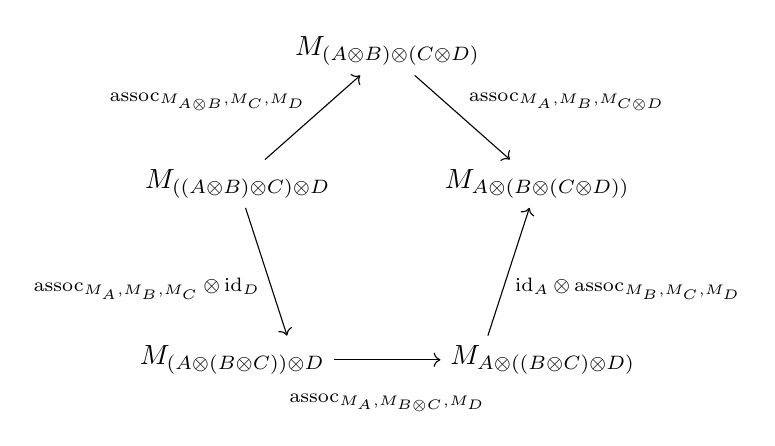
\begin{tikzpicture}[commutative diagrams/every diagram]
    \node (P0) at (90:2.3cm) {$M_{(A\tensor B)\tensor(C\tensor D)}$};
    \node (P1) at (90+72:2cm) {$M_{((A\tensor B)\tensor C)\tensor D}$} ;
    \node (P2) at (90+2*72:2cm) {\makebox[5ex][r]{$M_{(A\tensor(B\tensor C))\tensor D}$}};
    \node (P3) at (90+3*72:2cm) {\makebox[5ex][l]{$ M_{A\tensor((B\tensor C)\tensor D)} $}};
    \node (P4) at (90+4*72:2cm) {$ M_{A\tensor(B\tensor(C\tensor D))} $};
  \path[commutative diagrams/.cd, every arrow, every label]
    (P1) edge node {$\assoc_{M_{A\tensor B},M_C,M_D}$} (P0)
    (P1) edge node[swap] {$\assoc_{M_A,M_B,M_C}\tensor\id_D$} (P2)
    (P2) edge node[swap, yshift=-1em] {$\assoc_{M_A,M_{B\tensor C},M_D}$} (P3)
    (P3) edge node[swap] {$\id_A\tensor\assoc_{M_B,M_C,M_D}$} (P4)
    (P0) edge node {$\assoc_{M_A,M_B,M_{C\tensor D}}$} (P4);
  \end{tikzpicture}
  \]
which immediately gives rise to a second commutative diagram in $\Set$:
\[
  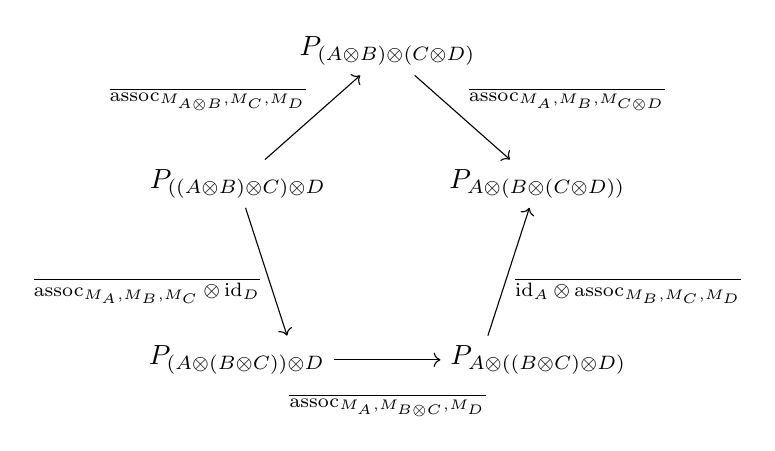
\begin{tikzpicture}[commutative diagrams/every diagram]
    \node (P0) at (90:2.3cm) {$P_{(A\tensor B)\tensor(C\tensor D)}$};
    \node (P1) at (90+72:2cm) {$P_{((A\tensor B)\tensor C)\tensor D}$} ;
    \node (P2) at (90+2*72:2cm) {\makebox[5ex][r]{$P_{(A\tensor(B\tensor C))\tensor D}$}};
    \node (P3) at (90+3*72:2cm) {\makebox[5ex][l]{$ P_{A\tensor((B\tensor C)\tensor D)} $}};
    \node (P4) at (90+4*72:2cm) {$ P_{A\tensor(B\tensor(C\tensor D))} $};
  \path[commutative diagrams/.cd, every arrow, every label]
    (P1) edge node {$\overline{\assoc_{M_{A\tensor B},M_C,M_D}}$} (P0)
    (P1) edge node[swap] {$\overline{\assoc_{M_A,M_B,M_C}\tensor\id_D}$} (P2)
    (P2) edge node[swap, yshift=-1em] {$\overline{\assoc_{M_A,M_{B\tensor C},M_D}}$} (P3)
    (P3) edge node[swap] {$\overline{\id_A\tensor\assoc_{M_B,M_C,M_D}}$} (P4)
    (P0) edge node {$\overline{\assoc_{M_A,M_B,M_{C\tensor D}}}$} (P4);
  \end{tikzpicture}
  \]
But this is the image under the functor $\H$ of the following diagram in $\G_{\cc}(\alpha)$:
\[
  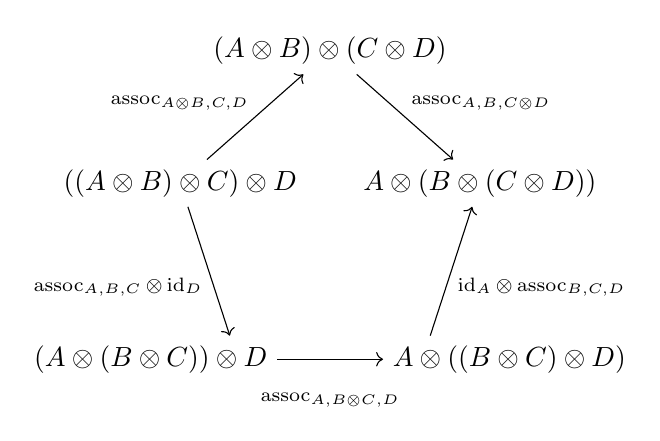
\begin{tikzpicture}[commutative diagrams/every diagram]
    \node (P0) at (90:2.3cm) {${(A\tensor B)\tensor(C\tensor D)}$};
    \node (P1) at (90+72:2cm) {${((A\tensor B)\tensor C)\tensor D}$} ;
    \node (P2) at (90+2*72:2cm) {\makebox[5ex][r]{${(A\tensor(B\tensor C))\tensor D}$}};
    \node (P3) at (90+3*72:2cm) {\makebox[5ex][l]{${A\tensor((B\tensor C)\tensor D)} $}};
    \node (P4) at (90+4*72:2cm) {${A\tensor(B\tensor(C\tensor D))} $};
  \path[commutative diagrams/.cd, every arrow, every label]
    (P1) edge node {$\assoc_{{A\tensor B},C,D}$} (P0)
    (P1) edge node[swap] {$\assoc_{A,B,C}\tensor\id_D$} (P2)
    (P2) edge node[swap, yshift=-1em] {$\assoc_{A,{B\tensor C},D}$} (P3)
    (P3) edge node[swap] {$\id_A\tensor\assoc_{B,C,D}$} (P4)
    (P0) edge node {$\assoc_{A,B,{C\tensor D}}$} (P4);
  \end{tikzpicture}
  \]
Since $\H$ is a faithful functor and the second diagram commutes, this last diagram must commute as well.  

It remains to show that $\assoc_{A,B,C},\lunit_A,\runit_A,\braid_{A,B}$ are natural transformations.  We show this for $\assoc_{A,B,C}$ and the other cases are entirely similar.  

Showing that $\assoc_{A,B,C}$ is a natural transformation from $((\blank\tensor \blank)\tensor \blank)$ to $(\blank\tensor(\blank\tensor \blank)\from \G(\alpha)\times\G(\alpha)\times\G(\alpha)\to\G(\alpha)$ means showing that the following diagram commutes for all completely negative $\alpha$-games $A',B',C',A,B,C$ and all morphisms $\sigma\from A'\to A,\tau\from B'\to B,\upsilon\from C'\to C$:
\[
  \begin{tikzcd}
    (A'\tensor B')\tensor C' \arrow[r, "(\sigma\tensor\tau)\tensor\upsilon"'] \arrow[d, "\assoc_{A', B', C'}"']
      & (A\tensor B)\tensor C \arrow[d, "\assoc_{A,B,C}"] \\
    A'\tensor(B'\tensor C') \arrow[r, "\sigma\tensor(\tau\tensor\upsilon)"']
      & A\tensor(B\tensor C)
  \end{tikzcd}
  \]
It is easy to check that this diagram commutes by applying the functor $\F\colon\G(\alpha)\to\Rel$.  The relational content $\grel{\assoc_{A,B,C}}$ of the strategy $\assoc_{A,B,C}$ is the graph of the function 
\[
  \overline{\assoc_{M_A,M_B,M_C}}\from P_{(A\tensor B)\tensor C}\to P_{A\tensor(B\tensor C)}
  \]
and its action by left composition on $\grel{(\sigma\tensor\tau)\tensor\upsilon}\subset P_{(A'\tensor B')\tensor C'}\times P_{(A\tensor B)\tensor C}$ is pointwise application of this function.  We find that
\begin{align*}
  \grel{\comp{\assoc_{A,B,C}}{(\sigma\tensor\tau)\tensor\upsilon}}
  &=\comp{\grel{\assoc_{A,B,C}}}{\grel{(\sigma\tensor\tau)\tensor\upsilon}}\\
  &=\left\{(s,t)\in P_{(A'\tensor B')\tensor C'}\times P_{A\tensor(B\tensor C)}\;\middle|\;\mbox{\pbox{\textwidth}{$(s\vert_{A'},t\vert_A)\in\grel{\sigma}$\\$(s\vert_{B'},t\vert_B)\in\grel\tau$\\$(s\vert_{C'},t\vert_C)\in\grel\upsilon$}}\right\}
\end{align*}
A similar argument now shows that $\grel{\comp{\sigma\tensor(\tau\tensor\upsilon)}{\assoc_{A', B', C'}}}$ is equal to the same set, and so we have a commutative diagram in $\Rel$:
\[
  \begin{tikzcd}
    P_{(A'\tensor B')\tensor C'} \arrow[r, "\grel{(\sigma\tensor\tau)\tensor\upsilon}"'] \arrow[d, "\grel{\assoc_{A', B', C'}}"']
      & P_{(A\tensor B)\tensor C} \arrow[d, "\grel{\assoc_{A,B,C}}"] \\
    P_{A'\tensor(B'\tensor C')} \arrow[r, "\grel{\sigma\tensor(\tau\tensor\upsilon)}"']
      & P_{A\tensor(B\tensor C)}
  \end{tikzcd}
  \]
Therefore, our original diagram in $\G(\alpha)$ is commutative, since the functor $\F$ is faithful.  

We therefore have the structure of a symmetric monoidal category on $\G(\alpha)$.  

\subsubsection{Symmetric monoidal closed structure}
\label{TransSMCCSex}

In existing finitary models of game semantics, the category of games is made into a symmetric monoidal closed category where the linear implication of two objects is given by the connective $\implies$.  As we remarked earlier, this approach will not work immediately for us, since $A\implies B$ need not be completely negative even if $A$ and $B$ are.  Our solution will be to modify $A\implies B$ so that it becomes completely negative.  

Remember that when we proved that the composition of strategies $\sigma\from A\implies B$ and $\tau\from B\implies C$ is well defined, we were careful not to require that $C$ be acn (or completely negative).  From the point of view of constructing a category whose objects are $\alpha$-games, this is not useful, but it does allow us to construct certain alternative categories.

\begin{definition}
  Recall that if $\C$ is a category and $A$ is an object of $\C$, then the \emph{slice category} $\C/A$ is the category where the objects are morphisms
  \[
    \map{f}{B}{A}
    \]
  where $B$ is an object of $\C$ and where the morphisms between an object $\map{f}{B}{A}$ and an object $\map{g}{C}{A}$ are commutative triangles:
  \[
    \begin{tikzcd}
      B \arrow[r, "f"] \arrow[d, "h"']
       & A \\
      C \arrow[ur, "g"]
        &
    \end{tikzcd}
    \]
  Let $A$ be a (not necessarily completely negative) $\alpha$-game.  Abusing notation slightly, we write $\G(\alpha)/A$ for the category whose objects are strategies
  \[
    \sigma\from B\implies A
    \]
  for $B$ a \emph{completely negative} $\alpha$-game and where the morphisms from an object $\map{\sigma}{B}{A}$ to an object $\map{\tau}{C}{A}$ are commutative triangles of the form
  \[
    \begin{tikzcd}
      B \arrow[r, "\sigma"] \arrow[d, "\upsilon"']
       & A \\
      C \arrow[ur, "\tau"]
        &
    \end{tikzcd}
    \]
\end{definition}

The main technical result we shall use to construct our closed monoidal structure is the following theorem:
\begin{theorem}
  \label{SliceTerminalObject}
  Let $A$ be an $\alpha$-game.  Then the category $\G(\alpha)/A$ has a terminal object.
\end{theorem}

Note that if $A$ is completely negative, then the terminal object of $\G(\alpha)/A$ is the identity strategy $\map{\id_A}{A}{A}$, as is standard for slice categories.  If $A$ is not completely negative, then we will need to use a different construction.

We will write this terminal object as $A^{\cn}\xrightarrow{\cn}A$.  $A^{\cn}$ should be thought of as the `smallest completely negative extension of $A$', and the fact that it gives rise to a terminal object in $\G(\alpha)/A$ makes this vague notion precise.  If $A$ and $B$ are completely negative $\alpha$-games, we shall define a game $A\impliescn B$ to be given by $(A\implies B)^{\cn}$.  We will then be able to use the fact that $(A\implies B)^{\cn}$ gives rise to a terminal object in the category $\G(\alpha)/(A\implies B)$ to show that the connective $\impliescn$ in fact gives rise to a monoidal closed structure on $\G(\alpha)$.  

\begin{definition}
  Let $A$ be an $\alpha$-game.  We form a completely negative $\alpha$-game $A^{\cn}$ as follows:
  \begin{itemize}
    \item $M_{A^{\cn}}=M_A\cprd \{*_t\suchthat \textrm{$t\in P_A$ is a limiting $O$-play}\}$
    \item $\lambda_{A^{\cn}}(x)=\lambda_A(x)$ for all $x\in M_A$.  $\lambda_{A^{\cn}}(*_s)=O$
    \item $\zeta_{A^{\cn}}(sx)=\lambda_{A^{\cn}}(x)$ for $sx\in P_{A^{\cn}}$ a successor play.
    \item $\zeta_{A^{\cn}}(s)=P$ for $s\in P_{A^{\cn}}$ a limiting play.
  \end{itemize}
  \[
    P_{A^{\cn}} = \left\{s\in \left(M_{A^{\cn}}\right)^{*<\alpha}\;\middle|\;\mbox{\pbox{200px}{
      $t\vert_{M_A}\in P_A$\\
      If $u*_t\prefix s$ then $u=t$. \\
      If $vx\prefix s$ and $v\vert_{M_A}$ is a limiting $O$-play in $P_A$ then $x=*_v$
    }}\right\}
    \]

  In other words, we force $A$ to be completely negative by making all limiting plays be $P$-plays.  If $u$ was a limiting $O$-play in $A$, then it becomes a $P$-play in $A^{\cn}$.  Since the moves that follow $u$ in $A$ are $P$-moves, we add in an extra $O$-move $*_u$ in order to preserve the alternating condition.
\end{definition}

\begin{example}
  If $\alpha=\omega$ and $A$ is a negative game then we have $\bneggame A^{\cn}\cong A\implies\bot$: the single move in $\bot$ takes the role of $*_{\emptyplay}$.  However, if $\alpha$ is a higher ordinal, then this does not hold, since $A\implies\bot$ is no longer a completely negative game.  

  If $A,B$ are completely negative $\alpha$-games, we define $A\impliescn B$ to stand for $(A\implies B)^{\cn}$.  Then we do have $\bneggame{A}^{\cn}\cong A\impliescn \bot$.  The object $A\impliescn B$ will be the linear implication in our category.
\end{example}

\begin{notation}
  Given a sequence $s\in P_{A^{\cn}}$, we may restrict $s$ to a play $s\vert_A\in P_A$ by removing all the $*$-moves.  
\end{notation}

Given an $\alpha$-game $A$, there is a natural strategy $\cn_A$ for $A^{\cn}\implies A$ given by
\[
  \cn_A = \left\{s\in P_{A^{\cn}\implies A}\suchthat\textrm{for all $P$-positions $t\prefix s$, $t\vert_{A^{\cn}}\vert_A=t\vert_A$}\right\}
  \]
Concretely, this strategy is the copycat strategy for $A$, with the difference that whenever we reach a limiting $O$-play $u$ in $A$, player $P$ plays the extra move $*_u$ in $A^{\cn}$ before continuing.

We claim that $\map{\cn_A}{A^{\cn}}{A}$ is the terminal object in the category $\G(\alpha)/A$.  To do that, it will suffice to prove the following proposition:

\begin{proposition}
  \label{CnUniversalProperty}
  $\cn_A$ is a total strategy for $A^{\cn}\implies A$.  Moreover, $\cn_A$ satisfies the following universal property: given a completely negative $\alpha$-game $B$ and a strategy $\sigma$ for $B\implies A$, there is a unique strategy $\sigma^{\cn}$ for $B\implies A^{\cn}$ such that the following diagram commutes:
  \[
    \begin{tikzcd}
      B \arrow[r, "\sigma^{\cn}"] \arrow[dr, "\sigma"']
        & A^{\cn} \arrow[d, "\cn_A"] \\
      %
        & A
    \end{tikzcd}
    \]
\end{proposition}

\begin{proof}
  We first show that $\cn_A$ is a valid strategy for $A^{\cn}\implies A$.  It is certainly prefix closed and satisfies the limiting condition by its definition.  Moreover, if $s\in\cn_A$ is a $P$-position and $sx\in P_{A^{\cn}\implies A}$ then $sx$ satisfies the conditions to be an element of $\cn_A$.

  Suppose that $sx, sy\in \cn_A$ are $P$-positions.  Suppose first that neither $x$ nor $y$ is a move of the form $*_t$.  We claim that $sx,sy$ take place in the same game.  Indeed, suppose instead that $x$ is a move in $A^{\cn}$ and $y$ is a move in $A$.  Then we have:
  \begin{gather*}
    s\vert_{A^{\cn}}\vert_A x = sx\vert_{A^{\cn}}\vert_A = sx\vert_A = s\vert_A\\
    s\vert_{A^{\cn}}\vert_A = sy\vert_{A^{\cn}}\vert_A = sy\vert_A = s\vert_Ay
  \end{gather*}
  which is a contradiction since it implies that $s\vert_{A^{\cn}}\vert_A$ is simultaneously a shorter sequence than $s\vert_A$ and a longer sequence than $s\vert_A$.

  If $x,y$ are both moves in $A^{\cn}$ then we have
  \begin{align*}
    s\vert_{A^{\cn}}\vert_A x &= sx\vert_{A^{\cn}}\vert_A \\
    & = sx\vert_A\\
    & = s\vert_A
  \end{align*}
  and $s\vert_{A^{\cn}}\vert_Ay=s\vert_A$ by an identical argument, and so $x=y$.  Similarly, if $x,y$ are both moves in $A$, then we have:
  \begin{align*}
    s\vert_A x &= sx\vert_A \\
    &= sx\vert_{A^{\cn}}\vert_A\\
    &= s\vert_{A^{\cn}}\vert_A
  \end{align*}
  and similarly for $y$, so $x=y$.

  Now, without loss of generality assume that $x=*_t$ for some $t$.  Then $s\vert_{A^{\cn}}\vert_A$ is a limiting play.  Suppose for a contradiction that $y$ is a move in $A$.  Then we have:
  \[
    s\vert_{A^{\cn}}\vert_A = sy\vert_{A^{\cn}}\vert_A=sy\vert_A = s\vert_Ay
    \]
  which is a contradiction, since $s\vert_Ay$ is a successor play.  Therefore, $y$ is a move in $A^{\cn}$.  We have:
  \begin{align*}
    t &= s\vert_{A^{\cn}}\vert_A\\
    &= s*_t\vert_{A^{\cn}}\vert_A\\
    &= s*_t\vert_{A^{\cn}}\vert_A\\
    &= s\vert_{A^{\cn}}\vert_A
  \end{align*}
  Therefore, $s\vert_{A^{\cn}}\vert_A$ is a limiting $O$-play in $A$ and therefore we have $x=y=*_t$ by the definition of $A^{\cn}$.  

  Now we show that $\cn_A$ is total.  Suppose that $s\in\cn_A$ is an $O$-position.  Then $s\vert_{A^{\cn}}$ is a $P$-position and $s\vert_A$ is an $O$-position.  Suppose that $s=ty$ is a successor play.  Note that $y$ cannot be a $*$-move, since these are all $O$-moves occurring in $A^{\cn}$.  If $y$ takes place in $A^{\cn}$ then we have $t\vert_{A^{\cn}}\vert_A=t\vert_A$ and therefore player $P$ can play $y$ in $A$ and still be playing according to $\cn$.  Similarly, if $y$ takes place in $A$, then player $P$ can play $y$ in $A^{\cn}$ and be in accordance with $\cn_A$.  

  Suppose instead that $s$ is a limiting play.  It is clear from the definition that $s\vert_{A^{\cn}}\vert_A$ and $s\vert_A$ are both cofinal in $s$, so they are both limiting plays.  Therefore, $s\vert_A$ is a limiting $O$-play in $A$ and $s\vert_{A^{\cn}}\vert_A$ must be the corresponding $P$-play in $A^{\cn}$.  Therefore, player $P$ may play $*_t$ (where $t=s\vert_A$) in $A^{\cn}$ and still be in accordance with $A^{\cn}$.  So $\cn_A$ is total.

  Let $q\in P_A$.  We claim that there is some $s\in\cn_A$ such that $s\vert_A=q$.  Indeed, since Player $P$ makes all $*$-moves in $A^{\cn}\implies A$, player $O$ has a strategy for $A^{\cn}\implies A$ in which he plays the moves of the sequence $q$ in order.  Since the strategy $\cn_A$ is total, player $P$ always has a reply to Player $O$'s moves and the resulting sequence $s$ satisfies $s\vert_A=q$.  

  Therefore, the relational presentation of $\cn_A$ has the following property: for all sequences $q\in P_A$, there exists some $r\in P_{A^{\cn}}$ such that $(r,q)\in\grel{\cn_A}$.  Moreover, it is not difficult to see that this $r$ is unique, since play passes from $A$ to $A^{\cn}$ without fail at each turn, so a $P$-position in $\cn_A$ is uniquely determined by its sequence of $O$-moves, which must agree with its $A$-component.  

  In other words, the relational presentation $\grel{\cn_A}$ is the graph of an injective function $h\colon P_A\to P_{A^{\cn}}$.

  Let $B$ be a completely negative $\alpha$-game and let $\sigma$ be a strategy for $B\implies A$.  We define the strategy $\sigma^{\cn}$ for $B\implies A^{\cn}$ as follows:
  \[
    \sigma^{\cn} = \{s\in P_{B\implies A^{\cn}}\suchthat s\vert_{B,M_A}\in\sigma\}
    \]
  where we write $s\vert_{B,M_A}$ for the sequence obtained by deleting all $*$-moves from $s$.  

  $\sigma^{\cn}$ is prefix closed, since $\sigma$ is, and satisfies the limit condition, since $\sigma$ does.  Suppose that $s\in\sigma^{\cn}$ is a $P$-position and that $sx\in P_{B\implies A^{\cn}}$.  If $x$ is a $*$-move, then we have $sx\vert_{B,M_A}=s\vert_{B,M_A}\in\sigma$, so $sx\in\sigma^{\cn}$.  Otherwise, we have $sx\vert_{B,M_A}=s\vert_{B,M_A}x$.  

  If $s\vert_{B,M_A}$ is a $P$-position in $B\implies A$ then $s\vert_{B,M_A}x\in\sigma$ and therefore $sx\in\sigma^{\cn}$.  So suppose instead that $s\vert_{B,M_A}$ is an $O$-position.  If $s=ty$ is a successor position then $y$ is a $P$-move in $B\implies A^{\cn}$, so in particular $y$ is not a $*$-move and therefore $s\vert_{B,M_A}=t\vert_{B,M_A}y$ is a $P$-position.  Therefore, $s$ must be a limiting play.  

  Since $s$ is a $P$-position, $s\vert_B$ must be a $P$-position, $s\vert_{A^{\cn}}\vert_A$ must be an $O$-position in $A$ and $s\vert_{A^{\cn}}$ must be a $P$-position in $A^{\cn}$.  It follows that $u\coloneqq s\vert_{A^{\cn}}\vert_A$ is a limiting $O$-play.  It follows that $x$ is a move in $A^{\cn}$, and therefore that $x=*_u$, which is a case we have already dealt with.

  Next, suppose that $sx, sy\in\sigma^{\cn}$ are $P$-positions.  In particular, $x,y$ are not $*$-moves and we have $s\vert_{B,M_A}x,s\vert_{B,M_A}y\in\sigma$.  Therefore, $x=y$.  So $\sigma^{\cn}$ is a strategy.

  Lastly, suppose that $\sigma$ is a total strategy.  Let $s\in\sigma^{\cn}$ be an $O$-position in $B\implies A^{\cn}$.  Then $s\vert_B$ is a $P$-position in $B$ and $s\vert_{A^{\cn}}$ is an $O$-position in $A^{\cn}$.  So $s\vert_{A^{\cn}}$ is a successor play in $A^{\cn}$, since $A^{\cn}$ is completely negative.  If the last move of $s\vert_{A^{\cn}}$ is not a $*$-move then $s\vert_{A^{\cn}}\vert_A$ has the same last move as $s\vert_{A^{\cn}}$ and is therefore an $O$-position as well.  Then $s\vert_{B,M_A}$ is an $O$-position and so there is some $x\in P_{B\implies A}$ such that $s\vert_{B,M_A}x\in\sigma$. Then $sx\in P_{B\implies A^{\cn}}$ and so $sx\in\sigma^{\cn}$.  

  Suppose instead that $s\vert_{A^{\cn}}=t*_u$, where $u=t\vert_A$.  Then $u$ is an $O$-position in $A$, so $s\vert_{B,M_A}$ is an $O$-position in $B\implies A$ and therefore there is some $x\in P_{B\implies A}$ such that $s\vert_{B,M_A}x\in\sigma$.  Then $sx\in\sigma^{\cn}$.  So $\sigma^{\cn}$ is a total strategy.

  We claim that $\comp{\grel{\cn_A}}{\grel{\sigma^{\cn}}}=\grel\sigma$.  Then we will have $\comp{\cn_A}{\sigma^{\cn}}=\sigma$ by Lemma \ref{TransHylandSchalkFaithful} and Corollary \ref{TransHylandSchalkIsFunctor}.  Suppose $(s,t)\in\comp{\grel{\cn_A}}{\grel{\sigma^{\cn}}}$.  Then there is some $u\in P_{A^{\cn}}$ such that $(s,u)\in\grel{\sigma^{\cn}}$ and $(u,t)\in\grel{\cn_A}$.  Therefore, $(s,u\vert_A)\in\grel\sigma$ and $t=u\vert_A$.  It follows that $(s,t)\in\grel{\sigma}$, so $\comp{\grel{\cn_A}}{\grel{\sigma^{\cn}}}\subset\grel\sigma$.  

  To show the reverse inclusion, we shall use the following lemma, which we shall prove later.  

  \begin{lemma}
    \label{CnLiftingLemma}
    Let $B$ be a completely negative $\alpha$-game, let $A$ be an arbitrary $\alpha$-game and let $\sigma$ be a strategy for $B\implies A$.  Let $s\in\sigma$ be a $P$-position.  Then there is a unique $P$-position $t\in B\implies A^{\cn}$ such that $t\vert_{B,M_A}=s$.
  \end{lemma}

  We use Lemma \ref{CnLiftingLemma} to show the reverse inclusion as follows: let $s\in\sigma$ be a $P$-position -- so $(s\vert_B,s\vert_A)$ is an arbitrary element of $\grel\sigma$.  By Lemma \ref{CnLiftingLemma} there exists $t\in B\implies A^{\cn}$ such that $t\vert_{B,M_A}=s$.  In particular, $t\vert_{A^{\cn}}\vert_A=s\vert_A$ and $t\vert_B=s\vert_B$.  So we have $(s\vert_B,t\vert_{A^{\cn}})\in\grel{\sigma^{\cn}}$ and $(t\vert_{A^{\cn}},s\vert_A)\in\grel{\cn_A}$.  It follows that $(s\vert_B,s\vert_A)\in\grel{\sigma}$.  So $\grel\sigma\subset\comp{\grel{\cn_A}}{\grel{\sigma^{\cn}}}$.  

  Lastly, we need to show that the strategy $\sigma^{\cn}$ is unique.  Suppose that there were some other strategy $\tau$ for $B\implies A^{\cn}$ making the diagram commute:
  \[
    \begin{tikzcd}
      B \arrow[r, "\tau"] \arrow[dr, "\sigma"']
        & A^{\cn} \arrow[d, "\cn_A"] \\
      %
        & A
    \end{tikzcd}
    \]
  We shall show that $\grel\tau=\grel{\sigma^{\cn}}$ -- so $\tau=\sigma^{\cn}$.  First suppose that $s\in\sigma^{\cn}$ is a $P$-position.  Since $\sigma = \comp{\cn_A}{\tau}$, there is some sequence $\s\in\tau\|\cn_A$ such that $\s\vert_{B,A}=s\vert_{B,M_A}$.  We have $\s\vert_{A^{\cn}}\vert_A=\s\vert_A$ and therefore $s\vert_{B,M_A}=\s\vert_{B,A^{\cn}}\vert_{B,M_A}$.  Therefore, $s=\s\vert_{B,A^{\cn}}\in\tau$, by uniqueness in Lemma \ref{CnLiftingLemma}.  So $\grel{\sigma^{\cn}}\subset\grel{\tau}$.  

  Conversely, suppose that $s\in\tau$ is a $P$-position.  Then our argument above tells us that we have $(s\vert_{A^{\cn}},s\vert_{A^{\cn}}\vert_A)\in\grel{\cn_A}$.  So $(s\vert_B,s\vert_{A^{\cn}}\vert_A)\in\grel\sigma$.  Therefore there is some $P$-position $u\in\sigma$ such that $u\vert_B=s\vert_B$ and $u\vert_A=s\vert_{A^{\cn}}\vert_A$.  By Lemma \ref{CnLiftingLemma}, there is a sequence $t\in\sigma^{\cn}$ with $t\vert_{B,M_A}=s$.  Then we have
  \[
    (s\vert_B,s\vert_{A^{\cn}})=(t\vert_B,t\vert_{A^{\cn}})\in\grel{\sigma^{\cn}}
    \]
  and therefore $\grel\tau\subset\grel{\sigma^{\cn}}$.  
\end{proof}

It remains to prove Lemma \ref{CnLiftingLemma}.  

\begin{proof}[Proof of Lemma \ref{CnLiftingLemma}]
  This proof is similar to the proof of \ref{TransLiftingLemma}.  We inductively construct a sequence $t^0\prefix t^1\prefix\dots\prefix t^\gamma\prefix\dots\prefix t^\beta$, where $t^\gamma$ has length $\gamma$ and $t^\beta$ is our desired sequence $t$.  We shall prove inductively that $t^\gamma$ is the unique element $u\in\sigma^{\cn}$ of length $\gamma$ such that $u\vert_{B,M_A}=t$.

  If $\gamma$ is a limit ordinal, then set $t^\gamma$ to be the limit of all the sequences $t^\delta$ for $\delta<\gamma$.  We have $r\vert_{B,M_A}\prefix s$ for all proper prefixes $r\pprefix t^{\gamma}$ and therefore $t^\gamma\vert_{B,M_A}\prefix s$.  For uniqueness, suppose that $u^\gamma$ has length $\gamma$ and $u^\gamma\vert_{B,M_A}\prefix s$.  If $\delta<\gamma$ and we write $u^\delta$ for the prefix of $u^\gamma$ of length $\delta$ then we have $u^\delta=t^\delta$ by uniqueness and it follows that $u^\gamma=t^\gamma$.

  Suppose instead that $\gamma=\delta+1$ is a successor ordinal.  We have a sequence $t^\delta$ of length $\delta$.  

  Suppose first that $t^\delta$ is an $O$-position.  Then, as usual, $t^\delta\vert_{B,M_A}$ is an $O$-position.  We have $t^\delta\vert_{B,M_A}\prefix s$; since $s$ is a $P$-position, this must be a proper prefix, so there is some move $x$ such that $t^\delta\vert_{B,M_A}x\prefix s$.  By the argument above (showing that $\sigma^{\cn}$ is total if $\sigma$ is total), we must have $t^\delta x\in\sigma$.  We set $t^{\delta+1}=t^\delta x$.  Then $t^{\delta+1}\vert_{B,M_A}\prefix s$.  

  For uniqueness, suppose that $u^{\delta+1}$ is some other sequence of length $\delta+1$ with $u^{\delta+1}\vert_{B,M_A}\prefix s$.  Writing $u^{\delta+1}=u^\delta y$, we have $u^{\delta}=t^\delta$ by uniqueness for sequences of length $\delta$.  Then $t^\delta x,t^\delta y\in\sigma$ and so $x=y$.  So $u^{\delta+1}=t^{\delta+1}$.  

  Now suppose that $t^\delta$ is a $P$-position.  We have $t^\delta\vert_{B,M_A}\prefix s$.  If $t^\delta\vert_{B,M_A}=s$ then we terminate, setting $\beta=\delta$.  Otherwise, there is some move $x$ such that $t^\delta\vert_{B,M_A}x\prefix s$.  

  Suppose that $t^\delta\vert_{B,M_A}$ is a $P$-position.  Then $x$ is an $O$-move, so $t^\delta x$ is alternating.  \textbf{Since $B$ is completely negative}, Proposition \ref{NiceAcnGames} tells us that $t^\delta x\in P_{B\implies A^{\cn}}$.  Therefore, $t^\delta x\in\sigma^{\cn}$, since $\sigma^{\cn}$ is a strategy.  We set $t^{\delta+1}=t^\delta x$.  Then we certainly have $t^{\delta+1}\vert_{B,M_A}\prefix s$.  For uniqueness, suppose that $u^{\delta+1}$ has length $\delta+1$ and that $u^{\delta+1}\vert_{B,M_A}\prefix s$.  Then $u^{\delta+1}=t^\delta y$ for some $y$ by uniqueness for sequences of length $\delta$.  Since $t^\delta\vert_{B,M_A}$ is a $P$-position, it is in particular not a limiting $O$-play, so $y$ cannot be a $*$-move.  Therefore, we have $u^{\delta}\vert_{B,M_A}y\prefix s$ and so $x=y$.  

  Suppose instead that $t^\delta\vert_{B,M_A}$ is an $O$-position.  Then $v\coloneqq t^\delta\vert_{A^{\cn}}\vert_A$ must be a limiting $O$-play.  We set $t^{\delta+1}=t^\delta *_v$.  Since $*_v$ is the only move possible in position $t^\delta$, this must certainly be unique, and we have $t^\delta *_v\vert_{B,M_A}=t^\delta\vert_{B,M_A}\prefix s$.  

  This completes the proof by induction.
\end{proof}

\subsubsection{A digression}
\label{DigressionSex}

Earlier on, we defined a category $\G(\alpha)/A$ for $A$ an arbitrary $\alpha$-game.  At this point, it is tempting to define a category as follows:

\begin{definition}
  The objects of the category $\tilde{\G}(\alpha)$ are (not necessarily completely negative) $\alpha$-games.  If $A,B$ are $\alpha$-games, a morphism in $\tilde{\G}(\alpha)$ from $A$ to $B$ is a functor
  \[
    \F\from\G(\alpha)/A\to\G(\alpha)/B
    \]
  that commutes with the natural projection functors $p_A\from\G(\alpha)/A\to\G(\alpha)$ and $p_B\from\G(\alpha)/B\to\G(\alpha)$.  
\end{definition}

This definition is useful because we have a natural embedding (the $2$-Yoneda embedding) of $\G(\alpha)$ into the category $\tilde{\G}(\alpha)$ that sends a completely negative game $N$ to the category $\G/N$ and sends a morphism $\sigma\from M\implies N$ to the `post-composition with $\sigma$' functor between the slice categories $\G(\alpha)//M$ and $\G(\alpha)/N$.  

It is well known that this is a fully faithful embedding.  I claim that it is also essentially surjective, so it is in fact an equivalence of categories.  Indeed, this follows from what we have just shown:

\begin{proposition}
  Let $A$ be an arbitrary $\alpha$ game.  Then the categories $\G(\alpha)/A$ and $\G(\alpha)/A^{\cn}$ are isomorphic as categories, via an isomorphism that commutes with the projection functors.

  \begin{proof}
    We have a natural functor from $\G(\alpha)/A^{\cn}$ to $\G(\alpha)/A$ given by post-composition with $\cn_A$, where functoriality follows from associativity of composition.  This functor certainly commutes with the projection functors.  Then Proposition \ref{CnUniversalProperty} tells us that it is fully faithful and a bijection on objects, so it is a categorical isomorphism.
  \end{proof}
\end{proposition}

Therefore, the categories $\G(\alpha)$ and $\tilde{\G}(\alpha)$ are equivalent.  This suggests one strategy for defining a symmetric monoidal closed structure on $\G(\alpha)$: since the objects of $\tilde{\G}(\alpha)$ are not required to be completely negative, we may freely define a closed monoidal structure on $\tilde{\G}(\alpha)$ by setting the linear implication between games $A$ and $B$ to be the game $A\implies B$ and the tensor product to be the game $A\tensor B$.  This symmetric monoidal closed structure will give rise to a symmetric monoidal closed structure on $\G(\alpha)$ via the equivalence of categories.  

However, there is still quite a lot of work to show that this does indeed give a symmetric monoidal closed structure on $\tilde{\G}(\alpha)$, and it will be easier to construct the closed structure on $\G(\alpha)$ directly.

\subsubsection{The completely negative linear implication $A\impliescn B$}
\label{ImpliesCnSex}

Let $A,B$ be completely negative $\alpha$-games.  We have a completely negative $\alpha$-game $A\impliescn B\coloneqq (A\implies B)^{\cn}$.  We shall construct a monoidal closed structure on $\G(\alpha)$ where the linear implication between $A$ and $B$ is $A\impliescn B$.  

We shall start off with the relevant result about the (usual) implication $A\implies B$:

\begin{proposition}
  \label{impliesTreeIsom}
  Let $A,B,C$ be completely negative $\alpha$ games.  Then the games $(A\tensor B)\implies C$ and $A\implies(B\implies C)$ are tree isomorphic.
\end{proposition}

\begin{note}
  Since $(A\tensor B)\implies C$ is not a completely negative game in general, we cannot say that these games are isomorphic as objects of $\G(\alpha)$, but it will help us to know that they are tree-isomorphic as games.
\end{note}

\begin{proof}[Proof of Proposition \ref{impliesTreeIsom}]
  The sets of plays $P_{(A\tensor B)\implies C}$ and $P_{A\implies(B\implies C)}$ are both appropriate subsets of $P_A\|P_B\|P_C$.  We just need to check that $\lambda_{(A\tensor B)\implies C}=\lambda_{A\implies(B\implies C)}$ and that $\zeta_{(A\tensor B)\implies C}=\zeta_{A\implies(B\implies C)}$.  

  We have
  \begin{align*}
    \lambda_{(A\tensor B)\implies C} &= \neg\circ\lambda_{A\tensor B}\cprd\lambda_C\\
    &= \neg\circ\lambda_A\cprd\neg\circ\lambda_B\cprd\lambda_C\\
    &= \neg\circ\lambda_A\cprd\lambda_{B\implies C}\\
    &= \lambda_{A\implies(B\implies C)}
  \end{align*}
  and
  \begin{align*}
    \zeta_{(A\tensor B)\implies C}(s) & = ((\zeta_A(s\vert_A)\wedge\zeta_B(s\vert_B))\Rightarrow\zeta_C(s\vert_C))\\
    &=(\zeta_A(s\vert_A)\Rightarrow(\zeta_B(s\vert_B)\Rightarrow\zeta_C(s\vert_C))) \\
    &=\zeta_{A\implies(B\implies C)}(s)
  \end{align*}
  where we can prove the second equality as follows: if $p,q,r\in\OP$, then $((p\wedge q)\Rightarrow r) = O$ if and only if $p=q=P$ and $r=O$.  Meanwhile, $(p\Rightarrow (q\Rightarrow r))=O$ if and only if $p=q=P$ and $r=O$.  So $((p\wedge q)\Rightarrow r) = (p\Rightarrow(q\Rightarrow r))$.
\end{proof}

To construct the monoidal closed structure, it suffices to give a morphism
\[
  \ev_{A,B}\from (A\impliescn B)\tensor A\to B
  \]
for all pairs $(A,B)$ of completely negative $\alpha$-games, such that for all completely negative $\alpha$-games $X$ and all morphisms $\sigma\from X\tensor A\to B$ there is a unique morphism $\upsilon\from X\to A\impliescn B$ making the following diagram commute:
\[
  \begin{tikzcd}
    X\tensor A_3 \arrow[r, "\sigma"] \arrow[d, "\upsilon\tensor\id_A"']
      & B_2 \\
    (A_1\impliescn B_1)\tensor A_2 \arrow[ur, "\ev_{A,B}"']
      &
  \end{tikzcd}
  \]
(Here we have numbered the copies of $A$ and $B$ so we can refer to them individually).

The strategy $\ev_{A,B}$ for $((A\impliescn B)\tensor A)\implies B$ is constructed as follows: we have our strategy $\cn_{A\implies B}$ for $(A\impliescn B)\implies(A\implies B)$.  By Proposition \ref{impliesTreeIsom}, this game is tree isomorphic to the game $((A\impliescn B)\tensor A)\implies B$, so we get the strategy $\ev_{A,B}$ by applying this tree isomorphism to the strategy $\cn_{A\implies B}$.  

We need to show that the strategy $\ev_{A,B}$ satisfies the property given above.  Let $X$ be a completely negative $\alpha$-game and let $\sigma$ be a strategy for $(X\tensor A)\implies B$.  Then $\sigma$ gives rise, via the tree isomorphism above, to a strategy $\tilde{\sigma}$ for $X\implies(A\implies B)$.  Since the tree isomorphism does nothing more than identify $P_{(X\tensor A)\implies B}$ with $P_{X\implies(A\implies B)}$ as subsets of $(M_X\cprd M_B\cprd M_C)^{*<\alpha}$, we may identify $\sigma$ and $\tilde{\sigma}$ as subsets of $(M_X\cprd M_A\cprd M_B)$.  

Similarly, we may identify $\ev_{A,B}$ with $\cn_{A\implies B}$ as subsets of 
\[
  \left(M_{A_1}\cprd M_{B_1}\cprd M_{A_2}\cprd M_{B_2}\right)^{*<\alpha}
  \]
where we have again labelled the different copies of $A$ and $B$ to avoid confusion.

The strategy $\tilde{\sigma}$ gives rise to a strategy ${\tilde{\sigma}}^{\cn}$ for $X\implies(A\impliescn B)$.  We claim that this ${\tilde{\sigma}}^{\cn}$ satisfies the property above.  

First, we show that $\comp{\ev_{A,B}}{({\tilde{\sigma}}^{\cn}\tensor\id_A)}=\sigma$.  By the definition of ${\tilde{\sigma}}^{\cn}$, we know that it makes the following diagram commute:
\[
  \begin{tikzcd}
    X \arrow[r, "{\tilde{\sigma}}^{\cn}"] \arrow[dr, "\tilde\sigma"']
      & A_1\impliescn B_1 \arrow[d, "\cn_{A\implies B}"] \\
    %
      & A_2\implies B_2
  \end{tikzcd}
  \]
where we have labelled the copies of $A$ and $B$ so we can tell them apart.  Therefore, we have
\[
  \tilde\sigma = \{\s\vert_{X,A_2,B_2}\suchthat \s\in{\tilde\sigma}^{\cn}\|\cn_{A\implies B}\}
  \]
where
\[
  {\tilde\sigma}^{\cn}\|\cn_{A\implies B} = \left\{\s\in \left(M_X\cprd M_{A_1}\cprd M_{B_1}\cprd M_{A_2}\cprd M_{B_2}\right)^{*<\alpha}\;\middle|\;\mbox{\pbox{\textwidth}{
    $\s\vert_{X,A_1,B_1}\in{\tilde\sigma}^{\cn}$\\
    $\s\vert_{A_1,B_1,A_2,B_2}\in\cn_{A\implies B}$
  }}\right\}
  \]
Now we have
\[
  \comp{\ev_{A,B}}{({\tilde\sigma}^{\cn}\tensor\id_A)}=
  \left\{\t\vert_{X,A_2,B_2}\suchthat\t\in\left({\tilde\sigma}^{\cn}\tensor\id_A\right)\|\ev_{A,B}\right\}
  \]
where
\[
  \left({\tilde\sigma}^{\cn}\tensor\id_A\right)\|\ev_{A,B}
  =\left\{\t\in\left(M_X\cprd M_{A_3}\cprd M_{A_1}\cprd M_{B_1}\cprd M_{A_2}\cprd M_{B_2}\right)^{*<\alpha}\;\middle|\;
  \mbox{\pbox{\textwidth}{
    $\t\vert_{X,A_1,B_1}\in{\tilde\sigma}^{\cn}$\\
    $\t\vert_{A_3,A_2}\in\id_A$\\
    $\t\vert_{A_2,B_2}\in\ev_{A,B}$
  }}\right\}
  \]
Remembering that we may identify $\ev_{A,B}$ with $\cn_{A\implies B}$ as sets of plays, we see that
\[
  \comp{\ev_{A,B}}{({\tilde\sigma}^{\cn}\tensor\id_A)}\subset\tilde\sigma=\sigma
  \]
since if $\t\in\left({\tilde\sigma}^{\cn}\tensor\id_A\right)\|\ev_{A,B}$ then we have $\t\vert_{X,A_1,B_1,A_2,B_2}\in{\tilde\sigma}^{\cn}\|\cn_{A\implies B}$ and so $\t\vert_{X,A_2,B_2}\in\tilde\sigma$.  

Conversely, let $s\in\tilde\sigma$ and write $s=\s\vert_{X,A_2,B_2}$, where $\s\in{\tilde\sigma}^{\cn}\|\cn_{A\implies B}$.  We may construct a sequence $\t\in\left({\tilde\sigma}^{\cn}\tensor\id_A\right)\|\ev_{A,B}$ with $\t\vert_{X,A_1,B_1,A_2,B_2}=\s$ by inserting before each $P$-move in $A_2$ the corresponding move in $A_3$ and inserting \emph{after} each $O$-move in $A_2$ the corresponding move in $A_3$.  Therefore:
\[
  \sigma\subset\comp{\ev_{A,B}}{({\tilde\sigma}^{\cn}\tensor\id_A)}
  \]
For uniqueness, suppose that we have a strategy $\upsilon$ for $X\implies(A\impliescn B)$ making the following diagram commute:
\[
  \begin{tikzcd}
    X\tensor A_3 \arrow[r, "\sigma"] \arrow[d, "\upsilon\tensor\id_A"']
      & B_2 \\
    (A_1\impliescn B_1)\tensor A_2 \arrow[ur, "\ev_{A,B}"']
      &
  \end{tikzcd}
  \]
Exactly the same argument then tells us that
\[
  \comp{\cn_{A\implies B}}{\upsilon}=\comp{\ev_{A,B}}{\upsilon\tensor\id_A}=\sigma=\tilde\sigma
  \]
(as sets of plays) and so $\upsilon={\tilde\sigma}^{\cn}$ by the uniqueness part of Proposition \ref{CnUniversalProperty}.

Therefore $\G(\alpha)$ has the structure of a symmetric monoidal category with tensor product given by $\tensor$ and linear implication given by $\impliescn$.  

\subsubsection{Win-games and winning strategies}

We shall not develop the theory of transfinite win-games in this report, leaving this work for future research.  The basic idea is as follows.  Let $\alpha$ be an ordinal of the form $\omega^\beta$.  We form a category $\G(\alpha+1)$ of games where the objects are acn $\alpha+1$-games.  

Given an acn $\alpha+1$-game $A$, we have an associated $\alpha$-game $A^\circ$ given by forgetting about the plays of length $\alpha$.  We call a total strategy $\sigma$ for $A^\circ$ \emph{winning} if every play of length $\alpha$ that is the limit of plays from $\sigma$ is a $P$-play in $A$.  

We can then show that winning strategies compose to give winning strategies, just as in the $\omega+1$-case.  The morphisms between objects $A$ and $B$ in our category will be winning strategies for $A^\circ\implies B^\circ$.  We can then show that this category inherits a closed monoidal structure from $\G(\alpha)$.  

This construction agrees with the previous one in the sense that $\G(\omega+1)$ and our original category $\mathcal W$ of win-games are isomorphic as categories.  

\section{Exponentials}

We want to model the exponential connective $\oc$ from linear logic in our game semantics.  We adapt the approach taken in \cite{laird02} and \cite{martinsthesis} to our transfinite games.

\begin{definition}
  Let $\G(\alpha)$ be a category of transfinite games and let $A$ be an object of $\G(\alpha)$.  Then the \emph{exponential} $\oc A$ is given as follows:
  \begin{itemize}
    \item $M_{\oc A} = A\times\omega$
    \item $\lambda_{\oc A} = \lambda_A\circ\pr_1$
  \end{itemize}

  Given an ordinal-indexed sequence $s$ taking values in $M_{\oc A}$ and some $n\in\omega$, we write $s\vert_n$ for the subsequence of $s$ consisting of terms of the form $(a,n)$.  Then define
  \[
    \oc P_A = \{s\in M_{\oc A}^{*<\alpha}\suchthat s\vert_n\in P_A\textrm{ for all }n\in \omega\}
    \]
  We define $\zeta_{\oc A}\from \oc P_A\to \OP$ by
  \[
    \zeta_{\oc A}(s) = \bigwedge_{n\in \omega} \zeta_A(s\vert_n)
    \]
  (Here, if $(b_n)\in\OP^\omega$ then we have $\bigwedge_{n\in\omega} b_n = P$ if $b_n=P$ for all $n$ and $\bigwedge_{n\in\omega}=O$ otherwise.)

  We define $P_{\oc A}$ to be the set of all sequences $s\in\oc P_A$ that are well formed with respect to $\zeta_{\oc A},\lambda_{\oc A}$ and are alternating with respect to $\zeta_{\oc A}$ and that satisfy the following property:
  
  \begin{itemize}
    \item If the term $(a,n)$ occurs in $s$, and if $m<n$, then there is some term $(b,m)$ that occurs earlier in the sequence $s$ than $(a,n)$.  
  \end{itemize}

  Then $\oc A=(M_{\oc A},\lambda_{\oc A},\zeta_{\oc A},P_{\oc A})$.  
\end{definition}

So $\oc A$ is like an infinite tensor product of copies of $A$ with the restriction that the first move must take place in the first copy and that moves may not take place in a subsequent copy of $A$ until moves have been made in all earlier copies.  

\begin{proposition}
  $\oc A$ is a well formed game.
  \begin{proof}
    Exactly the same argument from Proposition \ref{TransTensorWellFormed}.
  \end{proof}
\end{proposition}

Just like the tensor product, the exponential $\oc A$ has the property that only player $O$ may switch games:

\begin{proposition}
  \label{ExponentialWhoSwitchesGames}
  Suppose that $s(a,m)(b,n)\in P_{\oc A}$, where $m\ne n$.  Then $\lambda_{\oc A}(b,n)=O$.  
  \begin{proof}
    $\begin{aligned}[t]
      \lambda_{\oc A}(b,n) &= \zeta_{\oc A}(s(a,m)(b,n))\\
      &= \bigwedge_{k\in\omega}\zeta_A(s(a,m)(b,n)\vert_k)
    \end{aligned}$

    Now by alternation we must have either $\zeta_A(s\vert_m(a,m))=O$ or $\zeta_A(s\vert_n(b,n))=O$.  So this last expression must be equal to $O$.
  \end{proof}
\end{proposition}

We can also prove a version of Proposition \ref{NiceAcnGames} for the exponential connective using the same argument.

To demonstrate why it is important to restrict the order in which the opponent $O$ may open games, we define a commutative comonoid structure on $\oc A$.  The comultiplication $\mu\from \oc A\to \oc A\tensor \oc A$ is the copycat strategy that opens a new copy of $A$ on the left hand side whenever a new copy of $A$ is opened on the right hand side.  (Here we see why the condition on the order in which games may be opened is important -- if we had no such restriction then there would be no canonical way to choose which copy of $A$ to open on the left hand side and the comultiplication would not be associative.)

The counit $\eta\from \oc A\to I$ is the unique empty strategy on $\oc A\implies I$.  

For associativity of comultiplication, we want to check that the following diagram commutes:
\[
  \begin{tikzcd}
    \oc A \arrow[r, "\mu"] \arrow[dd, "\mu"']
      & \oc A \tensor \oc A \arrow[d, "\id_{\oc A}\tensor \mu"] \\
    %
      & \oc A \tensor (\oc A \tensor \oc A) \arrow[d, "\assoc_{A,A,A}\inv"] \\
    \oc A \tensor \oc A \arrow[r, "\mu\tensor\id_{\oc A}"']
      & (\oc A \tensor \oc A) \tensor \oc A
  \end{tikzcd}
  \]
For this, note that each path round the diagram is a copycat strategy $\oc A \to (\oc A\tensor \oc A)\tensor \oc A$.  Since we are forced to open copies of $\oc A$ in order, there is only one such copycat strategy, and so the two paths must be equal.  

Exactly the same argument tells us that comultiplication is commutative and that the counit is indeed a counit for this comultiplication.

We have a natural forgetful functor from the category of comonoids over $\G(\alpha)$ to $\G(\alpha)$ itself.  We first want to show that we have a functor in the opposite direction that sends a game $A$ to this comonoid over $\oc A$.  

Let $A,B$ be completely negative $\alpha$-games and let $\sigma$ be a strategy for $A\implies B$.  Then we have a natural strategy $\oc \sigma$ for $\oc A\implies\oc B$ given by
\[
  \oc\sigma = \{s\in P_{\oc A}\suchthat s\vert_n\in\sigma\textrm{ for all $n\in\omega$}\}
  \]
where we have written $s\vert_n$ for the subsequence of $s$ consisting of all terms that occur in the $n$-th copy of $A$ or the $n$-th copy of $B$.  

The proof that this is a strategy may be adapted from the discussion of the strategy $\sigma\tensor\tau$ above.  Similarly, we may show that if $A,B,C$ are completely negative $\alpha$-games and we have strategies $A\xrightarrow{\sigma}B\xrightarrow{\tau}C$ then
\[
  \comp{\oc\tau}{\oc\sigma} = \oc(\comp\tau\sigma)
  \]
using the same argument we used to show that taking the tensor product of two strategies preserves composition.

This gives us a functor $\cmap{\oc}{\G(\alpha)}{\G(\alpha)}$.  We want to show that it gives rise to a functor from $\G(\alpha)$ into the category of comonoids over $\G(\alpha)$ sending a game $A$ to the comonoid $\oc A\to \oc A\tensor \oc A$.  For this, we need to show that if $A,B$ are completely negative $\alpha$-games and $\sigma$ is a strategy for $A\implies B$ then the following diagram commutes:
\[
  \begin{tikzcd}
    \oc A \arrow[r, "\mu"] \arrow[d, "\oc \sigma"']
      & \oc A \tensor \oc A \arrow[d, "\oc \sigma \tensor \oc \sigma"] \\
    \oc B \arrow[r, "\mu"']
      & \oc B \tensor \oc B
  \end{tikzcd}
  \]
Each branch of this diagram is a strategy for $\oc A\implies(\oc B\tensor\oc B)$ in which player $P$ plays according to $\sigma$, opening a new copy of $A$ on the left each time player $O$ opens a copy of $B$ on the right.  Since the order in which player $P$ may open copies of $A$ is pre-determined, there is a unique such strategy, and so this diagram must commute.  

We shall eventually show that in fact $\oc A\to\oc A\tensor\oc A$ is the \emph{cofree commutative comonoid} on $A$.  To show that, we will need \cite{martinsthesis} to give a map $\der\from\oc A\to A$, and we will need to show that for each commutative comonoid $B\to B\tensor B$ and each morphism $\sigma\from B\to A$ there exists a unique morphism $\sigma^\dagger\from B\to \oc A$ such that the following diagram commutes:
\[
  \begin{tikzcd}
    A
      & \oc A \arrow[l, "\der"'] \arrow[r, "\mu"]
        & \oc A \tensor \oc A \\
    %
      & B \arrow[r] \arrow[u, dotted, "\sigma^\dagger"'] \arrow[ul, "\sigma"]
        & B\tensor B \arrow[u, dotted, "\sigma^\dagger \tensor \sigma^\dagger"']
  \end{tikzcd}
  \]
We are not yet in a position to define the morphism $\sigma^\dagger$, but it is easy to see what $\der$ is: it is the copycat strategy on $\oc A\implies\oc A$ that copies the moves from $A$ on the right into the first copy of $A$ on the left.  

\subsection{Products in $\G(\alpha)$}

Let $(A_i\suchthat i\in I)$ be a collection of objects of $\G(\alpha)$.  We define the product
\[
  \prod_i A_i
  \]
to be the game given by
\begin{itemize}
  \item $M_{\prod_i A_i}=\bigcprd_i M_{A_i}$
  \item $\lambda_{\prod_i A_i}=\bigcprd_i \lambda_{A_i}$
  \item $P_{\prod_i A_i} = \bigcprd_i P_{A_i}$
  \item $\zeta_{\prod_i A_i} = \bigcprd_i \zeta_{A_i}$
\end{itemize}
This is the game where Player $O$ may decide which of the $A_i$ to play his first move in; play then continues in that game and the other games are never used.  

We claim that $\prod_i A_i$ is the categorical product of the $A_i$ in $\G(\alpha)$.  First note that we have natural projection strategies $\pr_j$ for $\prod_i A_i\to A_j$ for each $j\in I$, in which player $P$ plays copycat in game $A_j$ on the left.  Now if $B$ is an object of $\G(\alpha)$ and $\sigma_i$ are strategies for $B\implies A_i$ for each $i\in I$, then we have a strategy $\sigma$ for $B\implies\prod_i A_i$ in which player $P$ uses strategy $j$ when player $O$'s initial move takes place in $A_j$:
\[
  \sigma = \bigcprd_i \sigma_i
  \]

We can see that $\comp{\pr_j}{\sigma}=\sigma_j$ for each $j$: indeed, $\grel{\pr_j}$ is the graph of the inclusion $P_{A_j}\hookrightarrow P_{\prod_i A_i}$, while $\grel\sigma$ is the union of the relations $\grel{\sigma_i}$, so this equation holds in the relational presentation:
\[
  \comp{\grel{\pr_j}}{\grel{\sigma}}=\grel{\sigma_j}
  \]
Moreover, it is easy to see that $\grel\sigma$ is the unique relation between $P_B$ and $P_{\prod_i A_i}$ such that this equation holds for all $j$, and therefore $sigma$ is the unique strategy for $B\implies\prod_i A_i$ such that $\comp{\pr_j}{\sigma}=\sigma_j$ for each $j\in I$.  Therefore, $\G(\alpha)$ has all small products.  

Given games $A,B$, we shall write $A\times B$ for the product of $A$ and $B$.

\subsection{The exponential as a final coalgebra}

Our definition of the exponential connective $\oc$ was different from the definitions of the other connectives in that it involved an explicit restriction on the order in which new games could be opened.  We saw that this restriction was necessary in order to guarantee associativity of the comultiplication in our comonoid, but it means that it is hard to study the exponential $\oc A$ using the connectives $\tensor$ and $\implies$.  

Let $A,B$ be objects of some category $\G(\alpha)$ of transfinite games.  Following \cite{laird02}, we define the \emph{sequoid} $A\sequoid B$ by:

\begin{itemize}
  \item $M_{A\sequoid B} = M_{A\tensor B}$
  \item $\lambda_{A\sequoid B}=\lambda_{A\tensor B}$
  \item $P_{A\sequoid B} = \{s\in P_{A\tensor B}\suchthat\textrm{$s=\emptyplay$ or the first move of $s$ takes place in $A$}\}$
  \item $\zeta_{A\sequoid B} = \zeta_{A\tensor B}\vert_{P_{A\sequoid B}}$
\end{itemize}

It is clear that $A\sequoid B$ is a well-formed game - namely, it is the weakening of the tensor product $A\tensor A$ such that player $O$ is forced to start play in the game $A$.  We have a natural copycat strategy $\wk\from A\tensor B\to A\sequoid B$ and the morphism
\[
  \dec_{A,B}\from A\tensor B\to (A\sequoid B)\times(B\sequoid A)
  \]
induced by the morphisms
\[
  A\tensor B\xrightarrow{\wk}A\sequoid B\quad A\tensor B\xrightarrow{\braid}B\tensor A\xrightarrow{\wk}B\sequoid A
  \]
is an isomorphism.

Other natural copycat isomorphisms may be verified by inspection:
\begin{gather*}
  \passoc_{A,B,C} \from (A\sequoid B) \sequoid C \toisom A\sequoid (B\tensor C) \\
  \pcomm_{A,B,C} = \comp{\passoc_{A,B,C}\inv}{\comp{(\id_A\tensor\braid)}{\passoc_{A,B,C}}} \from (A\sequoid B)\sequoid C \toisom (A\sequoid C)\sequoid B\\
  \lun_A \from I\sequoid A \toisom I\\
  \run_A \from A\sequoid I \toisom A \\
  \dist_{A,B,C}=\langle \pi_1\sequoid\id_C,\pi_2\sequoid\id_C\rangle\from (A\times B)\sequoid C \toisom (A\sequoid C)\times(B\sequoid C)
\end{gather*}

One important point is that the sequoid does not give rise to a functor $\G(\alpha)\times\G(\alpha)\to\G(\alpha)$ in the way that the tensor product does.  To see why, let $A,B,C,D$ be games, let $\sigma$ be a strategy for $A\implies B$ and let $\tau$ be a strategy for $C\implies D$.  We would like to construct a strategy $\sigma\sequoid\tau$ for
\[
  (A\sequoid C)\implies (B\sequoid D)
  \]
in which player $P$ plays according to $\sigma$ in $A$ and $B$ and according to $\tau$ in $B$ and $D$, exactly as in the strategy $\sigma\tensor\tau$.  The problem is that $\sigma\tensor\tau$ is not necessarily a valid strategy for $(A\sequoid C)\implies (B\sequoid D)$, even if $\sigma$ is a valid strategy for $A\implies B$ and $\tau$ is a valid strategy for $C\implies D$.  

Indeed, suppose that player $P$'s reply in $\sigma$ to a particular opening move in $B$ is also a move in $B$, and suppose further that player $P$'s reply in $\tau$ to a particular opening move in $D$ is a move in $C$ (for example, if $\tau$ is a copycat strategy).  Now consider the following narrative for the game $(A\sequoid C)\implies (B\sequoid D)$:
\begin{enumerate}
  \item Player $O$ plays the opening move in $B$, as he must.
  \item Player $P$ replies in $B$, according to $\sigma$.  
  \item Player $O$ decides to switch and start the game $D$.
  \item According to $\tau$, player $P$ should reply with a move in $C$.  But she cannot play in $C$, since no moves have been played in $A$ yet.
\end{enumerate}

In order to fix this situation, we place a restriction on the strategy $\sigma$.

\begin{definition}
  Let $A,B$ be objects of $\G(\alpha)$.  A strategy $\sigma$ for $A\implies B$ is called \emph{strict} if player $P$'s reply to each opening $O$-move in $B$ is a move in $A$ - so if $bx\in\sigma$ then $x\in M_A$.

  It is easy to see that the composition of strict strategies $\sigma$ for $A\implies B$ and $\tau$ for $B\implies C$ is a strict strategy for $A\implies C$ and that the identity strategy is strict.  Therefore, we have a full-on-objects subcategory $\G_s(\alpha)$ of $\G(\alpha)$ of games and strict strategies.
\end{definition}

\begin{proposition}
  Let $A,B,C,D$ be objects of $\G(\alpha)$, let $\sigma$ be a strict strategy for $A\implies B$ and let $\tau$ be a strict strategy for $C\implies D$.  Then $\sigma\sequoid\tau=\sigma\tensor\tau\cap P_{(A\sequoid C)\implies (B\sequoid D)}$ is a strict strategy for $(A\sequoid C)\implies (B\sequoid D)$ and the following diagram commutes (so $\wk$ is a natural transformation between $\blank\tensor\blank$ and $\blank\sequoid\blank$):
  \[
    \begin{tikzcd}
      A\tensor C \arrow[r, "\sigma\tensor\tau"] \arrow[d, "\wk"']
        & B\tensor D \arrow[d, "\wk"] \\
      A\sequoid C \arrow[r, "\sigma\sequoid\tau"']
        & B\sequoid D
    \end{tikzcd}
    \]

  \begin{proof}
    We know that $\sigma\tensor\tau$ is a valid strategy for $(A\tensor C)\implies (B\tensor D)$, so we just need to check that no moves in $B$ take place before moves in $D$ and that no moves in $A$ take place before moves in $C$.  Indeed, player $O$'s opening move must take place in $B$; then, since $\sigma$ is strict, player $P$'s reply will take place in $A$.  So $\sigma\sequoid\tau$ is a valid strategy for $(A\sequoid C)\implies(B\sequoid D)$; moreover, it is itself a strict strategy.
  \end{proof}
\end{proposition}

What this means is that $\blank\sequoid\blank$ gives us a functor, not from $\G(\alpha)\times\G(\alpha)$ to $\G(\alpha)$, but from $\G_s(\alpha)\times\G(\alpha)$ to $\G_s(\alpha)$.  In fact, the isomorphism $\passoc\from (A\sequoid B)\sequoid C\cong A\sequoid(B\tensor C)$ tells us that $\blank\sequoid\blank$ is a \emph{right action} of the monoidal category $\G(\alpha)$ upon the category $\G_s(\alpha)$.  

The closed monoidal category $\G(\alpha)$, the subcategory $\G_s(\alpha)$, the morphisms $\passoc$ and $\run$, and the natural transformation $\wk$ in fact give rise to a structure known as a \emph{sequoidal category} (This definition was first introduced in \cite{laird02}, but with the direction of the sequoid operator reversed; see, for example, \cite{martinsthesis} for the definition where the orientation of the sequoid agrees with ours).  

Moreover, the isomorphism $\dec_{A,B,C}\from A\tensor B\cong (A\sequoid B)\times(B\sequoid A)$ means that our sequoidal category is \emph{decomposable} and the isomorphism $\dist_{A,B,C}\from (A\times B)\sequoid C\to (A\sequoid C)\times(B\sequoid C)$ tells us that it is \emph{distributive}.  

The last part of the definition of a sequoidal category that we will need is the coherence diagram:
\[
  \begin{tikzcd}
    (A \tensor B) \tensor C \arrow[r, "\wk\tensor\id_C"] \arrow[d, "\assoc_{A,B,C}"']
      & (A \sequoid B) \tensor C \arrow[r, "\wk"]
        & (A \sequoid B) \sequoid C \\
    A \tensor (B \tensor C) \arrow[r, "\wk"]
      & A \sequoid (B \tensor C) \arrow[ur, "\passoc_{A,B,C}"']
        &
  \end{tikzcd}
  \]
Commutativity of this diagram in $\G(\alpha)$ may be verified by inspection.  

\cite{laird02} gives examples of what we can prove in general sequoidal categories, particularly in the cpo-enriched setting.  They are used in \cite{martinsthesis} to study the logic modelled by games and history-sensitive strategies.  The most useful property of the sequoid from the point of view of our study of the exponential is that it allows us to express our exponential as a final coalgebra.

Let $\C$ be a category and let $\F\from \C\to\C$ be an endofunctor.  A \emph{coalgebra} for $\F$ is an object $A$ of $\C$ together with a morphism $\map{f}{A}{\F(A)}$.  Given two coalgebras
\begin{gather*}
  \map{f}{A}{\F(A)}\\
  \map{g}{B}{\F(B)}
\end{gather*}
a \emph{coalgebra homomorphism} from $\map{f}{A}{\F(A)}$ to $\map{g}{B}{\F(A)}$ is a morphism $\cmap{h}{A}{B}$ that makes the following square commute:
\[
  \begin{tikzcd}
    A \arrow[r, "f"] \arrow[d, "h"']
      & \F(A) \arrow[d, "\F(h)"] \\
    B \arrow[r, "g"']
      & \F(B)
  \end{tikzcd}
  \]

A \emph{final coalgebra} for $\F$ is a terminal object for the category of coalgebras and coalgebra homomorphisms.  Namely, it is an object $Z$ of $\C$ together with a morphism $\map{\alpha}{Z}{\F(Z)}$ such that for each coalgebra $\map{f}{A}{\F(A)}$ there is a unique morphism
\[
  \fcoal{f}\from A \to Z
  \]
making the following diagram commute:
\[
  \begin{tikzcd}
    A \arrow[r, "f"] \arrow[d, "\fcoal{f}"']
      & \F(A) \arrow[d, "\F\left(\fcoal{f}\right)"] \\
    Z \arrow[r, "\alpha"']
      & \F(Z)
  \end{tikzcd}
  \]

\begin{theorem}
  Let $A$ be an object of a category $\G(\alpha)$ of games.  Then $\oc A$ may be given the structure of a final coalgebra for the functor
  \[
    A\sequoid\blank\from \G(\alpha)\to\G(\alpha)
    \]
  \begin{proof}
    The coalgebra morphism $\alpha\from \oc A\to A\sequoid\oc A$ is given by
    \[
      \alpha \from \oc A \xrightarrow{\mu} \oc A \tensor \oc A \xrightarrow{\der\tensor\id_{\oc A}} A\tensor\oc A\xrightarrow{\wk} A\sequoid\oc A
      \]
    In other words, it is the copycat strategy where moves from the extra copy of $A$ on the right are copied into the first copy of $A$ on the left, moves from the first copy of $A$ in the exponential $\oc A$ on the right are copied into the second copy of $A$ on the left and so on.  

    Now let $B$ be a game and let $\sigma$ be a strategy for $B\implies A\sequoid B$.  We define a strategy $\fcoal{\sigma}$ for $B\implies \oc A$ as follows: we first define
    \[
      \|\sigma\| = \{\s\in(M_B\times\omega\cprd M_A\times\omega)^{*<\alpha}\suchthat\forall i\ge 0, \s\vert_{B_i,A_i,B_{i+1}}\in\sigma\}
      \]
    Then we set
    \[
      \fcoal\sigma = P_{B\implies\oc A} \cap \{\s\vert_{B_0,\oc A}\suchthat\s\in\|\sigma\|\}
      \]
    where we write $\s\vert_{B_0, \oc A}$ for $\s\vert_{B_0,A_0,A_1,\dots}$.  

    We shall omit the proof that $\fcoal\sigma$ is a strategy.  We claim that the final coalgebra diagram commutes:
    \[
      \begin{tikzcd}
        B \arrow[r, "\sigma"] \arrow[d, "\fcoal{\sigma}"']
          & A\sequoid B \arrow[d, "\id_A\sequoid\fcoal{\sigma}"] \\
        \oc A \arrow[r, "\alpha"']
          & A\sequoid\oc A
      \end{tikzcd}
      \]
    First, we have:
    \[
      \fcoal{\sigma} = P_{B\implies \oc A} \cap \left\{\s\vert_{B_0,A_0,A_1,\dots}\;\middle|\;\mbox{\pbox{\textwidth}{
        $\s\in(M_B\times\omega\sqcup M_A\times\omega)^{*<\alpha}$\\
        $\forall i\ge0,\;\s\vert_{B_i,A_i,B_{i+1}}\in\sigma$
      }}\right\}
      \]
    We claim that:
    \begin{align*}
      \id_A\sequoid\fcoal\sigma &= P_{(A\sequoid B)\implies(A\sequoid\oc A)}\;\cap\\
      &\left\{\s\vert_{A_{-2},B_0,A_{-1},A_0,A_1,\dots}\;\middle|\;\mbox{\pbox{\textwidth}{
        $\s\in (M_{A_{-2}}\cprd M_{A_{-1}} \cprd M_B\times\omega\cprd M_A\times\omega)^{*<\alpha}$\\
        $\s\vert_{A_{-2},A_{-1}}\in\id_A$\\
        $\forall i\ge 0$, $\s\vert_{B_i,A_i,B_{i+1}}\in\sigma$
      }}\right\}
    \end{align*}
    Using the definition:
    \[
      \id\sequoid\fcoal{\sigma} = \{s\in P_{(A_{-2}\sequoid B_0)\implies(A_{-1}\sequoid\oc A)}\suchthat
      s\vert_{A_{-2},A_{-1}}\in\id_A,\;s\vert_{B_0,\oc A}\in\fcoal\sigma\}
      \]
    it is clear that the RHS above is a subset of the LHS.  To show the reverse inclusion, suppose we have some sequence $s\in\id\sequoid\fcoal\sigma$.  Since $s\vert_{B_0,\oc A}\in\fcoal\sigma$, there is some sequence $\s\in\|\sigma\|$ with $\s\vert_{B_0,A_0,A_1,\dots}=s$.  Then it is possible to interleave this sequence with the sequence $s\vert_{A_{-2},A_{-1}}$ exactly as we did towards the end of Section \ref{ImpliesCnSex}: we insert \emph{before} each $P$-move in $A_{-1}$ the corresponding move in $A_{-2}$ and insert \emph{after} each $O$-move in $A_{-1}$ the corresponding move in $A_{-2}$.  This interleaved sequence -- call it $\t$ -- satisfies $\t\vert_{A_{-2},A_{-1}}\in\id_A$ and $\t\vert_{B_i,A_i,B_{i+1}}\in\sigma$ for all $i\ge0$, so it gives rise to an element of the RHS.  Moreover, we have $t\vert_{A_{-2},B_0,A_{-1},A_0,A_1,\dots}=s$, and therefore $s$ is contained in the RHS.

    We now have $\comp{(\id_A\sequoid\fcoal\sigma)}{\sigma} =$
    \[
      P_{B\implies A\sequoid\oc A} \cap \left\{\s\vert_{B_{-1},A_{-1},A_0,A_1,\dots}\;\middle|\;\mbox{\pbox{\textwidth}{
        $\s\in(M_{B_{-1}}\cprd M_{A_{-2}}\cprd M_{A_{-1}}\cprd M_B\times\omega \cprd M_A\times\omega)^{*<\alpha}$\\
        $\s\vert_{B_{-1},A_{-2},B_0}\in\sigma$\\
        $\s\vert_{A_{-2},A_{-1}}\in\id_A$\\
        $\forall i\ge 0$, $\s\vert_{B_i,A_i,B_{i+1}}\in\sigma$
      }}\right\}
      \]
    We claim that this is equal to the following strategy:
    \[
      S =
      P_{B\implies A\sequoid\oc A}\cap\left\{\s\vert_{B_{-1},A_{-1},A_0,A_1,\dots}\;\middle|\;\mbox{\pbox{\textwidth}{
        $\s\in (M_{B_{-1}}\cprd M_{A_{-1}} \cprd M_B\times\omega \cprd M_A\times\omega)^{*<\alpha}$\\
        $\forall i\ge -1$, $\s\vert_{B_i,A_i,B_{i+1}}\in\sigma$
      }}\right\}
      \]
    $S$ is a strategy since it is nothing more than a relabelling of the indices of $\fcoal\sigma$.  To show that these two strategies are the same, it suffices to show that they contain the same $P$-positions.

    Suppose we have some $P$-position $s\in\comp{(\id_A\sequoid\fcoal\sigma)}{\sigma}$ and write $s=\s\vert_{B_{-1},A_{-1},A_0,A_1,\dots}$.  By the argument above, we may assume that all moves from $A_{-2}$ are adjacent to a move from $A_{-1}$; since $s$ is a $P$-position, it cannot end with an $O$-move in $A_{-1}$, and therefore $\s\vert_{A_{-2},A_{-1}}$ must have even length.  Therefore 
    \[
      \s\vert_{A_{-2}}=\s\vert_{A_{-1}}
      \]
    by the definition of $\id_A$.  

    It follows (after hiding $M_{A_{-2}}$) that $\comp{(\id_A\sequoid\fcoal\sigma)}{\sigma} \subset S$.  Conversely, given an element $s=\s\vert_{B_{-1},A_{-1},A_0,A_1,\dots}\in S$, we may interleave in a play in $A_{-2}$ that is identical to the play in $\s\vert_{A_{-1}}$ as above, showing that $s\in\comp{(\id_A\sequoid\fcoal\sigma)}{\sigma}$.  

    It remains only to observe that $S$ is precisely the strategy $\comp{\alpha}{\fcoal\sigma}$, and so the square above does indeed commute.  

    Now we show uniqueness.  Suppose that $\tau$ is some strategy for $B\implies\oc A$ such that the diagram commutes:
    \[
      \begin{tikzcd}
        B \arrow[r, "\sigma"] \arrow[d, "\tau"']
          & A\sequoid B \arrow[d, "\id_A\sequoid\tau"] \\
        \oc A \arrow[r, "\alpha"']
          & A\sequoid\oc A
      \end{tikzcd}
      \]
    We claim that $\tau=\fcoal\sigma$.  The argument above tells us that
    \[
      \comp{(\id_A\sequoid\tau)}{\sigma} =
      \left\{\s\vert_{B_{-1},A_{-1},A_0,A_1,\dots}\;\middle|\;\mbox{\pbox{\textwidth}{
        $\s\in(M_{B_{-1}}\cprd M_{A_{-1}}\cprd M_{B_0}\cprd M_A\times\omega)^{*<\alpha}$\\
        $\s\vert_{B_{-1},A_{-1},B_0}\in\sigma$\\
        $\s\vert_{B_0,A_0,A_1,\dots}\in\tau$
      }}\right\}
      \]
    Meanwhile, we have
    \[
      \comp{\alpha}{\tau} = \{t^\dagger\suchthat t\in\tau\}
      \]
    where $t^\dagger\in(M_{B_{-1}}\cprd M_{A_{-1}}\cprd M_A\times\omega)^{*<\alpha}$ is formed by reducing the indices on the copies of $A$ and $B$ in $t\in(M_{B_0}\cprd M_A\times\omega)^{*<\alpha}$.  

    We have $\comp{(\id\sequoid\tau)}{\sigma}=\comp\alpha\tau$, so, after promoting all indices by $1$, we may write:
    \begin{equation}\label{taufixedpoint}
      \tau = 
      \left\{\s\vert_{B_{0},A_0,A_1,\dots}\;\middle|\;\mbox{\pbox{\textwidth}{
        $\s\in(M_{B_0}\cprd M_{B_1}\cprd M_A\times\omega)^{*<\alpha}$\\
        $\s\vert_{B_0,A_0,B_1}\in\sigma$\\
        ($\s\vert_{B_1,A_1,A_2 \dots})^\dagger\in\tau$
      }}\right\}
      \tag{$*$}
    \end{equation}
    Let $t\in\tau$.  Then we have just shown that we may interleave $t$ with a sequence $r\in M_{B_1}$ such that the interleaved sequence $\t\in(M_{B_0}\cprd M_{B_1}\cprd M_{A}\times\omega)^{*<\alpha}$ satisfies
    \begin{gather*}
      \t\vert_{B_0,\oc A}=t\quad\t\vert_{B_1}=r\\
      \t\vert_{B_0,A_0,B_1}\in\sigma\\
      (\t\vert_{B_1,A_1,A_2,\dots})^\dagger\in\tau
    \end{gather*}
    Let $t_1=(\t\vert_{B_1,A_1,A_2,\dots})^\dagger$.  Applying the result repeatedly allows us to build up a sequence $t=t_0,t_1,t_2,\dots$ where $t_i\in\tau$ for each $i$, together with a sequence $\t=\t_0,\t_1,\t_2,\dots\in (M_{B_0}\cprd M_{B_1}\cprd M_A\times\omega)^{*<\alpha}$ such that for each $i$:
    \begin{gather*}
      \t_i\vert_{B_0,\oc A}=t_i\\
      \t_i\vert_{B_0,A_0,B_1}\in\sigma
    \end{gather*}
    By construction, the $A$-components of the $\t_i$ agree (indeed, the $A_i$-component of $\t_j$ is the same as the $A_{i+j}$-component of $\t_0$), and the $B_1$-component of $\t_i$ is the same as the $B_0$-component of $t_{i+1}$.  Therefore, the $\t_i$ interleave to give a sequence
    \[
      \T\in(M_B\times\omega\cprd M_A\times\omega)^{*<\alpha}
      \]
    such that $\T\vert_{B_0,\oc A}=t$ and for all $i\ge 0$, $\T\vert_{B_i,A_i,B_{i+1}}\in\sigma$.  It follows that $t\in\fcoal\sigma$ and so $\tau\subset\fcoal\sigma$.  

    Now suppose that $s\in\fcoal\sigma$.  We show by transfinite induction on the length of $s$ that $s\in\tau$.  Since $\tau$ satisfies the limiting condition, the limiting case of the induction is easy.  So suppose instead that $s=s'a$ is a successor play, and suppose that the last move $a$ takes place in the game $A_n$.  By induction, we assume that $s'\in\tau$.  We now apply the construction above to give us a sequence
    \[
      s'=t_0,t_1,\dots,t_{n+1}
      \]
    of plays in $\tau$ whose $A$-components agree so that the $A_i$-component of $t_j$ is the $A_{i+j}$-component of $s'$.  It follows that the $A$-components of $t_{n+1}$ also agree with the components of $A_{n+1},A_{n+2},\dots$ of $sa$, since the move $a$ takes place in $A_n$.  

    We have $t_{n+1}\in\tau$.  We now claim that $t_{n}a$ satisfies the conditions on the right in \eqref{taufixedpoint}, so $t_n a\in\tau$ as well.  Indeed, we have $s'a\in\fcoal\sigma$, so there exists some $\s a\in(M_B\times\omega\cprd M_A\times\omega)^{*<\alpha}$ with $\s\vert_{B_0,\oc A}=s$ and $\s a\vert_{B_i,A_i,B_{i+1}}\in\sigma$ for all $i$.  

    Consider the sequence
    \[
      \s a\vert_{B_n,B_{n+1},A_n,A_{n+1},A_{n+2},\dots}
      \]
    We have $\s a\vert_{B_n,A_n,A_{n+1}}\in\sigma$ (since $\s a\in\fcoal\sigma$) and $\s a\vert_{B_{n+1},A_{n+1},A_{n+2},\dots}=s \vert_{B_{n+1},A_{n+1},A_{n+2},\dots}\in\tau$ by \eqref{taufixedpoint}.  Therefore, $\s a\vert_{B_n,B_{n+1},A_n,A_{n+1},A_{n+2},\dots}$ satisfies the conditions for the right hand side of \eqref{taufixedpoint} (after subtracting $n$ from each of the indices) and therefore 
    \[
      t_n a=\s a\vert_{B_n,A_n,A_{n+1},\dots}\in\tau
      \]
    Moreover, this sequence is contained in $\fcoal\sigma$ (by checking the definition).

    By repeatedly applying this argument, we eventually show that 
    \[
      sa=\s a\vert_{B_0,A_0,A_1,\dots}\in\tau
      \]
    This completes the proof.
  \end{proof}
\end{theorem}

\begin{note}
  This is not the same as the proof found in \cite{martinsthesis}, which implicitly uses the fact that in the finitary games setting we may identify $\oc A$ with the limit of the diagram
  \[
    I \leftarrow A \leftarrow A\sequoid A \leftarrow A\sequoid(A\sequoid A) \leftarrow \cdots
    \]
  As we shall see in the next section, we do not have this identification in the transfinite setting.  However, we will give an alternative proof that $\oc A$ is the final coalgebra for $A\sequoid\blank$ in the next section that will be more along the lines of the proof in \cite{martinsthesis}.  
\end{note}

\pagebreak

\subsection{The sequoidal exponential gives a cofree commutative comonoid}
\label{SeqExpIsCofCommCom}

As an application of this result, we shall prove that $\oc A\xrightarrow{\mu}\oc A\tensor \oc A$ is the cofree commutative comonoid on $A$.  We start with a small but useful lemma:

\begin{lemma}
  \[
    \oc A \tensor \oc A \cong \oc(A\times A)
    \]
  \begin{proof}
    We check that the game trees are isomorphic.  The basic idea is that in each $P$-position the player $O$ may either play in one of the games that has already been opened, or he has a choice of two new games to open -- in $\oc A\tensor \oc A$, he may open either the first unopened copy of $A$ on the left or the first unopened copy of $A$ on the right, while in $\oc(A\times A)$ he may open either of the copies of $A$ in the first unopened copy of $A\times A$.  
  \end{proof}
\end{lemma}

This means that $\oc A\tensor\oc A$ is the final coalgebra for the functor 
\[
  (A\times A)\sequoid\blank
  \]
Upon examining the induced morphism $\oc A\tensor \oc A \to (A\times A)\sequoid(\oc A\tensor \oc A)$, we observe that it is equal to the following composite
\[
  \oc A\tensor \oc A \xrightarrow{\xi} (A\sequoid(\oc A\tensor\oc A)) \times (A\sequoid(\oc A\tensor\oc A))\xrightarrow{\dist\inv}(A\times A)\sequoid(\oc A\tensor \oc A)
  \]
where the morphism $\xi$ is induced by the morphisms
\[
  \begin{tikzcd}
    %
      &
        & (A\sequoid\oc A)\tensor \oc A \arrow[r, "\wk"]
          & (A\sequoid\oc A) \sequoid \oc A \arrow[r, "\passoc\inv"]
            & A\sequoid (\oc A\tensor \oc A) \\
    \oc A \tensor \oc A \arrow[urr, "\alpha\tensor\id"] \arrow[dr, "\sym"]
      &
        &
          &
            & \\
    %
      & \oc A \tensor \oc A \arrow[r, "\alpha\tensor\id"]
        & (A\sequoid\oc A)\tensor \oc A \arrow[r, "\wk"]
          & (A\sequoid\oc A) \sequoid \oc A \arrow[r, "\passoc\inv"]
            & A\sequoid (\oc A\tensor \oc A) \\
  \end{tikzcd}
  \]

Now let $\map{\mu}{B}{B\tensor B}$ be a commutative comonoid in $\G(\alpha)$ and let $\sigma\from B\to A$ be a morphism.  We build up a chain as follows:
\[
  B \xrightarrow{\mu} B\tensor B \xrightarrow{\sigma\tensor\id_B} A \tensor B \xrightarrow{\wk} A \sequoid B \xrightarrow{\Delta} (A \sequoid B) \times (A \sequoid B) \rightarrow{\dist_{A,A,B}\inv} (A\times A)\sequoid B
  \]
where $\Delta=\langle\id,\id\rangle$ is the diagonal morphism into the product.  The composite $\comp{\comp{\wk}{\sigma\tensor\id_B}}{\mu}$ gives rise to a unique morphism
\[
  \sigma^\dagger=\fcoal{\comp{\comp{\wk}{\sigma\tensor\id_B}}{\mu}}\from B\to \oc A
  \]
making the following diagram commute:
\[
  \begin{tikzcd}
    B \arrow[r, "\mu"] \arrow[d, "\sigma^\dagger"']
      & B\tensor B \arrow[r, "\sigma\tensor\id_B"]
        & A\tensor B \arrow[r, "\wk"]
          & A \sequoid B \arrow[d, "\id_A\sequoid\sigma^\dagger"] \\
    \oc A \arrow[rrr, "\alpha"]
      &
        &
          & A\sequoid\oc A
  \end{tikzcd}
  \]

We claim that $\sigma^\dag$ gives us a homomorphism of comonoids; that is, that the following square commutes:
\[
  \begin{tikzcd}
  B \arrow[r, "\mu"] \arrow[d, "\sigma^\dag"']
    & B\tensor B \arrow[d, "\sigma^\dag\tensor\sigma^\dag"] \\
  \oc A \arrow[r, "\mu"]
    & \oc A \tensor \oc A
  \end{tikzcd}
  \]
We will show this by proving that the two paths round the square are both anamorphisms for the morphism $B\to (A\times A)\sequoid B$ given above.  Since anamorphisms are unique by the definition of a final coalgebra, this will mean that the two branches are equal.  

We start with the branch $B\to B\tensor B \to \oc A\tensor \oc A$.  We claim that the following diagram commutes:
\begin{longdiagram}
  \begin{tikzcd}
    B \arrow[r, "\mu"] \arrow[d, "\sigma^\dag"]
      & B\tensor B \arrow[r, "\sigma\tensor\id_B"]
        & A \tensor B \arrow[r, "\wk"]
          & A \sequoid B \arrow[r, "\Delta"] \arrow[d, "\id_A\sequoid\sigma^\dagger"]
            & (A\sequoid B) \times (A \sequoid B) \arrow[r, "{\dist_{A,A,B}\inv}"] \arrow[d, "{\langle\id_A\sequoid\sigma^\dagger,\id_A\sequoid\sigma^\dagger\rangle}"]
              & (A \times A) \sequoid B \arrow[d, "\id_{A\times A}\sequoid\sigma^{\dagger}"] \\
    \oc A \arrow[rrr, "\alpha"] \arrow[d, "\mu"]
      &
        &
          & A\sequoid \oc A \arrow[r, "\Delta"]
            & (A \sequoid \oc A)\times (A\sequoid \oc A) \arrow[r, "{\dist_{A,A,\oc A}\inv}"']
              & (A\times A)\sequoid \oc A \arrow[d, "\id_{A\times A}\sequoid\mu"] \\
    \oc A \tensor \oc A \arrow[rrrrr]
      &
        &
          &
            &
              & (A\times A)\sequoid(\oc A\tensor \oc A)
  \end{tikzcd}
\end{longdiagram}

The rectangle at the top left is one we have drawn before.  The square in the middle at the top commutes because $\Delta$ gives rise to a natural transformation between $\id_{\G(\alpha)}$ and $\blank\times\blank$.  The square at the top right commutes because $\dist$ is a natural transformation.  

The rectangle at the bottom commutes because both branches are copycat strategies for $\oc A\implies (A\times A)\sequoid(\oc A\tensor\oc A)$, and there is a unique such strategy.  

It follows that $\comp\mu{\sigma^\dagger}$ is an anamorphism for the morphism along the top and the functor $(A\times A)\sequoid\blank$.  

Now we deal with the other branch.  We claim that we have the following commutative diagram:
\begin{longdiagram}
  \begin{tikzcd}
    B \arrow[r, "\mu"] \arrow[dd, "\mu"'] \arrow[ddr, phantom, "\textbf{1}"]
      & B\tensor B \arrow[r, "\sigma\tensor \id_B"] \arrow[d, "\id_B\tensor\mu"] \arrow[dr, phantom, "\textbf{2}"]
        & A \tensor B \arrow[rrr, "\wk"] \arrow[d, "\id_A\tensor\mu"] \arrow[drrr, phantom, "\textbf{3}"]
          &
            &
              & A\sequoid B \arrow[d, "\id_A\sequoid\mu"] \\
    %
      & B \tensor(B\tensor B) \arrow[r, "\sigma\tensor\id_{B\tensor B}"] \arrow[d, "{\assoc_{B,B,B}\inv}"]
        & A \tensor (B \tensor B) \arrow[rrr, "\wk"] \arrow[drr, phantom, "\textbf{4}"]
          &
            &
              & A \sequoid (B\tensor B) \arrow[dd, "\id_A\sequoid(\sigma^\dagger \tensor \sigma^\dagger)"] \arrow[dl, "{\passoc_{A,B,B}}"] \arrow[ddl, phantom, "\textbf{7}"] \\
    B \tensor B \arrow[r, "\mu\tensor \id_B"] \arrow[d, "\sigma^\dagger \tensor \sigma^\dagger"'] \arrow[drrr, phantom, "\textbf{5}" yshift=-0.3em]
      & (B \tensor B) \tensor B \arrow[r, "(\sigma\tensor\id_B)\tensor\id_B"' yshift=-0.3em]
        & (A \tensor B) \tensor B \arrow[r, "\wk\tensor\id_B"]
          & (A \sequoid B) \tensor B \arrow[r, "\wk"] \arrow[d, "(\id\sequoid\sigma^\dagger)\tensor\sigma^\dagger"'] \arrow[dr, phantom, "\textbf{6}"]
            & (A\sequoid B)\sequoid B \arrow[d, "(\id\sequoid\sigma^\dagger)\sequoid\sigma^\dagger"]
              & \\
    \oc A \tensor \oc A \arrow[rrr, "\alpha\sequoid\id_{\oc A}"']
      &
        &
          & (A \sequoid \oc A)\tensor \oc A \arrow[r, "\wk"]
            & (A \sequoid \oc A) \sequoid \oc A \arrow[r, "\passoc\inv"]
              & A \sequoid (\oc A \tensor \oc A)
  \end{tikzcd}
\end{longdiagram}

We check that each cell commutes in turn.
\begin{enumerate}[{\bf 1}]
  \item is the diagram showing that the comultiplication for $B$ is associative.
  \item commutes since $\blank\tensor\blank$ is a functor.
  \item commutes since $\wk$ is a natural transformation.
  \item is the coherence diagram for sequoidal categories that we gave earlier.
  \item is obtained from an earlier diagram by taking the tensor product with $B$ on the top, taking the tensor product with $\oc A$ on the bottom, and passing between the two with the morphism $\sigma^\dag$.  
  \item commutes because $\wk$ is a natural transformation.
  \item commutes because $\passoc$ is a natural transformation.  
\end{enumerate}

\pagebreak

Furthermore, note that the morphism along the bottom is one of the two morphisms $\oc A\tensor\oc A \to A\sequoid(\oc A \tensor \oc A)$ that we gave before.  To get the other one, note that since the comultiplication in $B$ is commutative, we have a commutative diagram:
\[
  \begin{tikzcd}
    %
      & B \arrow[ddl, "\mu"'] \arrow[dd, "\mu"] \\
    %
      & \\
    B\tensor B \arrow[r, "\sym"] \arrow[d, "\sigma^\dagger\tensor\sigma^\dagger"']
      & B\tensor B \arrow[d, "\sigma^\dagger\tensor\sigma^\dagger"] \\
    \oc A \tensor \oc A \arrow[r, "\sym"]
      & \oc A \tensor \oc A
  \end{tikzcd}
  \]
which we may glue on to the left hand side of the diagram above, giving a commutative diagram with the second morphism $\oc A\tensor \oc A\to A\sequoid(\oc A\tensor \oc A)$ along the bottom.  

These two diagrams between them induce a commutative diagram
\begin{longdiagram}
  \begin{tikzcd}
    B \arrow[r, "\mu"] \arrow[d, "\mu"']
      & B\tensor B \arrow[r, "\sigma\tensor\id_B"]
        & A \tensor B \arrow[r, "\wk"]
          & A \sequoid B \arrow[r, "\Delta"]
            & (A \sequoid B) \times (A \sequoid B) \arrow[r, "{\dist_{A,A,B}\inv}" yshift=0.6em] \arrow[d, "{\langle \id_A\sequoid\mu, \id_A\sequoid\mu\rangle}"']
              & (A\times A)\sequoid B \arrow[d, "\id_{A\times A}\sequoid\mu"] \\
    B\tensor B \arrow[d, "\sigma^\dagger\tensor\sigma^\dagger"']
      &
        &
          &
            & (A \sequoid (B \tensor B)) \times (A \sequoid (B\tensor B)) \arrow[d, "{\langle \id_A\sequoid(\sigma^\dagger\tensor\sigma^\dagger), \id_A\sequoid(\sigma^\dagger\tensor\sigma^\dagger)\rangle}"'] \arrow[r, "{\dist_{A,A,B\tensor B}\inv}"]
              & (A \times A) \sequoid (B\tensor B) \arrow[d, "\id_{A\times A}\sequoid\mu"] \\
    \oc A \times \oc A \arrow[rrrr, "\xi"]
      &
        &
          &
            & (A \sequoid (\oc A \tensor \oc A)) \times (A \sequoid (\oc A \tensor \oc A)) \arrow[r, "{\dist_{A,A,\oc A\tensor\oc A}\inv}" yshift=0.3em]
              & (A\times A) \sequoid(\oc A \tensor \oc A)
  \end{tikzcd}
\end{longdiagram}

that proves that $\comp{\sigma^\dagger\tensor\sigma^\dagger}{\mu}$ is an anamorphism for the morphism along the top as well.  Therefore, $\sigma^\dagger$ does give us a homomorphism of comonoids.  

We claim that $\sigma^\dagger$ makes the following diagram commute:
\[
  \begin{tikzcd}
    B \arrow[d, "\sigma^\dagger"'] \arrow[dr, "\sigma"]
      & \\
    \oc A \arrow[r, "\der"']
      & A
  \end{tikzcd}
  \]
Indeed, we have a commutative diagram
\[
  \begin{tikzcd}
    B \arrow[r, "\comp{\wk}{\comp{(\sigma\tensor\id_B)}{\mu}}" yshift=0.3em] \arrow[d, "\sigma^\dagger"']
      & A \sequoid B \arrow[dr, "\id_A\sequoid 1"] \arrow[d, "\id_A\sequoid\sigma^\dagger"']
        & 
          & \\
    \oc A \arrow[r, "\alpha"']
      & A \sequoid \oc A \arrow[r, "\id_A\sequoid 1"']
        & A \sequoid I \arrow[r, "\run_A"]
          & A
  \end{tikzcd}
  \]
and we observe that the morphism along the bottom is precisely $\der$, while the morphism along the top is precisely $\sigma$.  

Now we show uniqueness.  Suppose that $\tau\from B\to\oc A$ is a morphism making the following diagram commute:
\[
  \begin{tikzcd}
    %
      & B \arrow[d, "\tau"] \arrow[r, "\mu"] \arrow[dl, "\sigma"']
        & B \tensor B \arrow[d, "\tau\tensor\tau"] \\
    A
      & \oc A \arrow[l, "\der"] \arrow[r, "\mu"]
        & \oc A \tensor \oc A
  \end{tikzcd}
  \]
Then we get the following commutative diagram:
\[
  \begin{tikzcd}
    B \arrow[r, "\mu"] \arrow[d, "\tau"]
      & B \tensor B \arrow[r, "\sigma\tensor\id_A"] \arrow[d, "\tau\tensor\tau"]
        & A \tensor B \arrow[r, "\wk"] \arrow[d, "\id_A\tensor\tau"]
          & A \sequoid B \arrow[d, "\id_A\sequoid\tau"] \\
    \oc A \arrow[r, "\mu"]
      & \oc A \tensor \oc A \arrow[r, "\der\tensor\id_A"]
        & A \tensor \oc A \arrow[r, "\wk"]
          & A \sequoid \oc A
  \end{tikzcd}
  \]
where commutativity of the middle square is derived from the commutative triangle on the left of the diagram immediately above.  Now observe that the morphism $A\to A\sequoid\oc A$ along the bottom is precisely the morphism $\alpha$.  Therefore, $\tau$ is an anamorphism for the morphism
\[
  B \xrightarrow{\mu} B\tensor B \xrightarrow{\sigma\tensor\id_A} A\tensor B \xrightarrow{\wk} A \sequoid B
  \]
and so $\tau=\sigma$.  

We have shown that $\oc A \xrightarrow{\mu}\oc A \tensor \oc A$ is indeed the cofree commutative comonoid on $A$.  

\section{The final sequence}

Familiarity with the final sequence is assumed; see \cite{finalseq} for a less terse presentation of the following material.

Let $\C$ be a category and let $\F\from \C\to \C$ be an endofunctor.  Suppose that $\C$ has a terminal object $1$.  We shall further assume that we are able to construct all the limits we want in $\C$.  Let $\Ord$ denote the ordered class of ordinals, considered as a category.  We shall inductively construct a functor $\FS_\F\from\oppcat\Ord\to\C$ (known as the \emph{final sequence of $\F$}) as follows:

\begin{itemize}
  \item $\FS_\F(0)=1$
  \item $\FS_\F(\beta+1) =\F\left(\FS_F(\beta)\right)$
  \item On the level of morphisms, $\FS_\F(0\le\beta)$ is the unique morphism $\FS_\F(\beta)\to 1$
  \item $\FS_\F(\beta+1\le\beta+2)=\F(\FS_\F(\beta\le\beta+1))$
  \item If $\mu$ is a limit ordinal, then $\FS_\F(\mu)$ is the limit of the diagram
    \[
      \mu\hookrightarrow\Ord\xrightarrow{\FS_\F}\C
      \]
    and $\FS_\F(\beta\le\mu)$ is the arrow in the limiting cone
  \item Applying the functor $\F$ to the cone $\FS_\F(\mu)$ gives rise to a new cone over the above diagram, inducing a unique arrow $\FS_\F(\mu+1)\to\FS_\F(\mu)$.  We set $\FS_\F(\mu\le\mu+1)$ to be equal to this arrow.
\end{itemize}

A standard fact about the final sequence (see \cite{finalseq}) is that if $\delta$ is an ordinal and the morphism
\[
  \FS_\F(\delta\le\delta+1)\from \F(\FS_\F(\delta))\to \FS_\F(\delta)
  \]
is an isomorphism, then the inverse of this morphism exhibits $\FS_\F(\delta)$ as the final coalgebra for the endofunctor $\F$.  In this case, we say that the final sequence $\FS_\F$ has \emph{stabilized by $\delta$}.  

Our goal is to characterize the final sequence for functors of the form $A\sequoid\blank$ in categories $\G(\alpha)$ of games, in the hope that this will allow us to study the exponential $\oc A$ in more depth.

\subsection{The rank of a transfinite sequence of natural numbers}

We fix a (large) ordinal $\alpha$.  The goal of this section is to assign an ordinal \emph{rank} to a sequence $\beta\to\omega$ of natural numbers (for $\beta<\alpha$).  This rank will turn out to be the key to characterizing the final sequence of the $A\sequoid\blank$ functor.  This rank will not depend on $\alpha$, and we could do without mentioning $\alpha$ at all (although mentioning $\alpha$ allows us to avoid size issues).  

To define our rank, we will give a chain of subsets 
\[
  R_0\subset R_1\subset R_2\subset\dots \subset R_\delta \subset\dots \subset \omega^{*\alpha}
  \]
where $\delta$ will run over all the ordinals.  We think of $R_\delta$ as being the set of all sequences \emph{with rank at most $\delta$}; accordingly, we shall define the \emph{rank} of a sequence $s$ to be the smallest ordinal $\delta$ such that $s\in R_\delta$.  

\begin{definition}
  Let $(s\from\beta\to\omega)\in\omega^{*<\alpha}$.  We define the \emph{derivative} of $s$ to be the sequence $\Delta s$ given by:
  \[
    s\inv\left(\omega\setminus\{0\}\right) \xrightarrow{s} \omega\setminus\{0\} \xrightarrow{n\mapsto n-1} \omega
    \]
  In other words, we remove all occurrences of $0$ from the sequence $s$ and then subtract $1$ from each term.  
\end{definition}

We shall now define the sets $R_\delta$:
\begin{definition}
  \begin{itemize}
    \item $R_0=\{\emptyplay\}$
    \item $R_{\delta+1}=\left\{s\in\omega^{*<\alpha}\suchthat \Delta s\in R_\delta\right\}$
    \item If $\mu$ is a limit ordinal then $R_\mu$ is the limit closure of the union of the $R_\delta$ for $\delta<\mu$.  In other words, a sequence $s$ is contained in $R_\mu$ if \textbf{either}
      \begin{itemize}
        \item $\length(s)$ is a successor ordinal and $s\in R_\delta$ for some $\delta<\mu$ \textbf{or}
        \item $\length(s)$ is a limit ordinal and for all proper prefixes $t\pprefix s$, $t\in R_\delta$ for some $\delta<\mu$
      \end{itemize}
  \end{itemize}

  If $s\in\omega^{*<\alpha}$, we define $\rank(s) = \min\{\delta\suchthat s\in R_\delta\}$.
\end{definition}

One consequence of the above definition is that if $\mu$ is a limit ordinal then all the sequences of rank $\mu$ have limiting length.

We need to prove some results so we can be sure that the rank of a sequence is well defined.  

\begin{proposition}
  \label{RankProposition}
  \begin{enumerate}[i)]
    \item If $s\in R_\delta$ and $t$ is any subsequence of $s$ (not necessarily an initial prefix), then $t\in R_\delta$
    \item If $s\in R_\delta$, then $\Delta s\in R_\delta$.
    \item If $\gamma\le\delta$, then $R_\gamma\subset R_\delta$
    \item If $s\in\omega^{*<\alpha}$, then $s\in R_\delta$ for some $\delta$.
  \end{enumerate}

  \begin{proof}
    \begin{enumerate}[(i): ]
      \item We prove this by induction on $\delta$.  Suppose $s\in R_{\delta+1}$ and $t$ is a subsequence of $s$.  Then $\Delta s\in R_\delta$.  Now $\Delta t$ is a subsequence of $\Delta s$, so $\Delta t\in R_\delta$ by the induction hypothesis and therefore $\Delta t\in R_{\delta +1}$.  

        Let $\mu$ be a limit ordinal and suppose that $s\in R_\mu$.  If $s$ has successor length, then $s\in R_\delta$ for some $\delta<\mu$.  Then $t\in R_\delta$ by the induction hypothesis.  If $t$ has successor length, this automatically means that $t\in R_\mu$, while if $t$ has limiting length, then every subsequence of $t$ is contained in $R_\delta$ by induction, so $t\in R_\mu$.  

        Suppose instead that $s$ has limiting length.  Then for all proper prefixes $u\pprefix s$, we have $u\in R_\delta$ for some $\delta<\mu$.  If $t$ has successor length, then $t$ cannot be cofinal in $s$, so it is a subsequence of some proper prefix $u$ of $s$.  Therefore, $t\in R_\delta$ by the induction hypothesis, and so $t\in R_\mu$ as before.  

        If instead $t$ has limiting length, then every proper prefix $v\pprefix t$ is a subsequence of some proper prefix $u\pprefix s$.  Therefore, by induction, for every proper prefix $v\pprefix t$, we have $v\in R_\delta$ for some $\delta<\mu$ and therefore $t\in\mu$.  

      \item Induction on $\delta$.  If $s\in R_{\delta+1}$ then $\Delta s\in R_\delta$; by the induction hypothesis, this means that $\Delta\Delta s\in R_\delta$ and therefore that $\Delta s\in R_{\delta+1}$.  

        Now let $\mu$ be a limit ordinal.  Suppose $s\in R_\mu$.  If $s$ has successor length, it means that $s\in R_\delta$ for some $\delta<\mu$, so $\Delta s\in R_\delta$ by induction.  By (i), all the prefixes of $\Delta s$ are in $R_\delta$ as well, so $\Delta s\in R_\mu$.  

        Suppose instead that $s$ has limiting length.  Then for all proper prefixes $t\pprefix s$, we have $t\in R_\delta$ for some $\delta<\mu$.  If $\Delta s$ has successor length, then we may choose some proper prefix $t\pprefix s$ such that $\Delta s = \Delta t$ and therefore $\Delta s\in R_\delta$, so it is in $R_\mu$.  If instead $\Delta s$ has limiting length, then for all proper prefixes $v\pprefix\Delta s$, we may choose some $u\pprefix s$ with $v=\Delta u$.  Then we have $u\in R_\delta$ for some $\delta<\mu$, so $v\in R_\delta$ by the induction hypothesis.  Therefore, $t\in R_\mu$.  

      \item It is clear that $R_\delta\subset R_\mu$ if $\delta<\mu$ and $\mu$ is a limit ordinal.  Therefore, by induction it will suffice to show that $R_\delta\subset R_{\delta+1}$ for all $\delta$.  

        Suppose $s\in R_\delta$.  Then $\Delta s\in R_\delta$ by (ii) and therefore $s\in R_{\delta+1}$.  

      \item We show this by induction on the length $\beta$ of $s$.  If $\beta=0$ then $s\in R_0$.  Suppose that $s=s'n$.  If we apply $\Delta$ $n$ times to $s$ then we end up with the sequence $\Delta^ns .0$.  Applying $\Delta$ never lengthens the sequence, by Lemma \ref{TechnicalOrdinalLemma}.  Now if we apply $\Delta$ one more time, we end up with a strictly shorter sequence, so by induction it is contained in some $R_\delta$.  Then $s$ is contained in $R_{\delta+n+1}$.  

        Now suppose that $s$ has limiting length.  Then, by induction, for all proper prefixes $t\pprefix s$ there exists $\delta_t$ such that $t\in R_{\delta_t}$.  If we let $\mu$ be some limit ordinal that is greater than all the $\delta_t$, then $s\in R_\mu$.  \qedhere
    \end{enumerate}
  \end{proof}
\end{proposition}

\begin{example}
  Any sequence with only finitely many distinct terms has finite rank: indeed, suppose $s\from\beta\to n$ is such a sequence.  Then, after applying the derivative $n$ times, we end up with the empty sequence.  

  The `identity' sequence $\omega\to\omega$ has rank $\omega$: indeed, every proper prefix has finite rank, but applying the derivative operator has no effect.  

  More generally, the division algorithm for ordinal arithmetic tells us that if $\gamma$ is an ordinal, then there is a unique ordinal $\gamma'$ and a unique natural number $n$ such that $\gamma=\omega\gamma' + n$.  If $\beta$ is an ordinal, we may define a sequence $c_\beta\from \beta\to\omega$ by setting:
  \[
    c_\beta(\omega\gamma'+n) = n
    \]
  We show by induction on $\beta$ that the sequence $c_\beta$ has rank $\beta$.  First, we claim that
  \[
    c_\beta = \Delta c_{\beta+1}
    \]
  The first thing to show is that the order type of $c_{\beta+1}\inv(\omega\setminus\{0\})$ is $\beta$.  Indeed, $c_{\beta+1}\inv(\omega\setminus\{0\})$ is precisely the set of successor ordinals that are less than $\beta+1$.  We therefore have an order preserving bijection
  \begin{IEEEeqnarray*}{rCl}
    \beta & \to & c_{\beta+1}\inv(\omega\setminus\{0\}) \\
    \gamma & \mapsto & \gamma+1
  \end{IEEEeqnarray*}

  This map sends $\omega\gamma'+n$ to $\omega\gamma'+(n+1)$.  The map $\Delta c_{\beta+1}$ is therefore given by:
  \begin{IEEEeqnarray*}{CCCCCCC}
    \beta & \xrightarrow{\sim} & c_{\beta+1}\inv(\omega\setminus\{0\}) & \rightarrow & \omega \setminus \{0\} & \rightarrow & \omega \\
    \omega\gamma' + n & \mapsto & \omega\gamma' + (n+1) & \mapsto & n+1 & \mapsto & n
  \end{IEEEeqnarray*}
  In other words, it is the same as $c_\beta$.  This deals with the successor step of the induction.  

  Now let $\mu$ be a limit ordinal.  A proper prefix of $c_\mu$ is a sequence of the form $c_\delta$ for $\delta<\mu$.  By the induction hypothesis, $c_\delta\in R_\delta$ for all $\delta<\mu$ and therefore $c_\mu\in R_\mu$.  

  Now suppose for a contradiction that $c_\mu\in R_\delta$ for some $\delta<\mu$.  Then $c_{\delta+1}\prefix c_\mu$ so, by Proposition \ref{RankProposition}(i), $c_{\delta+1}\in R_\delta$, which contradicts our induction hypothesis.  

  Therefore, $\rank(c_\mu)=\mu$.  
\end{example}

We call $c_\delta$ the \emph{canonical sequence of length $\delta$}.  We want to use it to obtain a neater characterization of the sets $R_\delta$.  What we would like to say is that $\rank(s)\ge\delta$ if and only if $c_\delta$ is a subsequence of $s$.  However, this is not quite true.  For example, the sequence
\[
  23456\dots
  \]
over $\omega$ has rank $\omega$, but does not contain the sequence $c_\omega=01234\dots$ as a subsequence.  We will have to modify the condition a little bit; the cost will be that our characterization only works for limit ordinals, but this is not a big problem.  

\begin{definition}
  Let $s\from\beta\to\omega$ be a sequence.  We say that $s$ is \emph{weakly increasing} if $s(\delta)<s(\delta+1)$ for all $\delta<\beta$.
\end{definition}

\begin{example}
  $c_\beta$ is weakly increasing for any $\beta$.  If we take, for example, the sequence $c_{\omega+\omega}$:
  \[
    01234\dots\;01234\dots
    \]
  then we see where the `weakly' comes from: we have $c_{\omega+\omega}(2)>c_{\omega+\omega}(\omega)$, even though $2<\omega$.  \emph{Weakly increasing} means `increasing on every $\omega$-segment, but unconstrained at limits'.  

  There are plenty of other weakly increasing sequences.  For example:
  \begin{gather*}
    2468\dots \\
    12358\dots\;2357\dots \\
    01234\dots\;12345\dots\;23456\dots\;34567\dots\;45678\dots\;\dots\dots
  \end{gather*}
\end{example}

\pagebreak

\begin{lemma}
  \label{WeaklyIncreasingLemma}
  \begin{enumerate}[i)]
    \item Let $s\in\omega^{*<\alpha}$ be weakly increasing.  Then $\Delta s$ is weakly increasing.
    \item Suppose $\mu$ is a limit ordinal and that $s\in \omega^{*<\alpha}$ is such that $\rank(s)=\mu$.  Then $\rank(\Delta s)=\mu$.
    \item Let $\mu$ be a limit ordinal and let $s\from\mu\to\omega$ be a weakly increasing sequence of length $\mu$.  Then $\rank(s)=\mu$.  
  \end{enumerate}

  \begin{proof}
    \begin{enumerate}[(i): ]
      \item Let $m,n$ be adjacent terms in $\Delta s$.  That means that $(m+1).p$ occurs somewhere in the sequence $s$, so $p>m+1$, since $s$ is weakly increasing.  In particular, $p\ne 0$, so it is not removed from the sequence.  It follows that $n=p-1$ and therefore that $m<n$.  

      \item We have $s\in R_\mu$, so $\Delta s\in R_\mu$; i.e., $\rank(\Delta s)\le\mu$.  Suppose that $\Delta s\in R_\delta$ for $\delta<\mu$.  Then $s\in R_{\delta+1}$, which is a contradiction.

      \item We prove the following statement by induction on $\beta$: if $s\from\beta\to\omega$ is a weakly increasing sequence of length $\beta$, then
        \begin{itemize}
          \item If $\beta=\omega\beta'+m$ is a successor ordinal, and $s=s'n_0\dots n_{m-1}$, then $\rank(s) = \omega\beta'+n_{m-1}+1$
          \item If $\beta=\omega\beta'$ is a limit ordinal then $\rank(s)=\beta$
        \end{itemize}
        Suppose that $s$ has length $\omega\beta'+m$ and write $s$ as $s'n_0\dots n_{m-1}$, where $s'$ is a limiting play.  Write $n=n_{m-1}$ -- so $n_i<n$ for $i<m-1$.  By the induction hypothesis, $s'$ has rank $\omega\beta'$.  

        If we apply the derivative $n$ times to $s$ then we end up with the sequence $\Delta^n s'.0$.  By part (ii), $\Delta^n s'$ has rank $\omega\beta'$, and so $\Delta^n s'.0$ has rank at least $\omega\beta'$.  Moreover, since it is a successor play, it cannot have limiting rank, and therefore its rank is at least $\omega\beta+1'$.  If we take the derivative one more time, then we end up with the sequence $\Delta^{n+1}s'$, which has rank $\omega\beta'$, and it follows that $\Delta^n s'.0$ has rank $\omega\beta'+1$.  Therefore, $s$ has rank $\omega\beta'+n+1$.  

        Now suppose that $\mu$ is a limit ordinal and that $s$ has length $\mu$.  If we take some proper prefix $t\pprefix s$ of length $\delta<\mu$, then $t$ is weakly increasing, so by the induction hypothesis it has rank at most $\delta+m$ for some $m$.  $\delta+m<\mu$ and $t$ was arbitrary, so it follows that $s\in R_\mu$; i.e., that $\rank(s)\le\mu$.  

        We claim that $\rank(s)=\mu$.  Indeed, suppose that $s\in R_\delta$ for some $\delta<\mu$.  Let $u$ be the prefix of $s$ of length $\delta+1$.  By the induction hypothesis, $\rank(u)\ge\delta+1>\rank(s)$, which is a contradiction, since $u\prefix s$.  \qedhere
    \end{enumerate}
  \end{proof}
\end{lemma}

We can now give our classification result:

\begin{theorem}
  Let $s\in\omega^{*<\alpha}$ and let $\mu<\alpha$ be a limit ordinal.  Then $\rank(s)\ge\mu$ if and only if $s$ has a weakly increasing subsequence of length $\mu$.  

  For $n\ge 1$, $\rank(s)\ge\mu+n$ if and only if $s$ has a subsequence of the form $tm$, where $t$ is weakly increasing of length $\mu$ and $m\ge n-1$ is a single term.

  \begin{proof}
    \emph{If: } Suppose $t$ is a weakly increasing subsequence of length $\mu$.  By Lemma \ref{WeaklyIncreasingLemma}, $t$ has rank $\mu$, so by Proposition \ref{RankProposition}, $s$ has rank at least $\mu$.  

    Write $s=s'u$, where $t$ is a subsequence of $s'$ and $u$ contains some term $m\ge n-1$.  Then $s'$ has rank at least $\mu$.  Then $\Delta^{n-1} s'$ has rank at least $\mu$ and $\Delta^{n-1}u\ne\emptyplay$, since $u$ contains the term $m$.  Let $x$ be the first term of $\Delta^{n-1}u$.  Then $\Delta^{n-1}s'.x$ is a subsequence of $\Delta^{n-1}s$, and it must have rank at least $\mu+1$ (since it is a successor play and contains $\Delta^{n-1}s'$ as a subsequence.  Therefore, $\Delta^{n-1}s$ has rank at least $\mu+1$ and so $s$ has rank at least $\mu+1+(n-1)=\mu+n$.  

    \emph{Only if: } We prove by induction on $\delta$ that if $s\in\omega^{*<\alpha}$ has rank $\delta$ then $s$ satisfies the appropriate condition above.  First, let $\mu$ be a limit ordinal and suppose that $s$ has rank $\mu+1$.  We want to show that $s$ has a weakly increasing subsequence of length $\mu$ that is not cofinal in $s$.  

    Since $s$ has rank $\mu+1$, $\Delta s$ has rank $\mu$, so contains a weakly increasing subsequence of length $\mu$, by the induction hypothesis.  This sequence lifts to a weakly increasing subsequence $u$ of $s$.  If $s$ has successor length, then $u$ is not cofinal in $s$, so we win.  

    Otherwise, suppose that $s$ has limiting length.  Then there must be some proper prefix $t\pprefix s$ of rank $\mu$; otherwise, $s\in R_\mu$, which is a contradiction.  Then by the induction hypothesis we can find a weakly increasing subsequence of $t$ of length $\mu$, and this subsequence is not cofinal in $s$.  

    Now let $n\ge1\in\omega$ and suppose that $s$ has rank $\mu+n$.  If we apply the derivative $n-1$ times to $s$ then we end up with a sequence of rank $\mu+1$.  By the previous part, this sequence must have a subsequence of the form $u.m$, where $u$ is weakly increasing of length $\mu$ and $m$ is a single term.  This sequence lifts to a subsequence $\hat u.(m+n-1)$ of $s$, where $\hat u$ is still weakly increasing.  

    Lastly, suppose that $s$ has rank $\mu$, for $\mu$ a limit ordinal.  It follows that $s$ has limiting length.  

    For each limit ordinal $\lambda<\mu$, let $t_\lambda$ be the shortest prefix of $s$ of rank at least $\lambda$.  Since $s$ has rank $\mu$, $t_\lambda$ exists for each $\lambda$.  By the induction hypothesis, each $t_\lambda$ has some weakly increasing subsequence of length $\lambda$.  We will prove something stronger: we will inductively construct for each $\lambda$ a weakly increasing subsequence $u_\lambda$ of $t_\lambda$ such that $u_\lambda$ has length $\lambda$ and such that if $\lambda'\le\lambda$ then $u_{\lambda'}\prefix u_\lambda$.  

    Suppose we have constructed $u_\lambda$.  Note that the rank of $t_\lambda$ must be less than $\lambda+\omega$; otherwise, $t_\lambda$ would have to have some prefix of length $\lambda+m$ for some $m$, contradicting minimality of $t_\lambda$.  Therefore, $t_\lambda$ is a proper prefix of $t_{\lambda+\omega}$, so we write $t_{\lambda+\omega}=t_\lambda.v$ for some sequence $v$.  

    We claim that for all $N\in\omega$ there is some $n\ge N$ occurring in the sequence $v$.  Indeed, if $N$ is such that there is no $n\ge N$ occurring in $v$, then we may take the derivative of $u_{\lambda+\omega}$ finitely many times and end up with a sequence of rank $\lambda$, which is a contradiction.  We construct $u_{\lambda+\omega}$ as follows: let $n_0$ be the least value occurring in the sequence $v$ and let $a_0$ be the earliest occurrence of $n_0$ in the sequence $v$.  Now let $N$ be the largest value that occurs (not necessarily strictly) earlier than $a_0$ in the sequence $v$.  We know that there is some $n\ge N$ occurring in $v$; let $n_1$ be the least such $n$.  Certainly, $n_1$ may only occur later in the sequence $v$ than $a_0$, so let $a_1$ be the first occurrence of $n_1$ in the sequence $v$.  Continuing in this way, we build up an increasing subsequence $a_0 a_1 a_2 \dots$ of $v$.  We set
    \[
      u_{\lambda+\omega} = u_\lambda a_0 a_1 a_2 \dots
      \]
    Then certainly $u_\lambda$ is a prefix of $u_{\lambda+\omega}$.  

    Now suppose that $\mu$ is a multiple of $\omega^2$ and we have constructed the sequences $u_\lambda$ for all limit ordinals $\lambda<\mu$.  Then the sequences $u_\lambda$ glue to give a sequence $u_\mu$.  We need to check that $u_\mu$ is a subsequence of $t_\mu$.  Indeed, if $u_\mu$ is not a subsequence of $t_\mu$ then there is some earliest term $b$ in the sequence $u_\mu$ such that $b$ is not a term of $t_\mu$.  But then there is some $\lambda'<\mu$ such that $u_{\lambda'}$ is not a subsequence of $t_\mu$, which is a contradiction.  

    This completes the induction.  

    To complete the argument, suppose that $\mu$ is a limit ordinal and that $\rank(s)\ge\mu$.  Write $\gamma=\rank(s)$.  We may write $\gamma=\lambda+m$ for some $m$, where $\lambda\ge\mu$ is a limit ordinal.  Then $s$ has a weakly increasing subsequence of length $\lambda$, and we may take a prefix of this subsequence to obtain a weakly increasing subsequence of $s$ of length $\mu$.  

    Now suppose that $\rank(s)\ge\mu+n$.  We may write $\rank(s) = \lambda+m$, where $\lambda$ is a limit ordinal and either $\lambda>\mu$ or $\lambda=\mu$ and $m\ge n$.  In the first case, $s$ has a weakly increasing sequence of length $\lambda$; we may then take a prefix of length $\mu+\omega$ of this sequence and note that this sequence must have a subsequence of the form $up$, for some $p\ge (n-1)$.  

    In the second case, $s$ has a subsequence of the form $uq$, where $u$ is weakly increasing of length $\mu$ and $q\ge m-1\ge n-1$.  
  \end{proof}
\end{theorem}

A consequence of this classification is that if $s\in\omega^{*<\alpha}$, then $\rank(s)<\length(s)+\omega$.  Furthermore, if $\mu$ is a limit ordinal and $\length(s)<\mu$, then $\rank(s)<\mu$.  We will see that this is the reason why the final sequence for $A\sequoid\blank$ converges so quickly for $\omega$- and $(\omega+1)$-games: there are no sequences of finite length with infinite rank, and every sequence of length $\le \omega+1$ has rank less than $\omega+\omega$.  

\subsection{Classification of the final sequence for $A\sequoid\protect\blank$}

Let $\G(\alpha)$ be a category of games, and let $A$ be an object of $\G(\alpha)$.  We have $M_{\oc A}=M_A\times\omega$, so there is a natural map $\pr_2\from M_{\oc A}\to \omega$.  If $s$ is a play in $\oc A$, then we get an associated sequence of natural numbers $\hat s\from\length(s)\to\omega$ given by\[
  \hat s = \pr_2 \circ s
  \]

Given an ordinal $\delta$, we define a game $(\oc A)_\delta=(M_{\oc A},\lambda_{\oc A}, \zeta_{\oc A}, P_{\oc A,\delta})$, where $P_{\oc A,\delta}$ is the subset of $P_{\oc A}$ given by:
\[
  P_{\oc A,\delta} = \{s\in P_{\oc A}\suchthat \rank(\hat s)\le\delta\}
  \]
As we have seen, this set is prefix-closed, so $(\oc A)_\delta$ is a well formed game.  

For an ordinal $\delta$, let $A^{\sequoid\delta}$ denote term $\delta$ in the final sequence for $A\sequoid\blank$ (i.e., $A^{\sequoid\delta}=\FS_{A\sequoid\blank}(\delta)$).  

Our main result is as follows:

\begin{theorem}
  \label{MainFinalSequenceResult}
  \[
    A^{\sequoid\delta}\cong (\oc A)_\delta
    \]
  Given ordinals $\gamma\le\delta$, the arrow $A^{\sequoid\delta}\to A^{\sequoid\gamma}$ in the final sequence is given by the copycat morphism $(\oc A)_\delta\to(\oc A)_\gamma$ induced by the inclusion $P_{\oc A, \gamma}\hookrightarrow P_{\oc A, \delta}$.  
\end{theorem}

As a sanity check, we observe that if $n<\omega$ then the sequences of rank $n$ are precisely the sequences that only involve the terms $0,\dots,n-1$.  Therefore, it is easy to see that $A^{\sequoid n}\cong(\oc A)_n$ for all $n<\omega$.  

\begin{proof}[Proof of Theorem \ref{MainFinalSequenceResult}]
  If $s\in P_{\oc A}$ then $\hat s$ has rank $0$ if and only if $s=\emptyplay$.  Therefore, it is easy to see that $A^{\sequoid 0}=I\cong(\oc A)_0$.  

  Consider the game $A\sequoid (\oc A)_\delta$.  If $s$ is a play in this game, then we may identify $s$ with a subsequence of $\oc A$ by labelling the copy of $s$ on the left as $A_0$ and increasing the index by one for each copy of $A$ on the right.  In other words:
  \[
    \Delta\hat s = ({s\vert_{(\oc_A)_\delta}})\hat{}
    \]
  By the induction hypothesis, $({s\vert_{(\oc_A)_\delta}})\hat{}$ has rank at most $\delta$ and therefore $\hat s$ has rank at most $\delta+1$.  

  Conversely, if $s$ is a sequence in $P_{\oc A}$ and $\Delta\hat s$ has rank at most $\delta$, it means that $s\vert_{A_2,A_3,\dots}\in P_{(\oc_A)_\delta}$ and so $s$ is a play in $A\sequoid(\oc A)_\delta$.  

  We check the assertion about the morphisms in the category.  There is a unique morphism $(\oc A)_\delta\to I$ for each $\delta$, so there is nothing to check there.  Suppose $\mu<\alpha$ is a limit ordinal.  By induction, $A^{\sequoid\mu}\cong (\oc_A)_\mu$ and the morphisms $A^{\sequoid\mu}\to A^{\sequoid\delta}$ for $\delta<\mu$ are copycat morphisms induced by the inclusion $P_{\oc A, \delta}\hookrightarrow P_{\oc A,\mu}$.  If we apply the functor $A\sequoid\blank$ to this cone, then we get a cone from $A\sequoid A^{\sequoid \mu}$ over the diagram formed by $A^{\sequoid\delta}$ for $\delta<\mu$.  Our argument above also tells us that all the arrows in this new diagram are induced by inclusion functions, and therefore the morphism
  \[
    A^{\sequoid\mu}\to A\sequoid A^{\sequoid\mu}
    \]
  induced by the inclusion $P_{\oc A,\mu}\hookrightarrow P_{\oc A, \mu+1}$ commutes with both cones, so it is the morphism $A^{\sequoid\mu+1}\to A^{\sequoid\mu}$ in our diagram.  Under the isomorphism $A^{\sequoid\delta}\cong (\oc A)_\delta$ that we have constructed already, the functor $A\sequoid\blank$ sends inclusion morphisms to inclusion morphisms, so by induction the morphism $A^{\sequoid\mu+n+1}\to A^{\sequoid\mu+n}$ is also induced by an inclusion map.  

  It remains to deal with the limiting case.  Let $\mu$ be a limit ordinal.  Then $(\oc A)_\mu$ admits a cone over the diagram given by the $A^{\sequoid \delta}$ for $\delta<\mu$, again given by copycat morphisms induced by inclusion maps.  Let $B$ be an object of $\G(\alpha)$ and suppose that we have a cone
  \[
    \left(\map{\sigma_\delta}{B}{A^{\sequoid\delta}}\right)_{\delta<\mu}
    \]
  over the diagram given by the $A^{\sequoid\delta}$ and the inclusion morphisms between them.  This means that if we identify $A^{\sequoid\delta}$ with $(\oc A)_\delta$ then the strategies $\sigma_\delta$ form a chain.  Then (under this identification) we set
  \[
    \sigma = \textrm{limit closure of }\bigcup_{\delta<\mu}\sigma_\delta
    \]
  Since $B$ satisfies the limit condition, we do not introduce any extra plays when we take the limit closure and so $\sigma$ is a subset of $P_{B\implies (\oc A)_\mu}$, by the definition of a sequence of rank $\mu$.  $\sigma$ is limit-closed, so it is a strategy, since the $\sigma_\delta$ are.  It is clear that composing $\sigma$ with the inclusion morphism $(\oc A)_\mu\to(\oc A)_\delta$ gives $\sigma_\delta$, so this is a morphism of cones.  

  Now suppose that $\tau\from B\to(\oc A)_\mu$ also gives rise to a morphism of cones.  By applying the functor into $\Rel$, we can check that if we compose $\tau$ with the inclusion morphism $(\oc A)_\mu\to(\oc A)_\delta$ then we get the strategy $\tau\cap P_{B\implies(\oc A)_\delta}$.  Therefore, for all $\delta<\mu$:
  \[
    \tau \cap P_{B\implies(\oc A)_\delta}=\sigma_\delta
    \]
  Since $\tau$ satisfies the limit condition, it is clear that $\sigma\subset\tau$.  Conversely, suppose that $s\in\tau$.  Since $\tau\subset P_{B\implies(\oc A)_\mu}$, $s\vert_{(\oc A)_\mu}$ must have rank at most $\mu$.  If $s\vert_{(\oc A)_\mu}$ has rank $\delta<\mu$, it follows that $s\in\sigma_\delta\subset\sigma$.  If instead $s\vert_{(\oc A)_\mu}$ has rank $\mu$ then it must be a limiting play, so by the limit condition on $\sigma$ it suffices to show that all the proper prefixes of $s$ are contained in $\sigma$.  Since $s\vert_{(\oc A)_\mu}$ has rank $\mu$, all its proper prefixes have rank less than $\mu$ and are therefore contained in $\sigma$ by the argument we have just used.  

  It follows that $\sigma=\tau$, and therefore that the limiting cone $A^{\sequoid\mu}$ is indeed given by the game $(\oc A)_\mu$, together with the morphisms induced by inclusion functions.  This completes the induction.  
\end{proof}

As a consequence of this classification, we have:

\begin{corollary}
  Let $\alpha=\omega^\beta$ for some $\beta$.  If $A$ is an object of $\G(\alpha)$, then the final sequence for the functor $A\sequoid\blank\from\G(\alpha)\to\G(\alpha)$ stabilizes by $\alpha$.  

  Moreover, this bound is tight: there exists some completely negative $\alpha$-game $A$ such that the final sequence for $A\sequoid\blank$ does not stabilize before $\alpha$.  
  \begin{proof}
    We want to show that the morphism
    \[
      A^{\sequoid\alpha+1}\to A^{\sequoid\alpha}
      \]
    in the final sequence for $A\sequoid\blank$ is an isomorphism.  If we make the identification given by our classification result, then we may identify this morphism with the copycat morphism $(\oc A)_{\alpha+1}\to(\oc A)_\alpha$ induced by the inclusion function
    \[
      P_{\oc A,\alpha}\hookrightarrow P_{\oc A,\alpha+1}
      \]
    But we have already shown that any sequence of length less than $\alpha$ must have rank less than $\alpha$ and therefore this inclusion map is the identity.  It follows that the morphism $(\oc A)_{\alpha+1}\to(\oc A)_\alpha$ is the identity and so the morphism above is indeed an isomorphism.

    To show tightness of the bound, it suffices to exhibit a game $A$ such that there sequences $s\in\oc A$ of length less than $\alpha$ and arbitrarily high rank.  We take $A$ to be the $\alpha$-game $\st$ where there is a unique legal play $qaqa\dots$ of any length $\delta<\alpha$.  Then for any $\delta<\alpha$ we may construct a play $s\in\oc A$ of the form
    \[
      q_1a_1q_2a_2\dots\;q_1a_1q_2a_2\dots\;\dots\dots
      \]
    such that $\hat{s}$ has the canonical sequence $c_{\delta}$ as a subsequence.  Therefore, $\hat{s}$ has rank at least $\delta$.  
  \end{proof}
\end{corollary}

\begin{note}
  This result gives an alternative proof that $\oc A$ is the final coalgebra for the functor $A\sequoid\blank$.  

  Although we have not developed the theory of win-games of length $\omega^\beta+1$, this result also sheds some light on why the final sequence for $\omega+1$-games stabilizes at $\omega+\omega$: this time, we use the fact that any sequence of length at most $\omega+1$ must have rank at most $\omega+\omega$.  
\end{note}

\section{Further Directions}

There are still a few areas in the current direction that need working out, such as the construction of transfinite win-games with winning strategies.  I also plan to examine the internal logic of these categories of transfinite games to characterize them logically, and to investigate the logical meaning of convergence of the final sequence.  Another direction is to see what our classification of the final sequence tells us about the exponential $\oc A$, and whether it tells us anything about the $\omega$-games case.  

The paper \cite{MelliesCofCommCom} gives category-theoretic conditions under which the final sequence for $A\sequoid\blank$ always terminates at $\omega$ (though it is not stated in quite that language).  I plan to examine this work to see which of these conditions fail for categories of transfinite games.  There are other category-theoretic questions to ask about the behaviour of the final sequence.  It is known, for example, that the final sequence for a finitary endofunctor on $\Set$ must always terminate by $\omega+\omega$ \cite{finalseq} and there are other results generalizing this.  Although our endofunctor is not a functor on $\Set$, it can be turned into a functor on $\Set$ if we restrict to copycat strategies.  It would be worthwhile to view the results of this research under that lens.  

As a longer-term piece of research: we had a number of mathematical problems caused by the sequential nature of the games we studied, and we were forced to restrict our attention to negative games (though we found a possible way of getting around that).  An alternative approach, studied by Abramsky and Melli\`{e}s \cite{AMConcurrent}, is to study \emph{concurrent games}.  These games, where the players $O$ and $P$ move concurrently, rather than sequentially, avoid many of the problems present with sequential games; indeed, the authors of \cite{AMConcurrent} obtain a full completeness result for MALL using these concurrent games.  It is not immediately obvious how to apply the research in this report to concurrent games, nor how to develop the sequoid operator in a concurrent setting.  One possible approach to the latter problem is to observe that in our category of games we have a natural isomorphism
\[
  \G_s(A\sequoid B,C)\cong\G_s(A,B\implies C)
  \]
(where $\G_s$ is a category of games and strict strategies) so that $\blank\sequoid B$ is something like a left adjoint to the functor $B\implies\blank$ in the strict subcategory.  In a general cpo-enriched monoidal category $\C$, we can say that a morphism $f\from X\to Y$ is \emph{strict} if the composition
\[
  I\xrightarrow{\emptyplay_X}X\xrightarrow{f}Y = \emptyplay_Y
  \]
where $\emptyplay_X$ and $\emptyplay_Y$ are the bottom elements of $\C(I,X)$ and $\C(I,Y)$ respectively.  

The eventual goal here will be to develop a sequoidal category of concurrent games and to characterize its internal logic.  A further direction in this area is to mimic the results in this report in a concurrent setting.  

A surprising direction of research is given by the material in Sections \ref{TransSMCCSex} through \ref{ImpliesCnSex}, in particular trying to generalize the construction in Section \ref{DigressionSex} to other categories.  The situation here is fairly non-standard: we a category (of completely negative games), but we also have all the non-completely negative games that are not objects of the category but still admit morphisms into them.  We dealt with these objects by using a construction that mimics the traditional slice categories from category theory, but I would be interested to pursue this further and try to develop it in a more general category-theoretic framework.  It might be worthwhile to study these questions in the context of finitary games, particularly as $A^{\cn}$ has a presentation there in terms of the linear connectives (specifically, $N^{\cn}=N$ if $N$ is negative and $P^{\cn}=\bneggame{P}\implies\bot$ if $P$ is positive).  

In Section \ref{DigressionSex} we constructed a category $\tilde{\G}$ whose objects are arbitrary (not necessarily completely negative) games.  Even in the finitary setting, this poses an obvious question: is this category  $*$-autonomous and can we use it to model fragments of linear logic that we could not model in the completely negative case?  Of course, there are other obstacles to doing this besides the sign of the games in our category, and the fact that $\tilde{\G}$ is equivalent as a category to $\G$ casts some doubt on whether this is possible, but I would like to explore this direction further.  

Another thing that is worth looking into is the effect that removing the limiting condition might have on these games.  The limiting condition played no great role in our construction of $\G(\alpha)$, though it was crucial in our work on the final sequence.  Removing the limiting condition might allow certain forms of unbounded non-determinism to be modelled.  The work done in \cite{LairdOrdinalGames} is connected to this, and it will be instructive to compare the research in this report with Laird's earlier work on transfinite game semantics.  

Lastly, there is further technical research to be done into sequoidal categories, such as finding appropriate conditions under which the sequoidal exponential gives rise to a linear exponential comonad or cofree commutative comonoid.  

\appendix
\addtocontents{toc}{\protect\setcounter{tocdepth}{1}}

\section{Proofs}

This Appendix contains proofs from the early sections that were omitted from the main body of the text to avoid breaking up the flow.  

\subsection{Proof of Proposition \ref{nice-negative-games}}
\label{nice-negative-games-proof}

We proceed by induction on the length $n$ of $s$.  If $n=0$ then $s=\emptyplay$ and so $\zeta_A(s\vert_A)=\zeta_A(\emptyplay)=P$ and similarly for $B$, since $A,B$ are negative games.  Now suppose that $n>0$ - so $s=tm$ for some $t\in P_{A\tensor B},m\in M_{A\tensor B}$.  By induction, either $t\vert_A=P$ or $t\vert_B=P$, so there are three cases:
\begin{description}
  \item[Case 1:] $\zeta_A(t\vert_A)=P$ and $\zeta_B(t\vert_B)=P$. Then either $tm\vert_A=t\vert_A$ (if $m$ is a $B$-move) or $tm\vert_B=t\vert_B$ (if $m$ is an $A$-move).  This proves part (i).  For part (ii), note that in this case we have $\zeta_{A\tensor B}(t)=P$, so $\zeta_{A\tensor B}(tm)=O$, since $tm$ is alternating.  If $m$ is an $A$-move, it means that $\zeta_B(tm\vert_B)=\zeta_B(t\vert_B)=P$, so we must have $\zeta_A(tm\vert_A)=O$ by the definition of $\zeta_{A\tensor B}$.  Then
    \[
      \lambda_{A\tensor B}(m)=\lambda_A(m)=\zeta_A(t\vert_Am)=O=\zeta_{A\tensor B}(tm)
      \]
    If $m$ is a $B$-move, the argument is similar.
  \item[Case 2:] $\zeta_A(t\vert_A)=P$ and $\zeta_B(t\vert_B)=O$.  For part (i), it will suffice to show that $m$ is a $B$-move - so $tm\vert_A=t\vert_A$.  Indeed, we have $\zeta_{A\tensor B}(t)=O$, so $\zeta_{A\tensor B}(tm)=P$, since $tm$ is alternating with respect to $\zeta_{A\tensor B}$.  In particular, $\zeta_B(tm\vert_B)=P$, so we must have $tm\vert_B\ne t\vert_B$ and therefore $m$ is a $B$-move.  For part (ii), we have:
    \begin{gather*}
      \lambda_{A\tensor B}(m)=\lambda_B(m)=\zeta_B(t\vert_Bm)=\neg\zeta_B(t\vert_B)=\neg O = P \\
      \zeta_{A\tensor B}(tm)=\neg\zeta_{A\tensor B}(t)=t = \neg O = P = \lambda_{A\tensor B}
    \end{gather*}
  \item[Case 3:] $\zeta_A(t\vert_A)=O$ and $\zeta_B(t\vert_B)=P$.  Similar to Case 2.
\end{description}

Finally, note that the $\tensor$ result implies the $\implies$ result after writing $A\implies B=\neggame{A}\parr B = \neggame{(A\tensor \neggame{B})}$.

\subsection{Proof of Proposition \ref{alternatingsequenceslemma}}
\label{alternatingsequenceslemmaproof}

By symmetry, it will suffice to prove that if $\s\vert_{A,B}\in P_{A\implies B}$ and $\s\vert_{B,C}\in P_{B\implies C}$ then $\s\vert_{A,C}\in P_{A\implies C}$.  If $X,Y$ are negative games, then sequences $t\in P_{X\implies Y}$ are specified by the following properties - $t\vert_X\in P_X$, $t\vert_Y\in P_Y$, if $t$ has even length, then $\zeta_{X\implies Y}(t)=P$ and if $t$ has odd length then $\zeta_{X\implies Y}(t)=O$.  We need to show that these properties holds if $X=A$, $Y=C$ and $t=\s\vert_{A,C}$.  

Certainly, $\s\vert_{A,C}\vert_A=\s\vert_A=\s\vert_{A,B}\vert_A\in P_A$ and similarly $\s\vert_{A,C}\vert_C\in P_C$.  

If $\s\vert_{A,C}$ has even length, it means that the lengths of $\s\vert_A$ and $\s\vert_C$ have the same parity, and therefore that the lengths of $\s\vert_{A,B}$ and $\s\vert_{B,C}$ have the same parity.  Since $\s\vert_{A,B}\in\sigma$ and $\s\vert_{B,C}\in\tau$, it follows that $\zeta_{A\implies B}(\s\vert_{A,B})=\zeta_{B\implies C}(\s\vert_{B,C})$.  If $\zeta_B(\s\vert_B)=P$ then $\zeta_{A\implies B}(\s\vert_{A,B})=P$ and if $\zeta_B(\s\vert_B)=O$ then $\zeta_{B\implies C}(\s\vert_{B,C})=P$, so we must have $\zeta_{A\implies B}(\s\vert_{A,B})=\zeta_{B\implies C}(\s\vert_{B,C})=P$.  By transitivity of $\Rightarrow$, it follows that $\zeta_{A\implies C}(\s\vert_{A,C})=P$.  

If $\s\vert_{A,C}$ has odd length, it means that the lengths of $\s\vert_A$ and $\s\vert_C$ has opposite parities and therefore that the lengths of $\s\vert_{A,B}$ and $\s\vert_{B,C}$ have opposite parities.  So it follows that $\zeta_{A\implies B}(\s\vert_{A,B})=\neg\zeta_{B\implies C}(\s\vert_{B,C})$.  Suppose that $\zeta_{A\implies B}(\s\vert_{A,B})=O$.  Then $\zeta_A(\s\vert_A)=P$ and $\zeta_B(\s\vert_B)=O$.  By Proposition \ref{nice-negative-games} above applied to $\s\vert_{B,C}$, we must have $\zeta_C(\s\vert_C)=O$ and therefore $\zeta_{A\implies C}(\s\vert_{A,C})=(P\Rightarrow O)=O$.  

If instead we have $\zeta_{B\implies C}(\s\vert_{B,C})=O$, then $\zeta_B(\s\vert_B)=P$ and $\zeta_C(\s\vert_C)=O$.  By Proposition \ref{nice-negative-games} applied to $\s\vert_{A,B}$, we must have $\zeta_A(\s\vert_A)=P$ and so $\zeta_{A\implies C}(\s\vert_{A,C})=(P\Rightarrow O) = O$.  

\subsection{Proof of Proposition \ref{HylandSchalkFaithful}, Proposition \ref{TransHylandSchalkFaithful}}
\label{HylandSchalkFaithfulProof}

Our proof is essentially that given in \cite{CalderonMcCusker}.  Suppose for a contradiction that $\sigma\ne\sigma'$, so without loss of generality there is some $P$-position $s\in\sigma\setminus\sigma'$ (using the definition of a strategy).  By hypothesis, there is some $s'\in\sigma'$ such that $s'\vert_A=s\vert_A$ and $s'\vert_B=s\vert_B$.  Clearly, $s\ne s'$, since $s\not\in\sigma'$, so let $r\prefix s$ be the largest common prefix of $s$ and $s'$.  We therefore have $rx\prefix s,ry\prefix s'$, where $x,y\in M_{A\implies B}$ and $x\ne y$.  

Since $s\vert_A=s'\vert_A$ and $s\vert_B=s'\vert_B$, the moves $x$ and $y$ must take place in different games (otherwise we would be forced to have $x=y$).  They are therefore both $P$-moves.  Suppose without loss of generality that $x$ is an $A$-move and that $y$ is a $B$-move.  By hypothesis, there is some $P$-position $t\in\sigma$ such that $t\vert_A=ry\vert_A=r\vert_A$ and $t\vert_B=ry\vert_B=r\vert_By$.

Now clearly $rx\ne t$ (since their restrictions to $A$ and $B$ are different).  Let $q\prefix rx, t$ be their largest common prefix; then we have $qu\prefix rx, qv\prefix t$ for some $u\ne v$.  But now since $qu, qv\in\sigma$, $u$ and $v$ must both be $O$-moves, so they must be contained in the same component.  But this is impossible: if they are both $A$-moves then we have $q\vert_Au\prefix r\vert_A x$ and $q\vert_Av\prefix r\vert_A$, so $u=v$ and if they are both $B$-moves then we have $q\vert_Bu\prefix r\vert_B$ and $q\vert_Bv\prefix r\vert_By$, so $u=v$ again.  This is a contradiction.

\subsection{Proof of Lemma \ref{LiftingLemma}}
\label{LiftingLemmaProof}

We prove this by induction on $k$.  There is a unique sequence of length $0$, namely the empty sequence, and its $A$- and $C$-components are both empty, so are prefixes of $s$ and $t$.  

Suppose now that $k=1$.  We make the observation that if $a$ is an $O$-move in $A$ and if $b$ is an $O$-move in $B$ then $a$ is a $P$-move in $A\implies B$ and $b$ is a $P$-move in $B\implies C$.  Since the starting move in $A\implies B$ or $B\implies C$ must be an $O$-move in both its component game and in the game as a whole, we see that any sequence in $\sigma\|\tau$ must begin with a move in $C$.  So we have $\s^1=c$, for some $C$-move $c$, and the condition that $\s^1\vert_C\prefix t$ means that $c$ must be the first move in $t$, which is always a move from $C$.  We have $\s^1\vert_A=\emptyplay\prefix s\vert_A$ and $\s^1\vert_B=\emptyplay\prefix s\vert_B$, as desired.

Now suppose that we have constructed the sequence $\s^k$ for some $k$ such that $1\le k<n$.  We seek a sequence $\s^{k+1}\in \sigma\|\tau$ of length $k+1$ such that $\s^{k+1}\vert_A\prefix s$ and $\s^{k+1}\vert_C\prefix t$.  If we write $\s'$ for the sequence obtained by removing the last move in $\s^{k+1}$, it is clear that $\s'\vert_A\prefix s$ and $\s'\vert_C\prefix t$, so $\s'=\s^k$ by uniqueness.  Therefore, $\s^{k+1}$ is of the form $\s^kx$, for some move $x\in M_A\cprd M_B\cprd M_C$.  

Write $\s^k=\s''y$, where $y$ is the last move in $\s^k$.  Our move $x$ will depend on which game $y$ is played on as follows:

\begin{itemize}
  \item Suppose $y$ is a move in $A$ or an $O$-move in $B$.  By induction, $\s''y\vert_{A,B}$ is a prefix of $s$ ending in $y$.  We claim that it is a proper prefix.  

    Indeed, let $b$ be the last $B$-move occurring in $\s''y$ (since play in $A\implies B$ starts with a $B$-move, there must be such a move).  If $b=y$, then $b$ is an $O$-move in $A\implies B$.  Otherwise, $y$ must be a move in $A$, and then $b$ is again an $O$-move in $A\implies B$, since player $P$ switches games.  Therefore, $b$ is a $P$-move in $B\implies C$.  Now $\s''y\vert_B$ is a prefix of $t$ ending in $b$.  Since $b$ is a $P$-move in $B\implies C$, it may only be followed in $B\implies C$ by another move from $B$, so there are two possibilities: either $\s''y\vert_{B,C}=t$ or there is some other $B$-move $b'$ that occurs later than $b$ in the sequence $t$.  In the first case, $\s''y\vert_{A,B}$ must be a proper prefix of $s$ by length considerations:
    \begin{align*}
      \length(\s''y\vert_{A,B}) & = \length(\s''y) - \length(\s''y\vert_C) \\
        & = \length(\s''y) - \length(t\vert_C) \\
        & = k - \length(t\vert_C) < n - \length(t\vert_C) = \length(s)
    \end{align*}
    while in the second case $\s''y\vert_B$ must be a proper prefix of $t\vert_B=s\vert_B$, and so $\s''y\vert_{A,B}$ must be a proper prefix of $s$.

    Therefore, we have $\s''y\vert_{A,B}x\prefix s$ for some move $x\in M_A\cprd M_B$.  If $x$ is an $A$-move then $\s''yx\vert_{B,C}=\s''y\vert_{B,C}\prefix t$, as desired.  If $x$ is a move in $B$, then it must be a $P$-move in $A\implies B$ (since $y$ is either a move in $A$ or an $O$-move in $B$), so it is an $O$-move in $B\implies C$.  Since $s\vert_B=t\vert_B$, we must have $\s''yx\vert_B\prefix t\vert_B$, and so $y$ must be a $P$-move in $B\implies C$, and should therefore be followed by another move in $B$, which must be $x$.  Therefore, $\s''yx\vert_{B,C}\prefix t$.

    For uniqueness, suppose that $\s''yz\in\sigma\|\tau$ is such that $\s''yz\vert_A\prefix s\vert_A$ and $\s''yz\vert_C\prefix t\vert_C$.  As before, let $b$ be the last $B$-move occurring in $\s''y$; we have already shown that $b$ must be a $P$-move in $B\implies C$, and it follows that it must be the last move occurring in $\s''y\vert_{B,C}$ (since it can only be followed by another $B$-move).  Suppose that $z\in M_B\cprd M_C$.  Then $\s''yz\vert_{B,C}=\s''y\vert_{B,C}z$; since the last move in $\s''y\vert_{B,C}$ is $b$, this means that $z$ must be an $O$-move in $B$.  So $z$ is either an $O$-move in $B$ or a move in $A$.

    If $y$ was an $O$-move in $A$, then $y$ is a $P$-move in $A\implies B$, so it must be followed in $A\implies B$ by another move from $A$.  Then the condition that $\s''yz\vert_A\prefix s\vert_A$ tells us that $z=x$.  If instead $y$ was a $P$-move in $A$ or a move in $B$ then $y$ is an $O$-move in $A\implies B$; now, since we have $\s''y\vert_{A,B}z,\s''y\vert_{A,B}x\in\sigma$, it must be the case that $x=z$ by the definition of a strategy.

  \item If instead $y$ is a move in $C$ or a $P$-move in $B$, we use a symmetrical argument, choosing $x$ to be the next move along in $t$.  We need to take a little extra care here when we talk about the last $B$-move in $\s''y$; there may in fact be no $B$-moves in $\s''y$.  Since any play in $A\implies B$ must begin with a $B$-move, this only happens when $\s''y$ is entirely made up of $C$-moves.  In this case, it is not difficult to show that $\s''y\vert_{B,C}$ is a proper prefix of $t$ by length considerations.  \qedhere
\end{itemize}

\subsection{Proof of Proposition \ref{CompWinningIsWinning}}
\label{CompWinningIsWinningProof}

First, we want to show that $\comp\tau\sigma$ is a total strategy.  Let $s\in\comp\tau\sigma$ be an $O$-position; then we have some $\s\in\sigma\|\tau$ with $\s\vert_{A,C}=s$.  

We claim that there is a maximal such $\s$.  By Lemma \ref{LiftingLemma}, $\s$ is determined by its length, and so the only way that there could not be a maximal such $\s$ is if there is some infinite sequence $\S\in(M_A\cprd M_B\cprd M_C)^\omega$ with $\S\vert_{A,B}\in\sigma\cup\sigma^\omega$, $\S\vert_{B,C}\in\tau\cup\tau^\omega$ and $\S\vert_{A,C}=s$.  Since $\S$ has some finite prefix $\s$ with $\s\vert_{A,C}=s$, $\S\vert_A$ and $\S\vert_C$ must both be finite, so they are $O$-plays in the games $A\implies B$ and $B\implies C$ respectively.  

Now $\S\vert_B$ is infinite.  If $W_B(\S\vert_B)=O$, then $W_{A\implies B}(\S\vert_{A,B})=O$, contradicting the fact that $\sigma$ is a winning strategy.  Symmetrically, if $W_B(\S\vert_B)=P$, then $W_{B\implies C}(\S\vert_{B,C})=O$, contradicting the fact that $\tau$ is a winning strategy.  We have a contradiction in either case, so if $\sigma$ and $\tau$ are indeed winning strategies, there must be a maximal (finite) $\s\in\sigma\|\tau$ such that $\s\vert_{A,C}=s$.  

The argument from Proposition \ref{BoundedTotalComposition} now applies, showing that $sx\in\comp\tau\sigma$ for some $P$-move $x$.  

Lastly, we want to show that any infinite play in $\comp\tau\sigma$ is $P$-winning.  Suppose $s$ is some infinite play in $\comp\tau\sigma$.  For each finite prefix $t\prefix s$ there is some $\t\in\sigma\|\tau$ with $\t\vert_{A,C}=t$, and by Lemma \ref{LiftingLemma}, we have $\t'\prefix\t$ if $t'\prefix t$.  Therefore, these $\t$ glue to give an infinite sequence $\s\in(M_A\cprd M_B\cprd M_C)^\omega$ such that $\s\vert_{A,B}\in\sigma^\omega$ and $\s\vert_{B,C}\in\tau^\omega$.  We claim that $W_{A\implies B}^*(\s\vert_{A,B})=W_{B\implies C}^*(\s\vert_{B,C})=P$ - then it follows that $W_{A\implies C}^*(\s\vert_{A,C})=P$ by transitivity of $\Rightarrow$.  If $\s\vert_{A,B}$ and $\s\vert_{B,C}$ are both infinite, then this is automatically true, since $\sigma$ and $\tau$ are winning strategies.  Otherwise, one of them must be infinite and the other finite.  

Suppose that $\s\vert_{A,B}$ is finite.  Let $\t$ be the shortest finite prefix of $\s$ with $\t\vert_{A,B}=\s\vert_{A,B}$; then we have $\t c\prefix \s$ for some move $c\in M_C$.  If $\t\vert_{A,B}=\emptyplay$, then $W_A^*(\t\vert_{A,B})=P$ since $A$ and $B$ are negative.  Otherwise, there is at least one $B$-move in $\t\vert_{A,B}$.  Let $b$ be the last $B$-move occurring in $\t\vert_{A,B}$ - then it is the last $B$-move occurring in $\t\vert_{B,C}$; since it is followed by the move $c$, it must be an $O$-move in $B\implies C$ and therefore a $P$-move in $B$.  Therefore, $W_{A\implies B}^*(\s\vert_{A,B})=P$.  

If instead $\s\vert_{B,C}$ is finite, once again we have some $\t\prefix\s$ with $\t\vert_{A,B}=\s\vert_{A,B}$ and $\t a\prefix\s$ for some move $a\in M_A$.  Since $\s\vert_{A,B}$ is infinite, it must be non-empty, so it must contain some $B$-move.  Let $b$ be the last $B$-move occurring in $\s\vert_{A,B}$; since $b$ is followed by an $A$-move, it must be an $O$-move in $B$.  Now $b$ is also the last $B$-move occurring in $\s\vert_{B,C}$ and so $W_{B\implies C}^*(\s\vert_{B,C})=P$.

\section{Weakenings}

This appendix contains material that I developed earlier in the year.  The material was originally intended to be applied to the study of the final sequence (the idea is that if $\gamma<\delta$ then $A^{\sequoid\gamma}$ is a (lax) weakening of $A^{\sequoid\delta}$ and to use these results to prove that the sequence stabilizes.  Since we have obtained this result by another method, this material is not directly applicable to the final sequence any more, but it is of interest in its own right and links in with work by Juliusz Chroboczek on subtyping \cite{juliuszthesis}.  

\subsection{Weakenings}

Let $A=(M_A,\lambda_A,P_A)$ be a game.  Then we have two notions of a \emph{weakening} of $A$ - informally, a game that is \emph{easier} than $A$, from the player $P$'s point of view.  

\begin{enumerate}
  \item An \emph{antecedent weakening} of $A$ is a game $A'=(M_A,\lambda_A,P_{A'})$, where $P_{A'}\subset P_{A}$ such that for every $O$-play $s$ occurring in both $P_A$ and $P_{A'}$, the set of $P$-responses to $s$ in $A'$ is precisely the set of $P$-responses to $s$ in $A$ and for every $P$-play $t$ occurring in both $P_A$ and $P_{A'}$, the set of $O$-responses to $t$ in $A'$ is a subset of the set of $O$-responses to $t$ in $A$.  
  \item A \emph{precedent strengthening} of $A$ is a game $A''=(M_A,\lambda_A,P_{A''})$ where $P_A\subset P_{A''}$ such that for every $O$-play $s$ occurring in both $P_A$ and $P_{A''}$, the set of player responses to $s$ in $A$ is a subset of the set of $P$-responses to $s$ in $A''$, and such that for every $P$-play $t$ occurring in both $P_A$ and $P_{A''}$ the set of $O$-responses to $t$ in $A$ is precisely the set of $O$-responses to $t$ in $A''$.  
\end{enumerate}

In other words, a precedent strengthening of $A$ is a game in which the player has more choices at each move, but the opponent has the same choices, while an antecedent weakening of $A$ is a game in which the player has the same choices at each move, but the opponent has fewer choices.  

We can express the definition of an antecedent weakening more compactly as follows: $(M_A, \lambda_A, P_{A'})$ is an antecedent weakening of $(M_A, \lambda_A, P_A)$ if $P_{A'}\subset P_A$ and the following condition holds: whenever $s\in P_{A'}$ is an $O$-play and $a\in M_A$ is a $P$-move such that $sa\in P_A$, then $sa\in P_{A'}$.  This condition says that player $P$ has all the moves available to her in $A'$ that she had in $P_A$ - the other conditions mentioned above follow automatically from the fact that $P_{A'}\subset P_A$.

The important fact about both types of weakening is that we have copycat morphisms $A\to A',A\to A''$.  

From here on, we will use the term \emph{weakening} to refer to an antecedent weakening.  If $A'$ is a weakening of $A$, we will write $\cmap{\wk}{A}{A'}$ for the copycat morphism.  

\begin{proposition}
  Let $A'$ be a weakening of $A$.  Then $\cmap{\wk}{A}{A'}$ has a right inverse.  

  \begin{proof}
    The inverse for $\wk$ is the partial strategy $\cmap{\str}{A'}{A}$.  This is also constructed as a copycat strategy; the only difference is that if $O$ makes a move in $A$ that does not occur in $P_{A'}$ then the player $P$ has no reply.  We now claim that $\comp\wk\str=\id_{A'}$.  

    Formally:
    \begin{IEEEeqnarray*}{rCl}
      \wk & = & \left\{s\in P_{A\implies A'}\suchthat\textrm{if $|s|$ is even, then $s\vert_A=s\vert_{A'}$}\right\} \\
      \str & = & \left\{s\in P_{A'\implies A}\suchthat\textrm{if $|s|$ is even, then $s\vert_A'=s\vert_{A}$}\right\}
    \end{IEEEeqnarray*}

    We wish to show that $\comp\wk\str=\id_{A'}$.  We shall show that $\comp{\grel\wk}{\grel\str}=\Delta_{P_{A'}}$ in $\Rel$.

    It is easy to see that
    \begin{IEEEeqnarray*}{rCl}
      \grel\wk & = & \{(s, s)\suchthat s\in P_{A'}\}\subset P_A\times P_{A'} \\
      \grel\str & = & \{(s, s)\suchthat s\in P_{A'}\}\subset P_{A'}\times P_A
    \end{IEEEeqnarray*}

    It is then easy to see that $\comp\wk\str=\Delta_{A'}\subset P_{A'}\times P_{A'}$, as we wanted.  As a sanity check, if we try to take the composition the other way round then we get $\Delta_{A'}\subset P_A\times P_A$, which is not the identity unless $P_{A'}=P_A$.
  \end{proof}
\end{proposition}

\subsection{The weakening monad of a game}

\subsubsection{Weakening pullback of a game}

Let $A$ be a game.  Suppose $B$ is a game and $\cmap{\sigma}{B}{A}$ is a morphism.  Define
\[
  P_{B'}=\{\s\vert_B\suchthat \s\in\sigma\}
  \]
$P_{B'}$ is prefix closed, since $\sigma$ is, so $B'=(M_B, \lambda_B, P_{B'})$ is a well-formed game.  We claim that $B'$ is a weakening of $B$.  Indeed, suppose $s\in P_{B'}$ is an $O$-play and $sa\in P_B$.  By the definition of $P_{B'}$, there must be some $\s\in\sigma$ such that $\s\vert_B=s$; choosing $\s$ minimal, we may assume that the last move in $\s$ coincides with the last move of $s$.  Since $s$ is an $O$-play, this last move is an $O$-move in $B$ and therefore a $P$-move in $B\implies A$.  Therefore, $\s a\in \sigma$ since $\sigma$ is a strategy and so $sa=\s a\vert_B\in P_{B'}$.  We call $B'$ the \emph{weakening pullback} of $A$ along the morphism $\sigma$.

Next, we define a morphism $\cmap{\sigma'}{B'}{A}$.  As sets, $\sigma'=\sigma$ (noting that, by definition, $\sigma\subset P_{B'\implies A}$).  We claim that
\[
  \begin{tikzcd}
    B \arrow[r, "\wk"] \arrow[dr, "\sigma"']
      & B' \arrow[d, "\sigma'"] \\
    %
      & A
  \end{tikzcd}
  \]
commutes.

Once again, we check this in $\Rel$.  If we note that $\grel\wk=\Delta_{P_{B'}}\subset P_B\times P_{B'}$ and that $\grel\sigma=\grel{\sigma'}$ as sets, then it is clear that $\comp{\grel{\sigma'}}{\grel\wk}=\grel\sigma$ in $\Rel$, and so $\comp{\sigma'}{\wk}=\sigma$ in $\G$.

The weakening $B'$ and the morphism $\sigma'$ satisfy a universal property - namely, if $B''$ is a weakening of $B$ and $\cmap{\sigma''}{B''}{A}$ is a morphism such that
\begin{equation}
  \label{pullback.b.double.prime}
  \begin{tikzcd}
    B \arrow[r, "\wk"] \arrow[dr, "\sigma"']
      & B'' \arrow[d, "\sigma''"] \\
    %
      & A
  \end{tikzcd}
\end{equation}
commutes, then $B'$ is a weakening of $B''$ and 
\begin{equation}
  \label{pullback.b.prime}
  \begin{tikzcd}
    B'' \arrow[r, "\wk"] \arrow[dr, "\sigma''"']
      & B' \arrow[d, "\sigma'"] \\
    %
      & A
  \end{tikzcd}
\end{equation}
commutes.  Indeed, working in $\Rel$ again, diagram \eqref{pullback.b.double.prime} tells us that $\grel\sigma=\grel{\sigma''}$ as sets, which implies that $\sigma\subset P_{B''}\times P_A$.  Noting the definition of $P_{B'}$, it follows that $\map{\sigma'}{B'}{A}$ is the weakening pullback of $A$ along $\sigma''$, and so diagram \eqref{pullback.b.prime} commutes.

\subsection{The weakening monad}

We shall want to prove various useful properties of these weakening pullbacks, notably a functoriality condition: if $C\xrightarrow{\tau}\map{\sigma}{B}{A}$ are morphisms, then we get a morphism $\cmap{\tau'}{C'}{B'}$ such that $(\comp\sigma\tau)'=\comp{\sigma'}{\tau'}$.  This and other useful facts are brought together in the following theorem:

\begin{theorem}
  Let $A$ be a game.  Then we have a functor $\cmap{\weak_A}{\G/A}{\G/A}$ that sends a morphism $\map{\sigma}{B}{A}$ to the pullback weakening $\map{\sigma'}{B'}{A}$ and that gives rise to an idempotent monad on $\G/A$.

  \begin{proof}
    In order to complete the definition of the functor $\weak_A$, we need to define its action on morphisms.  Let $C\xrightarrow{\tau}\map{\sigma}{B}{A}$ be morphisms in $\G$ (so $\tau$ gives us a morphism from $\map{\comp\sigma\tau}{C}{A}$ to $\map{\sigma}{B}{A}$ in $\G/A$).  We define a morphism $\cmap{\tau'}{C'}{B'}$ by $\tau'=\tau\cap P_{C'\implies B'}$.

    It is easy to see that $\tau'$ is a strategy, so we need to check that $\comp{\sigma'}{\tau'}=(\comp\sigma\tau)'$.  As usual, we perform this check in $\Rel$.

    Since $(\comp\sigma\tau)'$ is created according to the pullback recipe given above, we have $\grel{(\comp\sigma\tau)'}=\grel{\comp\sigma\tau}$ as sets.  So, as subsets of $P_{C'}\times P_A$, we have:
    \begin{align*}
      \grel{(\comp\sigma\tau)'} & = \grel{\comp\sigma\tau} \\
                                & = \comp{\grel\sigma}{\grel\tau} \\
                                & = \{(s, t)\in P_{C'}\times P_{A}\suchthat \exists u\in P_B \esuchthat (s,u)\in\grel\tau, (u,t)\in\grel\sigma\}
    \end{align*}

    Meanwhile, as sets we have $\grel{\sigma'}=\grel\sigma$ and $\grel{\tau'}=\grel\tau\cap (P_{C'}\times P_{B'})$.  So, as subsets of $P_{C'}\times P_A$, we have:
    \begin{align*}
      \comp{\grel{\sigma'}}{\grel{\tau'}} & = \{(s, t)\in P_{C'}\times P_A\suchthat \exists u\in P_{B'} \esuchthat (s,u)\in\grel\tau, (u,t)\in\grel\sigma\}
    \end{align*}

     - in other words, the same thing, but with $P_{B'}$ instead of $P_B$.  It is clear then that $\comp{\grel{\sigma'}}{\grel{\tau'}}\subset\grel{(\comp\sigma\tau)'}$.  In the other direction, suppose $(s,t)\in P_{C'}\times P_A$ and that there exists $u\in P_B$ such that $(s,u)\in\grel\tau$ and $(u,t)\in\grel\sigma$.  But now, since $(u,t)\in\grel\sigma$, we must have $u\in P_{B'}$ by the definition of $P_{B'}$ and therefore $(u,t)\in \comp{\grel{\sigma'}}{\grel{\tau'}}$.

     So far what we have done is show that the morphism $\tau'$ does indeed give us a morphism in $\G/A$ from $\map{(\comp\sigma\tau)'}{C'}{A}$ to $\map{\sigma'}{B'}{A}$.  We still need to prove that what we have defined respects composition and so gives us a functor $\G/A\to \G/A$.

     This means proving the following statement: suppose $\map{\upsilon}{D}{C}\xrightarrow{\tau}\map{\sigma}{B}{A}$ are morphisms in $\G$.  This gives us morphisms $\upsilon,\tau$ in $\G/A$ as pictured in the diagram below:
    \[
      \begin{tikzcd}
        D \arrow[r, "\upsilon"] \arrow[drr, "\comp{\sigma}{\comp{\tau}{\upsilon}}"']
          & C \arrow[r, "\tau"] \arrow[dr, "\comp\sigma\tau"]
            & B \arrow[d, "\sigma"] \\
        %
          &
            & A
      \end{tikzcd}
      \]
    We have $\cmap{\upsilon'}{D'}{C'}$ given by $\upsilon'=\upsilon\cap P_{D'\implies C'}$ and $\cmap{\tau'}{C'}{B'}$ given by $\tau'=\tau\cap P_{C'\implies B'}$, as before.  We also have a morphism $\cmap{(\comp\tau\upsilon)'}{D'}{B'}$ given by $(\comp\tau\upsilon)'=(\comp\tau\upsilon)\cap P_{D'\implies B'}$.  We need to show that $(\comp\tau\upsilon)'=\comp{\tau'}{\upsilon'}$.

    We have $(\comp\tau\upsilon)'=(\comp\tau\upsilon)\cap P_{D'\implies B'}$, so:
    \begin{align*}
      \grel{(\comp\tau\upsilon)'} & = \grel{(\comp\tau\upsilon)}\cap(P_{D'}\times P_{B'}) \\
       & = (\comp{\grel\tau}{\grel\upsilon}) \cap (P_{D'}\times P_{B'}) \\
       & = \{(s,t)\in P_{D'}\times P_{B'} \suchthat \exists u\in P_C \esuchthat (s,u) \in \grel\upsilon\;, (u,t) \in \grel\tau \}
    \end{align*}

    Meanwhile, $\grel{\tau '} = \grel\tau \cap P_{D'}$ and $\grel{\upsilon '} = \grel\upsilon \cap P_{B'}$, so
    \[
      \comp{\grel{\tau '}}{\grel{\upsilon '}} = \{(s,t) \in P_{D'}\times P_{B'} \suchthat \exists u\in P_{C'} \esuchthat (s,u) \in \grel\upsilon\; (u,t)\in \grel\tau \}
      \]
    which is the same thing, but with $P_{C'}$ rather than $P_C$.  

    Clearly, $\comp{\grel{\tau '}}{\grel{\upsilon '}} \subseteq \grel{(\comp\tau\upsilon)'}$.  In the other direction, suppose that $s\in P_{D'}, t\in P_{B'}$ and that $u\in P_C$ such that $(s,u)\in \grel\upsilon,(u,t)\in\grel\tau$.  It will suffice to show that $u\in P_{C'}$.  Now note that $C'$ is pullback of $A$ along $\comp\sigma\tau$ and that $B'$ is pullback of $A$ along $\sigma$.  Therefore:
    \begin{align*}
      P_{C'} & = \{\s\vert_C\suchthat \s\in\comp\sigma\tau\} \\
      P_{B'} & = \{\t\vert_B\suchthat \t\in\sigma\}
    \end{align*}
    Since $t\in P_{B'}$, there must be some $\t\in \sigma$ such that $\t\vert_B=t$.  Put another way, there must be some $v\in P_A$ such that $(t,v)\in\grel\sigma$.  We have $(u,t)\in\grel\tau$, so therefore $(u,v)\in\grel{\comp\sigma\tau}$, and it follows that $u\in P_{C'}$.  

    Therefore, we have that $\grel{\comp{\tau'}{\upsilon'}}=\comp{\grel{\tau '}}{\grel{\upsilon '}} = \grel{(\comp\tau\upsilon)'}$.  Since the Hyland-Schalk functor is faithful, this means that $\comp{\tau '}{\upsilon '}=(\comp\tau\upsilon)'$.

    This all means that we can define a functor $\cmap{\weak_A}{\G/A}{\G/A}$ by
    \begin{IEEEeqnarray*}{CCCCC}
      \map{\sigma}{B}{A} & \quad & \mapsto & \quad & \map{\sigma'}{B'}{A} \\
      \begin{tikzcd}
        C \arrow[r, "\tau"] \arrow[dr, "\comp\sigma\tau"']
         & B \arrow[d, "\sigma"] \\
        %
         & A
      \end{tikzcd}
      & \quad & \mapsto & \quad &
      \begin{tikzcd}
        C' \arrow[r, "\tau'"] \arrow[dr, "\comp{\sigma'}{\tau'}"']
         & B' \arrow[d, "\sigma'"] \\
        %
         & A
      \end{tikzcd}
    \end{IEEEeqnarray*}

    We now define the monad structure on $\G/A$.  The unit transformation $\cmap{\eta_A}{\id_{\G/A}}{\weak_A}$ is given by the weakening morphisms $\cmap{\wk}{B}{B'}$ for each object $\map{\sigma}{B}{A}$; we have already shown that the diagrams
    \[
      \begin{tikzcd}
        B \arrow[r, "\wk"] \arrow[dr, "\sigma"']
         & B' \arrow[d, "\sigma'"] \\
        %
         & A
      \end{tikzcd}
      \]
    commute.  To show that this is indeed a natural transformation, we need to show that if we are given some morphism in $\G/A$
    \[
      \begin{tikzcd}
        C \arrow[r, "\tau"] \arrow[dr, "\comp\sigma\tau"']
          & B \arrow[d, "\sigma"] \\
        %
          & A
      \end{tikzcd}
      \]
    then the following square commutes:
    \[
      \begin{tikzcd}
        C \arrow[r, "\wk"] \arrow[d, "\tau"']
          & C' \arrow[d, "\tau'"] \\
        B \arrow[r, "\wk"']
          & B'
      \end{tikzcd}
      \]
    To show this, we work in $\Rel$ again.  On the one hand, we have:
    \begin{align*}
      \comp{\grel{\tau'}}{\grel{\wk}} & = \{(s,t)\in P_C\times P_{B'}\suchthat\exists u\in P_{C'}\esuchthat (s,u)\in\grel\wk\;,(u,t)\in\grel{\tau'}\} \\
       & = \{(s, t)\in P_{C'}\times P_{B'}\suchthat (s,t)\in\grel{\tau'}\} \\
       & = \grel{\tau'} = \grel{\tau}\cap(P_{C'}\times P_{B'})
    \end{align*}
    On the other hand:
    \begin{align*}
      \comp{\grel\wk}{\grel\tau} & = \{(s, t)\in P_C\times P_{B'}\suchthat \exists u\in P_B\esuchthat (s,u)\in \grel\tau, (u, t)\in \grel\wk\} \\
       & = \grel\tau \cap (P_C\times P_{B'})
    \end{align*}
    
    We certainly have $\comp{\grel{\tau'}}{\grel\wk}\subseteq\comp{\grel\wk}{\grel\tau}$.  In the other direction, suppose that $s\in P_C$ and $t\in P_{B'}$ such that $(s,t)\in\grel\tau$.  It will suffice to show that $s\in P_{C'}$.  Indeed, by the definition of $P_{B'}$, there is some $v\in P_A$ such that $(t, v)\in\grel\sigma$.  Therefore, $(s, v)\in\grel{\comp{\sigma}{\tau}}$, and so $s\in P_{C'}$, as required.  

   Before defining the multiplication $\cmap{\mu_A}{\comp{\weak_A}{\weak_A}}{\weak_A}$ in the monad, we look at the identities that this unit transformation $\eta_A$ will have to satisfy.  If $\map{\sigma}{B}{A}$ is an object of $\G/A$ then we want the diagrams
   \[
     \begin{tikzcd}
       B' \arrow[r, "\wk"] \arrow[dr, equals]
         & B'' \arrow[d, "\mu_A(B)"] \\
       %
         & B'
     \end{tikzcd}
     \textrm{ and }
     \begin{tikzcd}
       B' \arrow[r, "\wk'"] \arrow[dr, equals]
         & B'' \arrow[d, "\mu_A(B)"] \\
       %
         & B'
     \end{tikzcd}
     \]
   to commute.  The arrow $\cmap{\wk}{B'}{B''}$ in the first diagram is the weakening arrow obtained from the object $\map{\sigma'}{B'}{A}$ of $\G/A$ using the natural transformation $\eta_A$, while the arrow $\cmap{\wk'}{B'}{B''}$ in the second diagram is obtained by applying the functor $\weak_A$ to the morphism $\cmap{\wk}{B}{B'}$.  

   In practice, however, there is no need for this distinction: $B''$ is the same game as $B'$ and the arrows $\wk$ and $\wk'$ are the identity.  To see this, recall the definitions of $B'$ and $\sigma'$:
   \begin{align*}
     P_{B'} & = \{\s\vert_B\suchthat \s\in\sigma\} \\
     \sigma' & = \sigma\textrm{ (as sets of plays)}
   \end{align*}
   Then we should have $P_{B''} = \{\s\vert_{B'}\suchthat \s\in\sigma'\}$, but since $\sigma'$ is the same set as $\sigma$, this is exactly the same as the definition of $P_{B'}$.  

   Since $\wk,\wk'$ are identity maps, we observe that we have the strict equality $\comp{\weak_A}{\weak_A}=\weak_A$ and we had better define $\mu_A$ to be the identity transformation.  This $\mu_A$ is automatically associative and the unit diagrams above hold (since all maps involved are identity maps).  We end up with an idempotent monad on $\G/A$.
  \end{proof}
\end{theorem}

\subsection{Lax weakening morphisms}

We now introduce a lax version of our notion of weakening morphism that is stable under composition with isomorphisms:

\begin{definition}
  Let $A,B$ be games.  We say that a morphism $\cmap{\sigma}{B}{A}$ is a \emph{lax weakening} if it is the composition of a weakening morphism and an isomorphism; in other words, if there exists a weakening $B'$ of $B$ and an isomorphism $\cmap{\hat{\sigma}}{B'}{A}$ such that the diagram
  \[
    \begin{tikzcd}
      B \arrow[r, "\wk"] \arrow[dr, "\sigma"']
        & B' \arrow[d, "\hat\sigma", Sim'] \\
      %
        & A
    \end{tikzcd}
    \]
  commutes.
\end{definition}

\begin{proposition}

  i) If $B'$ is a weakening of $B$, then $\cmap{\wk}{B}{B'}$ is a lax weakening.
  
  ii) If $\cmap{\sigma}{B}{A}$ is an isomorphism, then $\sigma$ is a lax weakening.

  iii) If $C\xrightarrow{\tau}\map{\sigma}{B}{A}$ are morphisms such that $\sigma$ and $\tau$ are lax weakenings, then $\cmap{\comp\sigma\tau}{C}{A}$ is a lax weakening.

  \begin{proof}
    (i) and (ii) are both obvious.  For part (iii), note that we have the diagram
    \[
      \begin{tikzcd}
        C \arrow[r, "\wk"] \arrow[dr, "\tau"']
          & C' \arrow[d, "\hat\tau", Sim']
            & \\
        %
          & B \arrow[r, "\wk"] \arrow[dr, "\sigma"']
            & B' \arrow[d, "\hat\sigma", Sim'] \\
        %
          &
            & A
      \end{tikzcd}
      \]
    It will suffice to find a weakening $C''$ of $C'$ and an isomorphism $\cmap{\hat{\hat\tau}}{C''}{B'}$ making the following diagram commute:
    \[
      \begin{tikzcd}
        C \arrow[r, "\wk"] \arrow[dr, "\tau"']
          & C' \arrow[d, "\hat\tau", Sim'] \arrow[r, "\wk"]
            & C'' \arrow[d, "\hat{\hat\tau}", Sim'] \\
        %
          & B \arrow[r, "\wk"] \arrow[dr, "\sigma"']
            & B' \arrow[d, "\hat\sigma", Sim'] \\
        %
          &
            & A
      \end{tikzcd}
      \]
    Therefore, it will suffice to prove the lemma which follows.
  \end{proof}
\end{proposition}

\begin{lemma}[Lifting of weakenings along isomorphisms]
  Let $B,C$ be games and let $\cmap{\tau}{C}{B}$ be an isomorphism.  Let $B'$ be a weakening of $B$.  Then there is a weakening $C'$ of $C$ and an isomorphism $\cmap{\tau'}{C'}{B'}$ such that the following diagram commutes:
  \[
    \begin{tikzcd}
      C \arrow[r, "\wk"] \arrow[d, "\tau"', Sim]
        & C' \arrow[d, "\tau'"', Sim] \\
      B \arrow[r, "\wk"'] 
        & B'
    \end{tikzcd}
    \]
\end{lemma}

We shall give two proofs of this lemma - one direct proof using the Hyland-Schalk functor and one proof using the idempotent monad structure described in the previous section.  

\begin{proof}[First proof]
  We know that $\cmap{\tau}{C}{B}$ is an isomorphism; therefore, its image $\grel\tau\subset P_C\times P_B$ under the Hyland-Schalk functor is an isomorphism in $\Rel$.  It is well-known (and easy to show) that the isomorphisms in $\Rel$ are precisely those relations that are the graphs of bijective functions.  Therefore, we have a bijection $\cmap{\grel\tau}{P_C}{P_B}$ with the property that

  i) For all $s\in P_C$ there exists a $P$-play $\s\in\tau$ such that $\s\vert_C=s$ and $\s\vert_B=\grel\tau(s)$

  ii) For all $P$-plays $\s\in\tau$, $\s\vert_B=\grel\tau\left(\s\vert_C\right)$.

  Let $P_{C'}=\grel\tau\inv(P_{B'})\subseteq P_C$.  We claim that $P_{C'}$ is prefix-closed.  Let $s\in P_{C'}$ and let $t\prefix s$.  By the definition of $P_{C'}$, $\tau(s)\in P_{B'}$.  Since $P_{B'}$ is prefix-closed, it will suffice to show that $\grel\tau(t)\prefix\grel\tau(s)$.

  By (i), we know that there exists a $P$-play $\s\in\tau$ such that $\s\vert_C = s$ and $\s\vert_B = \grel\tau(s)$.  Since $t\prefix s$, there is some prefix $\t\prefix\s$ such that $\t\vert_C = t$.  Then, by (ii), we must have $\grel\tau(t)=\t\vert_B\prefix\s\vert_B$.

  Therefore, $C'=(M_C,\lambda_C, P_{C'})$ is a well-formed game.  We claim that it is a weakening of $C$.  

  Indeed, suppose $s\in P_{C'}$ is an $O$-play and that $sc$ is a $P$-reply in $P_C$.  We need to show that $sc\in P_{C'}$.  

  By the definition of $P_{C'}$, we know that $\grel\tau(s)\in P_{B'}$.  By (i) we know that there exists some $P$-play $\s\in\tau$ such that $\s\vert_C=s$ and $\s\vert_B=\grel\tau(s)$; since $\s$ is a $P$-play, we can deduce that $s$ and $\grel\tau(s)$ have the same sign, and so $\grel\tau(s)$ is an $O$-play in $P_{B'}$.  Examining (i) and (ii) above, we can see that $\grel\tau(sc)=\grel\tau(s)b$ for some $b\in P_B$.  Therefore, since $B'$ is a weakening of $B$, we have $\grel\tau(sc)\in P_{B'}$ and so $sc\in P_{C'}$ as desired.

  Lastly, we define $\tau'$ to be given by the set $\tau \cap P_{C\implies B}$, and we claim that the diagram
  \[
    \begin{tikzcd}
      C \arrow[r, "\wk"] \arrow[d, "\tau"', Sim]
        & C' \arrow[d, "\tau'"'] \\
      B \arrow[r, "\wk"'] 
        & B'
    \end{tikzcd}
    \]
  commutes.  This is most easily checked by applying the faithful functor
  \[
    \G \xrightarrow{\F} \Rel \xrightarrow{\dagger} \oppcat{\Rel}
    \]
  where $\cmap{\dagger}{\Rel}{\oppcat{\Rel}}$ is the identity on objects and flips a relation $R\subset A\times B$ to give a relation $R^\dagger\subset B\times A$.  If $\cmap{\wk}{A}{A'}$ is a weakening morphism in $\G$ then its image $\grel\wk$ under this functor is the graph of the inclusion $P_{A'}\hookrightarrow P_A$.  Meanwhile, the image of $\tau$ under this functor is the graph of the function $\cmap{\grel\tau\inv}{P_B}{P_C}$.  By the definition of $P_{C'}$, the image of $\tau'$ under this functor is the graph of the function $\cmap{\grel\tau\inv\vert_{P_{B'}}}{P_{B'}}{P_{C'}}$.  It is then easy to check that the resulting diagram commutes in $\Rel$:
  \[
    \begin{tikzcd}
      P_C
        & P_{C'} \arrow[l, hook', "\grel\wk"'] \\
      P_B \arrow[u, "\grel\tau\inv"]
        & P_{B'} \arrow[u, "\grel\tau\inv\vert_{P_{B'}}"'] \arrow[l, hook', "\grel\wk"]
    \end{tikzcd}
    \]

  The last thing that we need to do is to check that $\tau'$ is an isomorphism.  If we apply exactly the same argument to $\map{\wk}{C}{C'}$ and the isomorphism $\cmap{\tau\inv}{B}{C}$ then we get a weakening $B''$ of $B$ and an isomorphism $\cmap{(\tau\inv)'}{B''}{C'}$ making the following diagram commute:
  \[
    \begin{tikzcd}
      B \arrow[r, "\wk"] \arrow[d, "\tau\inv"', Sim]
        & B'' \arrow[d, "(\tau\inv)'"] \\
      C \arrow[r, "\wk"']
        & C'
    \end{tikzcd}
    \]
  Now note that $P_{B''}$ is defined to be $\grel\tau(P_{C'})$.  Since $\grel\tau$ is a bijection and $P_C$ was defined to be $\grel\tau\inv(P_{B'})$, we get that $B''=B'$.  We now get:
  \begin{align*}
    B \xrightarrow{\wk} B' \xrightarrow{(\tau\inv)'} C' \xrightarrow{\tau'} B'
    & = B \xrightarrow{\tau\inv} C \xrightarrow{\wk} C' \xrightarrow{\tau'} B' \\
    & = B \xrightarrow{\tau\inv} C \xrightarrow{\tau} B \xrightarrow{\wk} B' \\
    & = B \xrightarrow{\wk} B'
  \end{align*}
  Since $\wk$ is an epimorphism, it follows that $\comp{\tau'}{(\tau\inv)'}=\id_{B'}$.  An identical argument shows that $\comp{(\tau\inv)'}{\tau'}=\id_{C'}$.  So $\tau'$ is an isomorphism.
\end{proof}

\begin{proof}[Second proof]
  We start off with the diagram
  \[
    \begin{tikzcd}
      C \arrow[d, "\tau"', Sim]
        & \\
      B \arrow[r, "\wk"]
        & B'
    \end{tikzcd}
    \]

  We use the monad on the category $\G/B'$.  Let $C'$ be the pullback of $B'$ along the morphism $\cmap{\comp\wk\tau}{C}{B'}$.  This gives us the diagram
  \[
    \begin{tikzcd}
      C \arrow[d, "\tau"', Sim] \arrow[r, "\wk"]
        & C' \arrow[d, "(\comp\wk\tau)'"] \\
      B \arrow[r, "\wk"]
        & B'
    \end{tikzcd}
    \]
  It remains to show that $(\comp\wk\tau)'$ is an isomorphism.  

  To show this, let us rearrange the original diagram a bit to make the monadic structure explicit:
  \[
    \begin{tikzcd}
      C \arrow[r, "\tau", Sim'] \arrow[dr, "\comp\wk\tau"']
        & B \arrow[d, "\wk"] \\
      %
        & B'
    \end{tikzcd}
    \]
  When we apply the functor $\weak_{B'}$ to this diagram, we get
  \[
    \begin{tikzcd}
      C' \arrow[r, "\tau'"] \arrow[dr, "(\comp\wk\tau)'"']
        & B' \arrow[d, "\wk'"] \\
      %
        & B'
    \end{tikzcd}
    \]
  By definition, $\cmap{\wk=\eta_B}{B}{B'}$, and so $\wk'=(\eta_B)'$.  Since our monad is idempotent, $(\eta_B)'$ is an isomorphism.  $\tau'$ is an isomorphism by functoriality and therefore $(\comp\wk\tau)'$ is an isomorphism, as desired.
\end{proof}

\bibliographystyle{alpha}
\bibliography{ordinal_games}

\end{document}
